\documentclass[./report.tex]{subfiles}
\usepackage[utf8]{inputenc} % Підтримка UTF-8
\usepackage[ukrainian]{babel} % Підтримка української мови
\usepackage[ukrainian=nohyphenation]{hyphsubst} 
\usepackage{booktabs}
\usepackage[T2A]{fontenc} % Кодова таблиця для кирилиці
\usepackage{amsmath, amsfonts} % Для математики, якщо потрібно
\usepackage[a4paper, left=3cm, right=1.5cm, top=2cm, bottom=2cm]{geometry}
\usepackage{fancyhdr}        % Пакет для налаштування колонтитулів
\usepackage{hyperref}        % Для створення посилань
\usepackage{listings}          % Пакет для вставки коду
\usepackage{graphicx}
\usepackage{csvsimple}
\usepackage{parskip}
\usepackage{csquotes}
\usepackage{pgfplotstable}
\usepackage{xcolor}      % For custom colors

\pagestyle{fancy}            % Встановлюємо fancy стиль для колонтитулів
\fancyhf{}                   % Очищуємо всі колонтитули
% Встановлюємо посилання на зміст у лівий верхній кут
\fancyhead[L]{\hyperlink{mytarget}{Зміст}}  % Посилання на зміст
% Встановлюємо нумерацію сторінок у правий верхній кут
\fancyhead[R]{\thepage}
% Прибираємо колонтитули з першої сторінки
\thispagestyle{plain}
% Прибираємо колонтитули для першої сторінки
\fancypagestyle{plain}{
    \fancyhf{}  % Очищуємо колонтитули
    \renewcommand{\headrulewidth}{0pt}  % Вимикаємо лінію колонтитулів
}
\hypersetup{
    colorlinks=true,        % Enable colored links
    linkcolor=red!50!black,      % Color for internal links
    citecolor=red!50!black,      % Color for citations
    filecolor=red!50!black,      % Color for file links
    urlcolor=red!50!black        % Color for external URLs
}

\graphicspath{{../../../}}

\setlength{\emergencystretch}{3cm}

\usepackage{subfiles}

\begin{document}

\section{EDA}

\begin{enumerate}
  \item Чи впливає швидкість вітру (windspeed) на концентрацію частинок PM2.5 і PM10

  \quad \textit{Був використаний trimmed набір даних}

  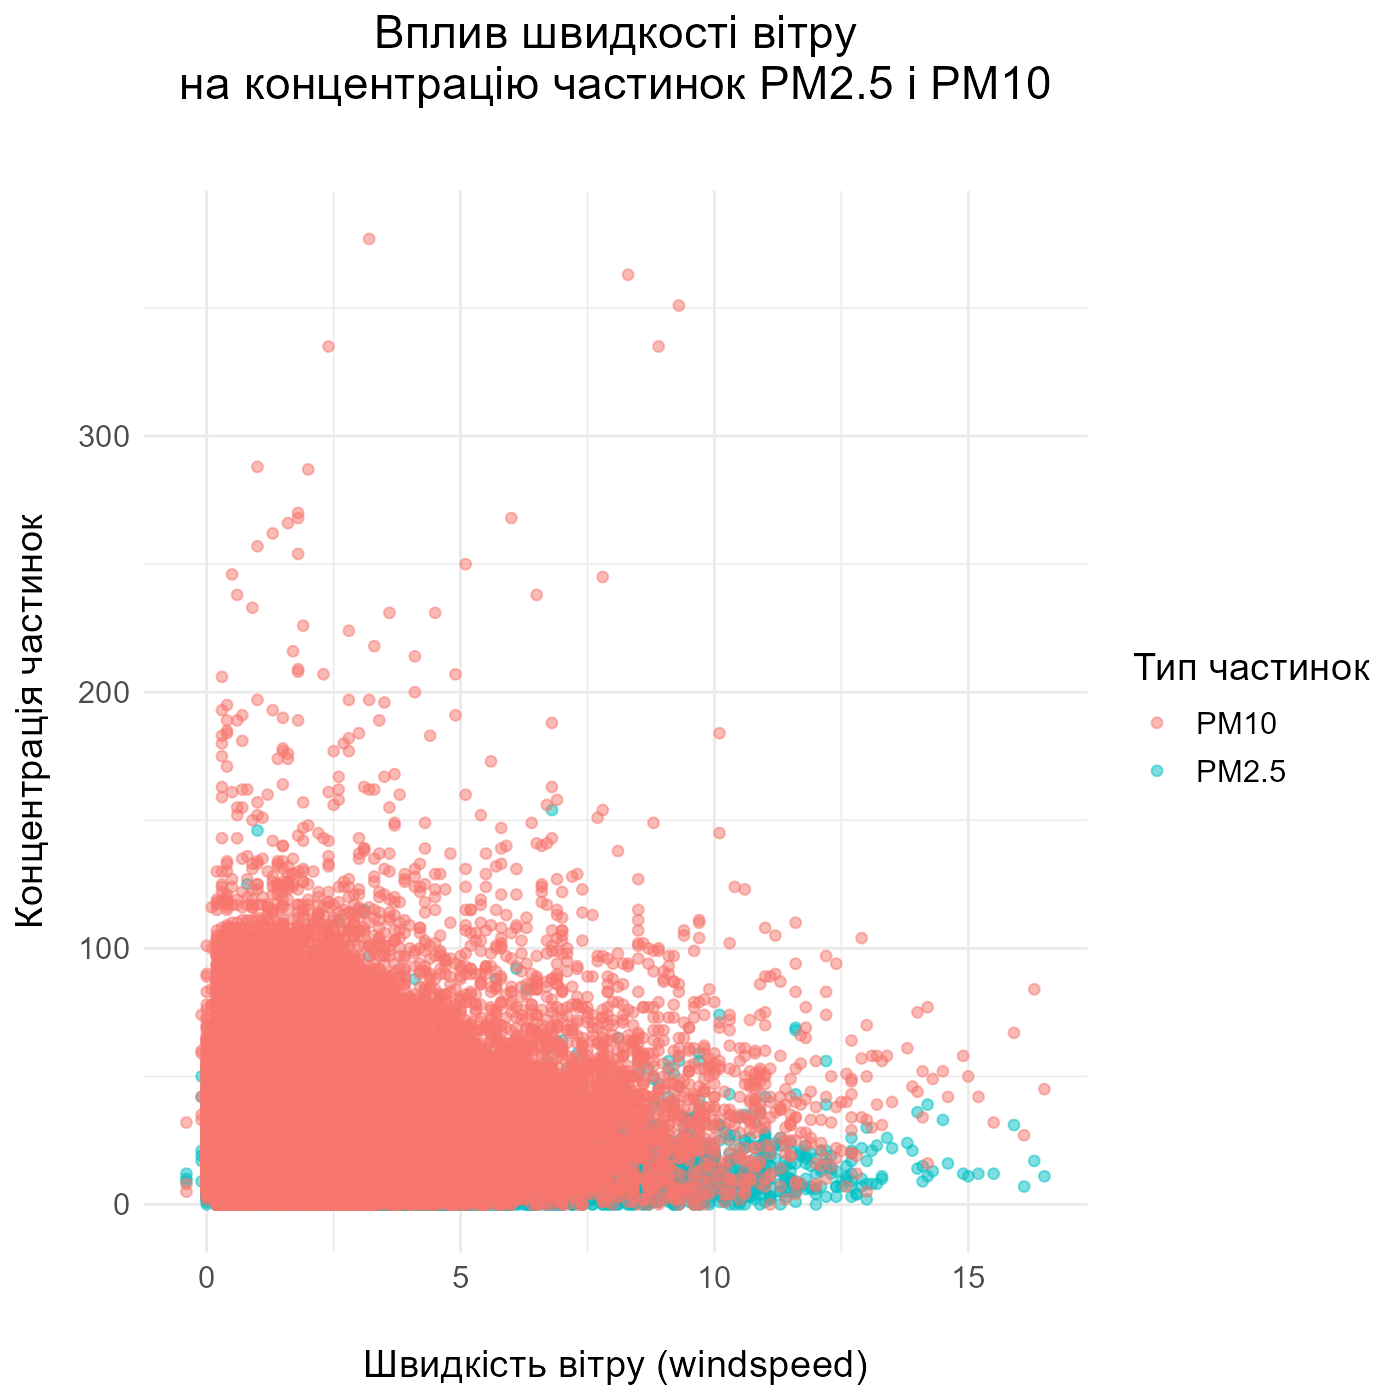
\includegraphics[width=\linewidth]{plots/question1/wind_speed_vs_pm.png}

  \pagebreak

  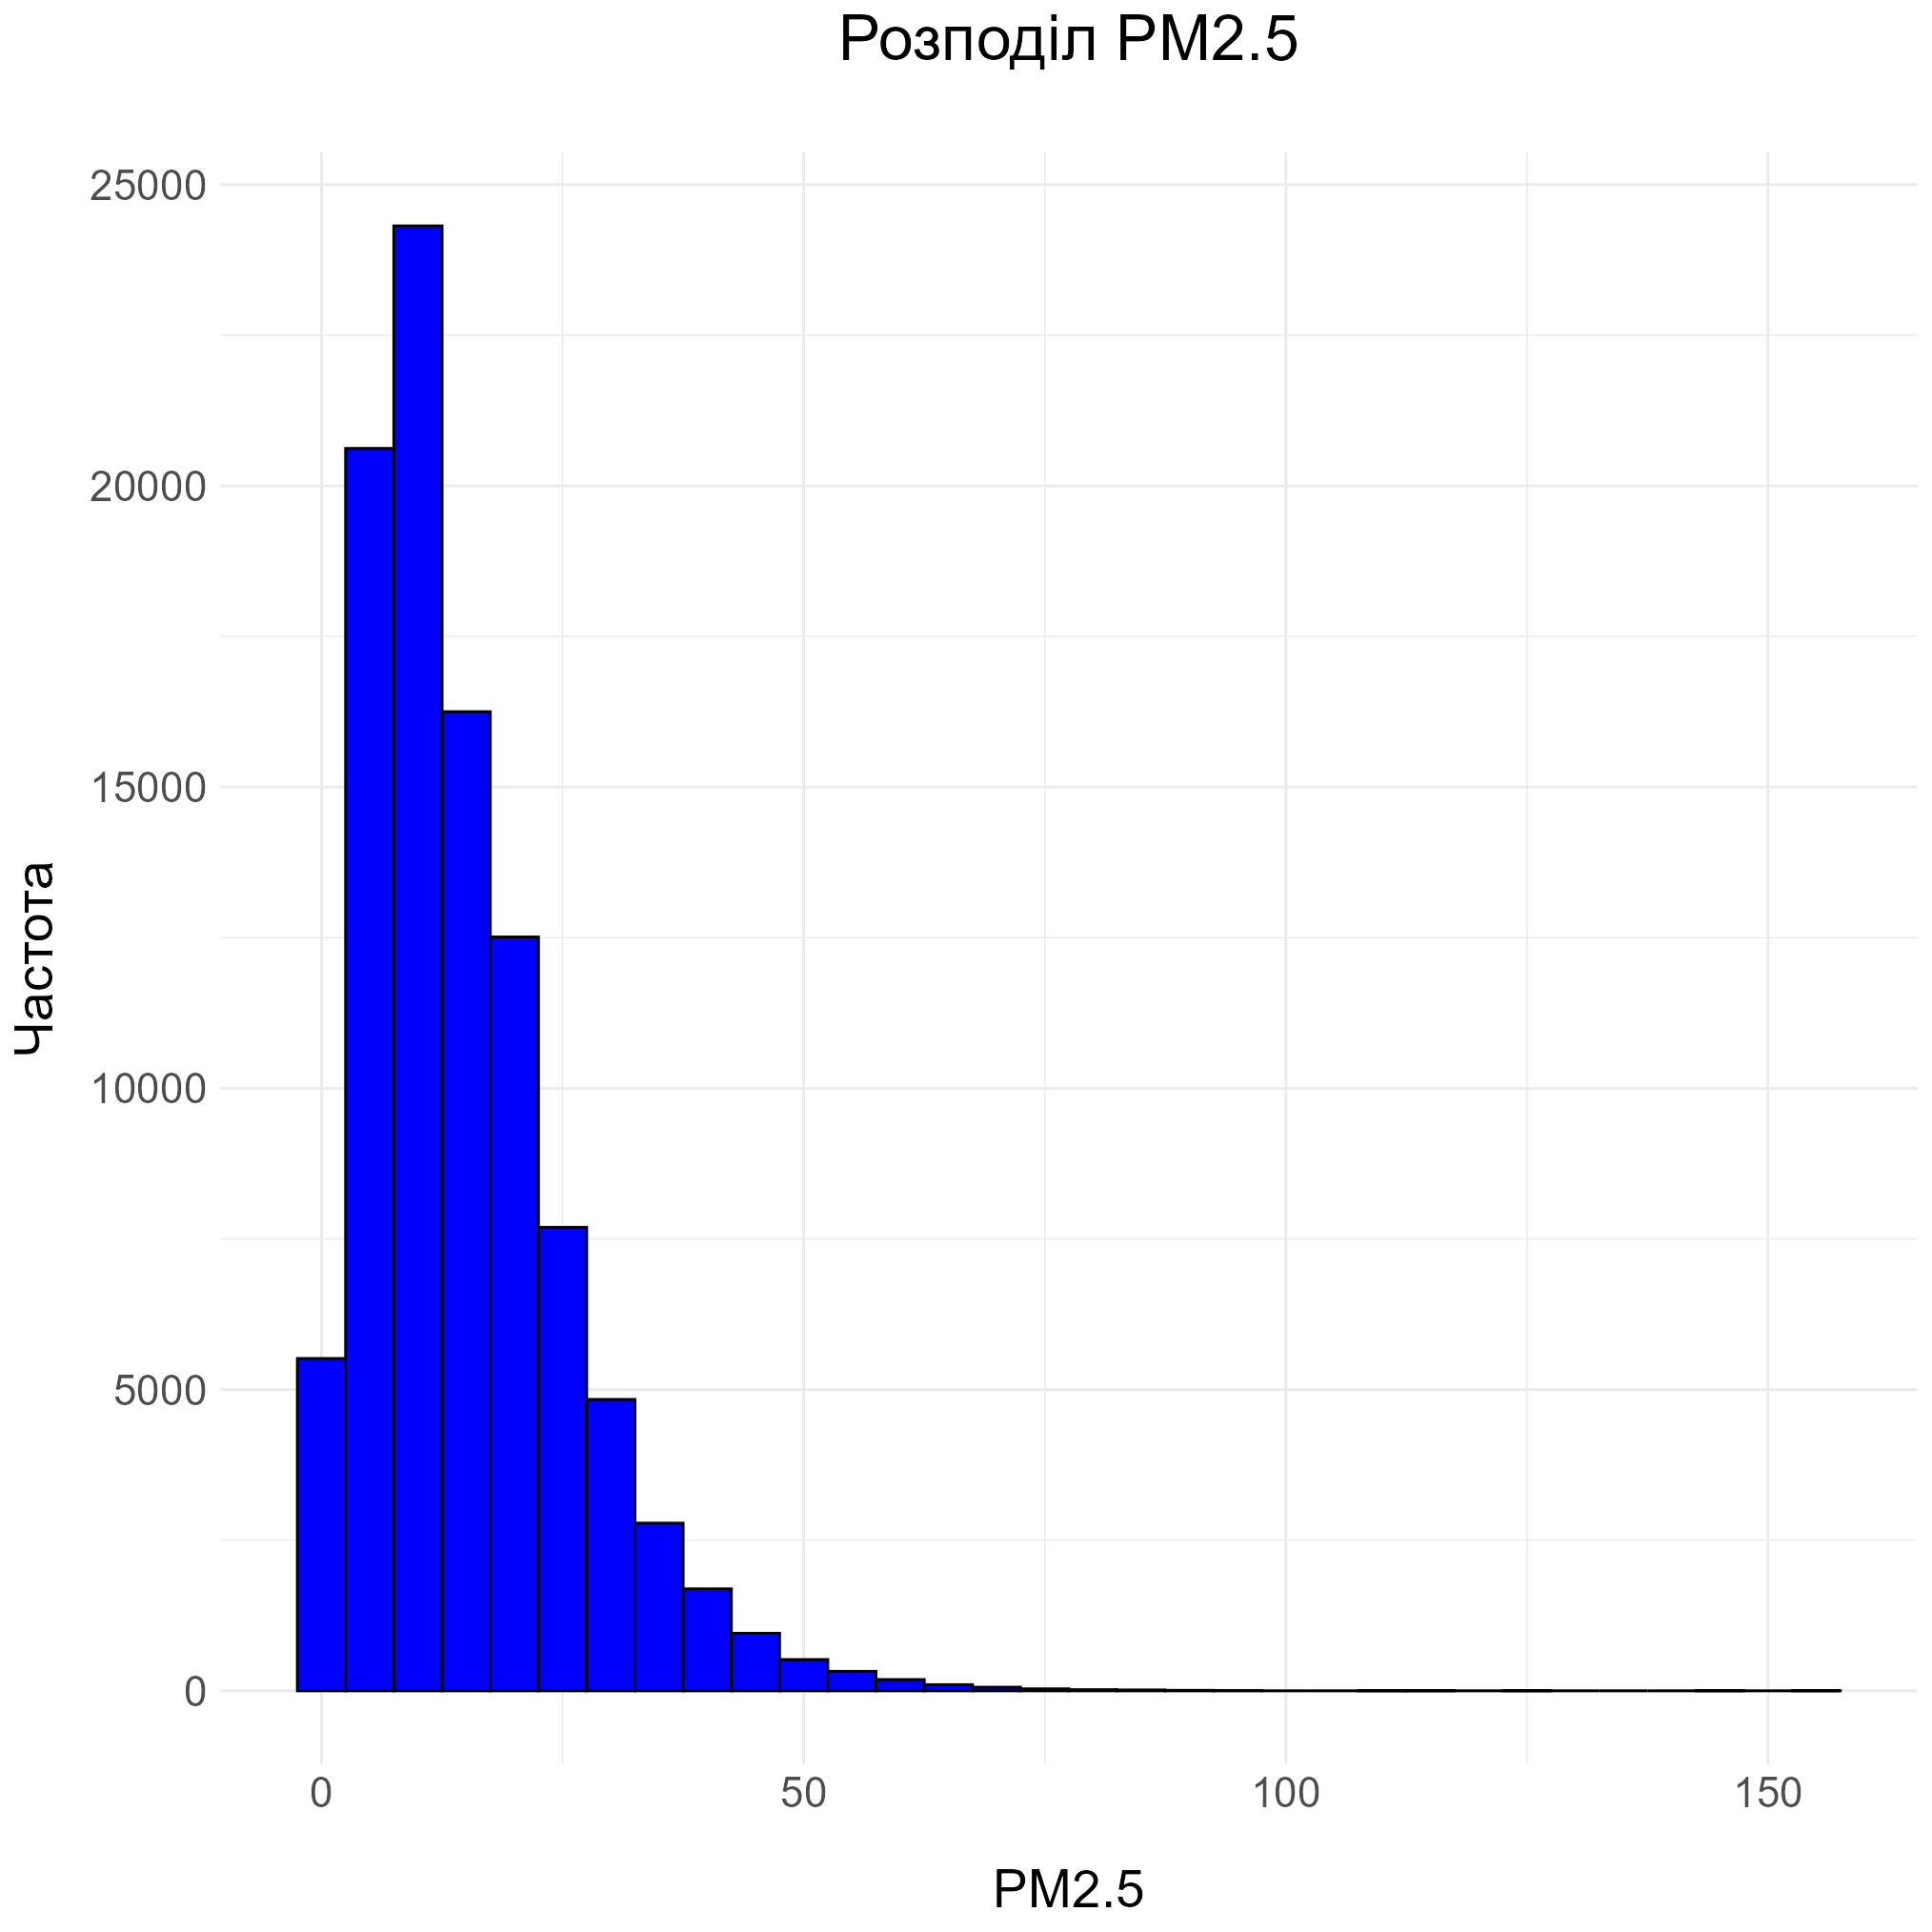
\includegraphics[width=\linewidth]{plots/question1/pm2_5_gist.png}

  \pagebreak

  Кореляційна матриця:

  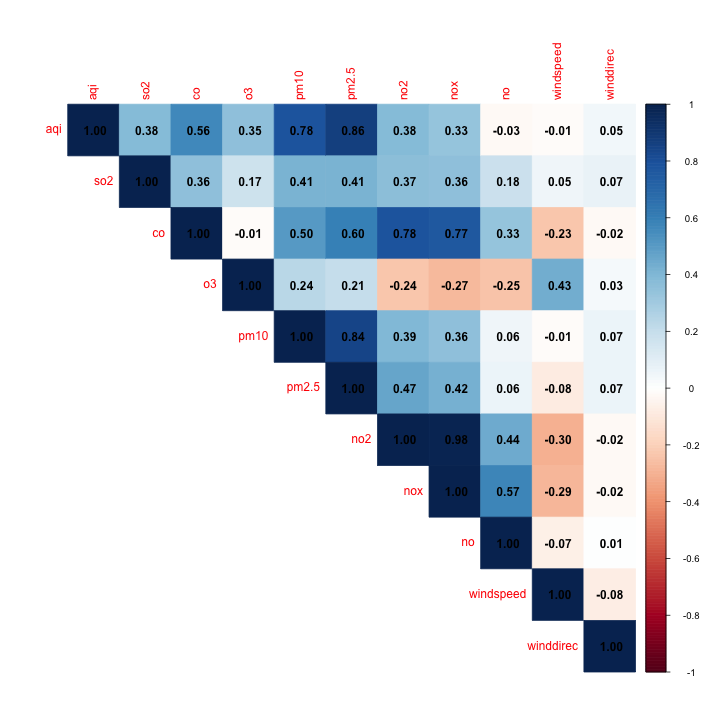
\includegraphics[width=\linewidth]{plots/question1/corr_matrix_plot.png}

  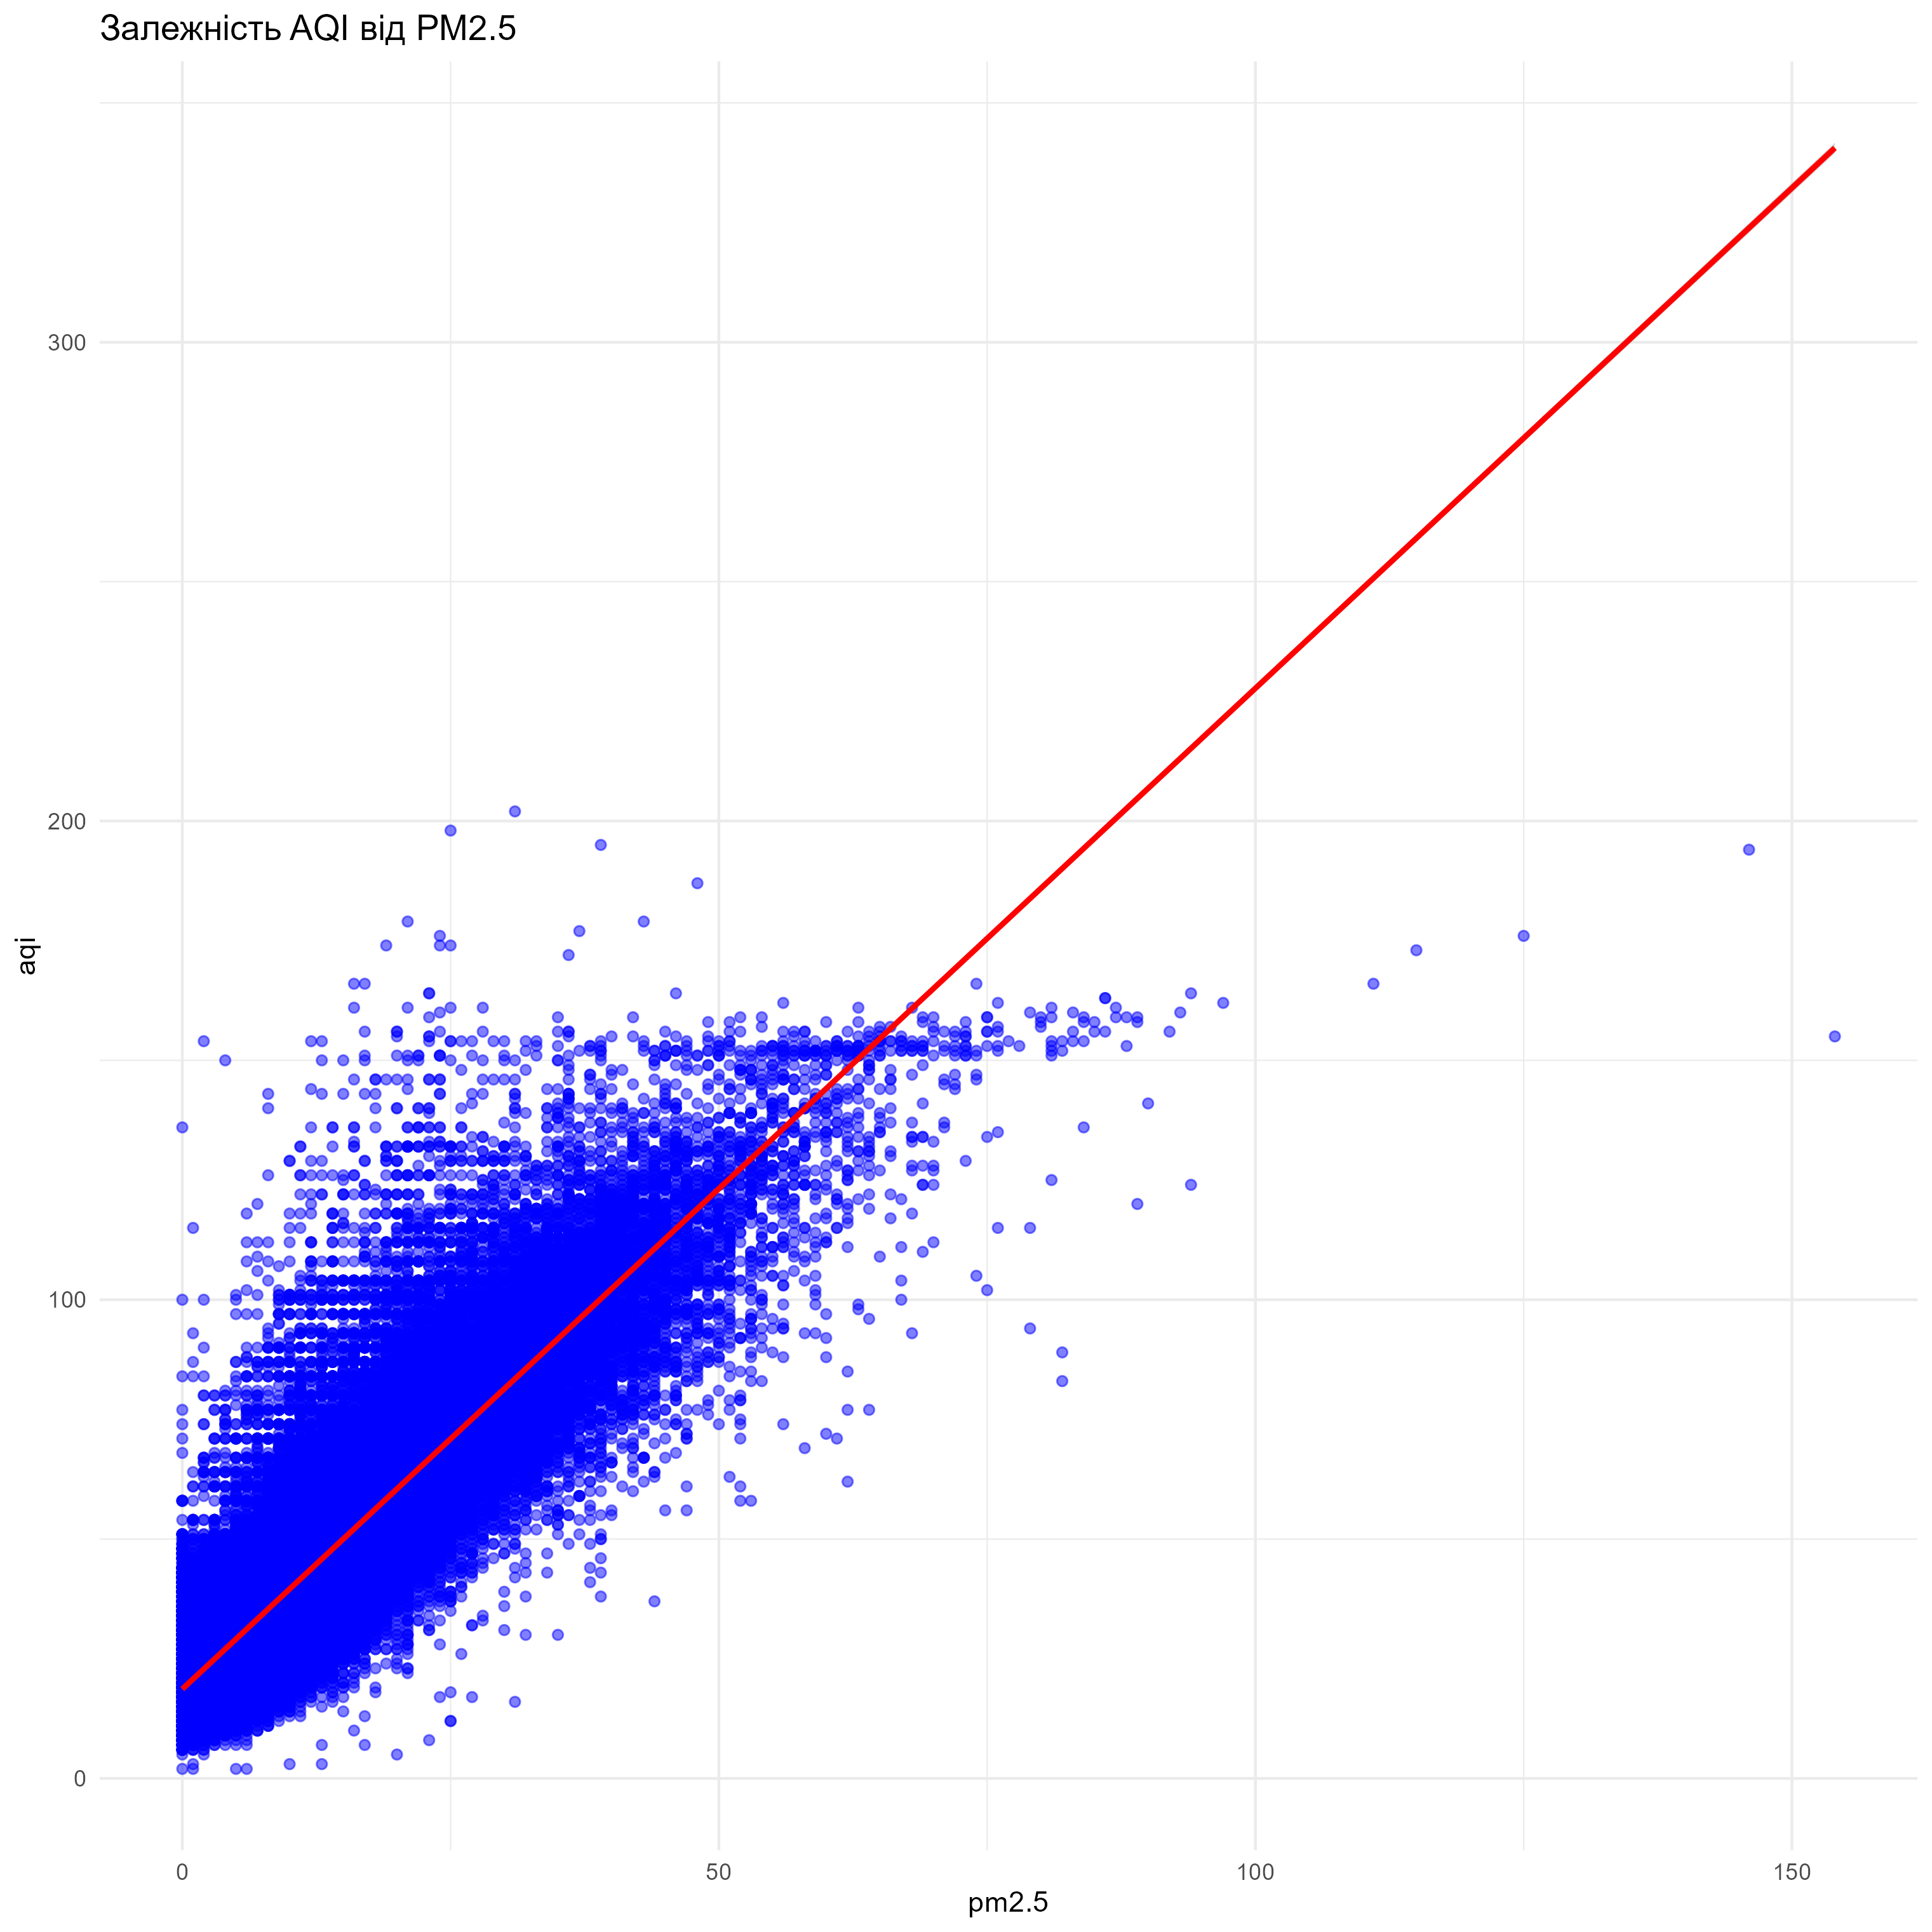
\includegraphics[width=\linewidth]{plots/question1/aqi_pm2_5_diagram.png}

  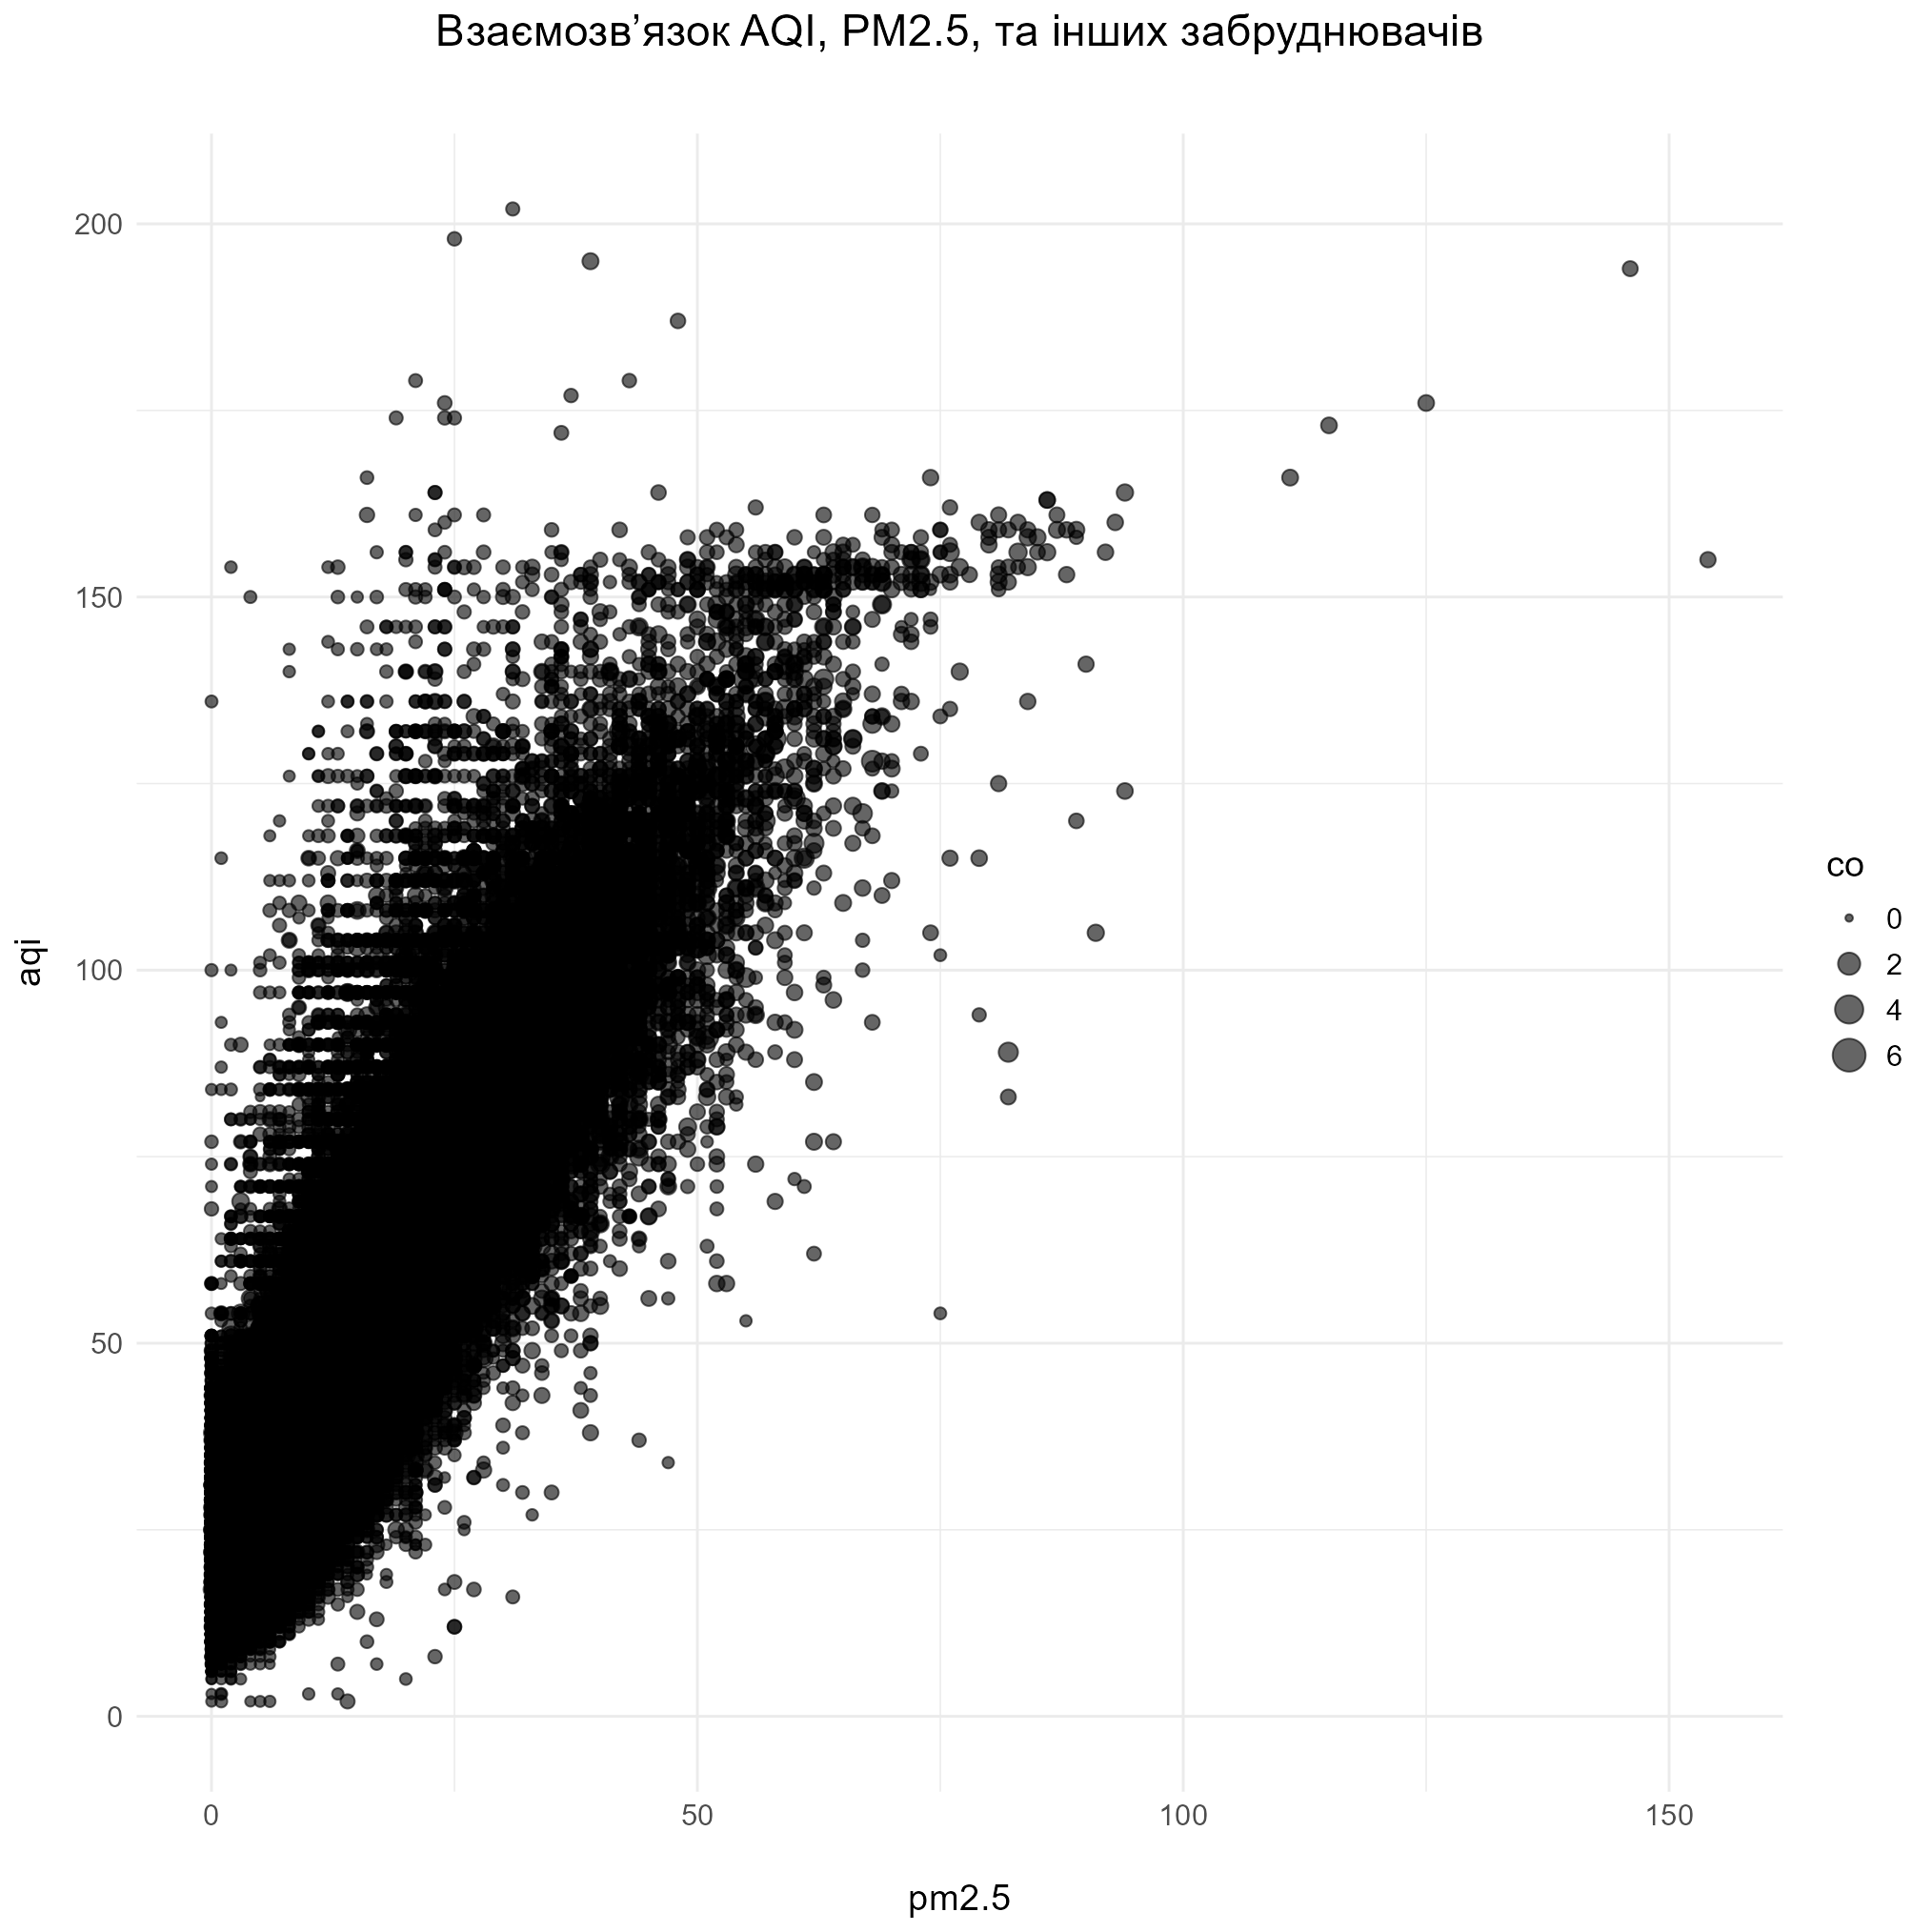
\includegraphics[width=\linewidth]{plots/question1/aqi_pm_polutants.png}

  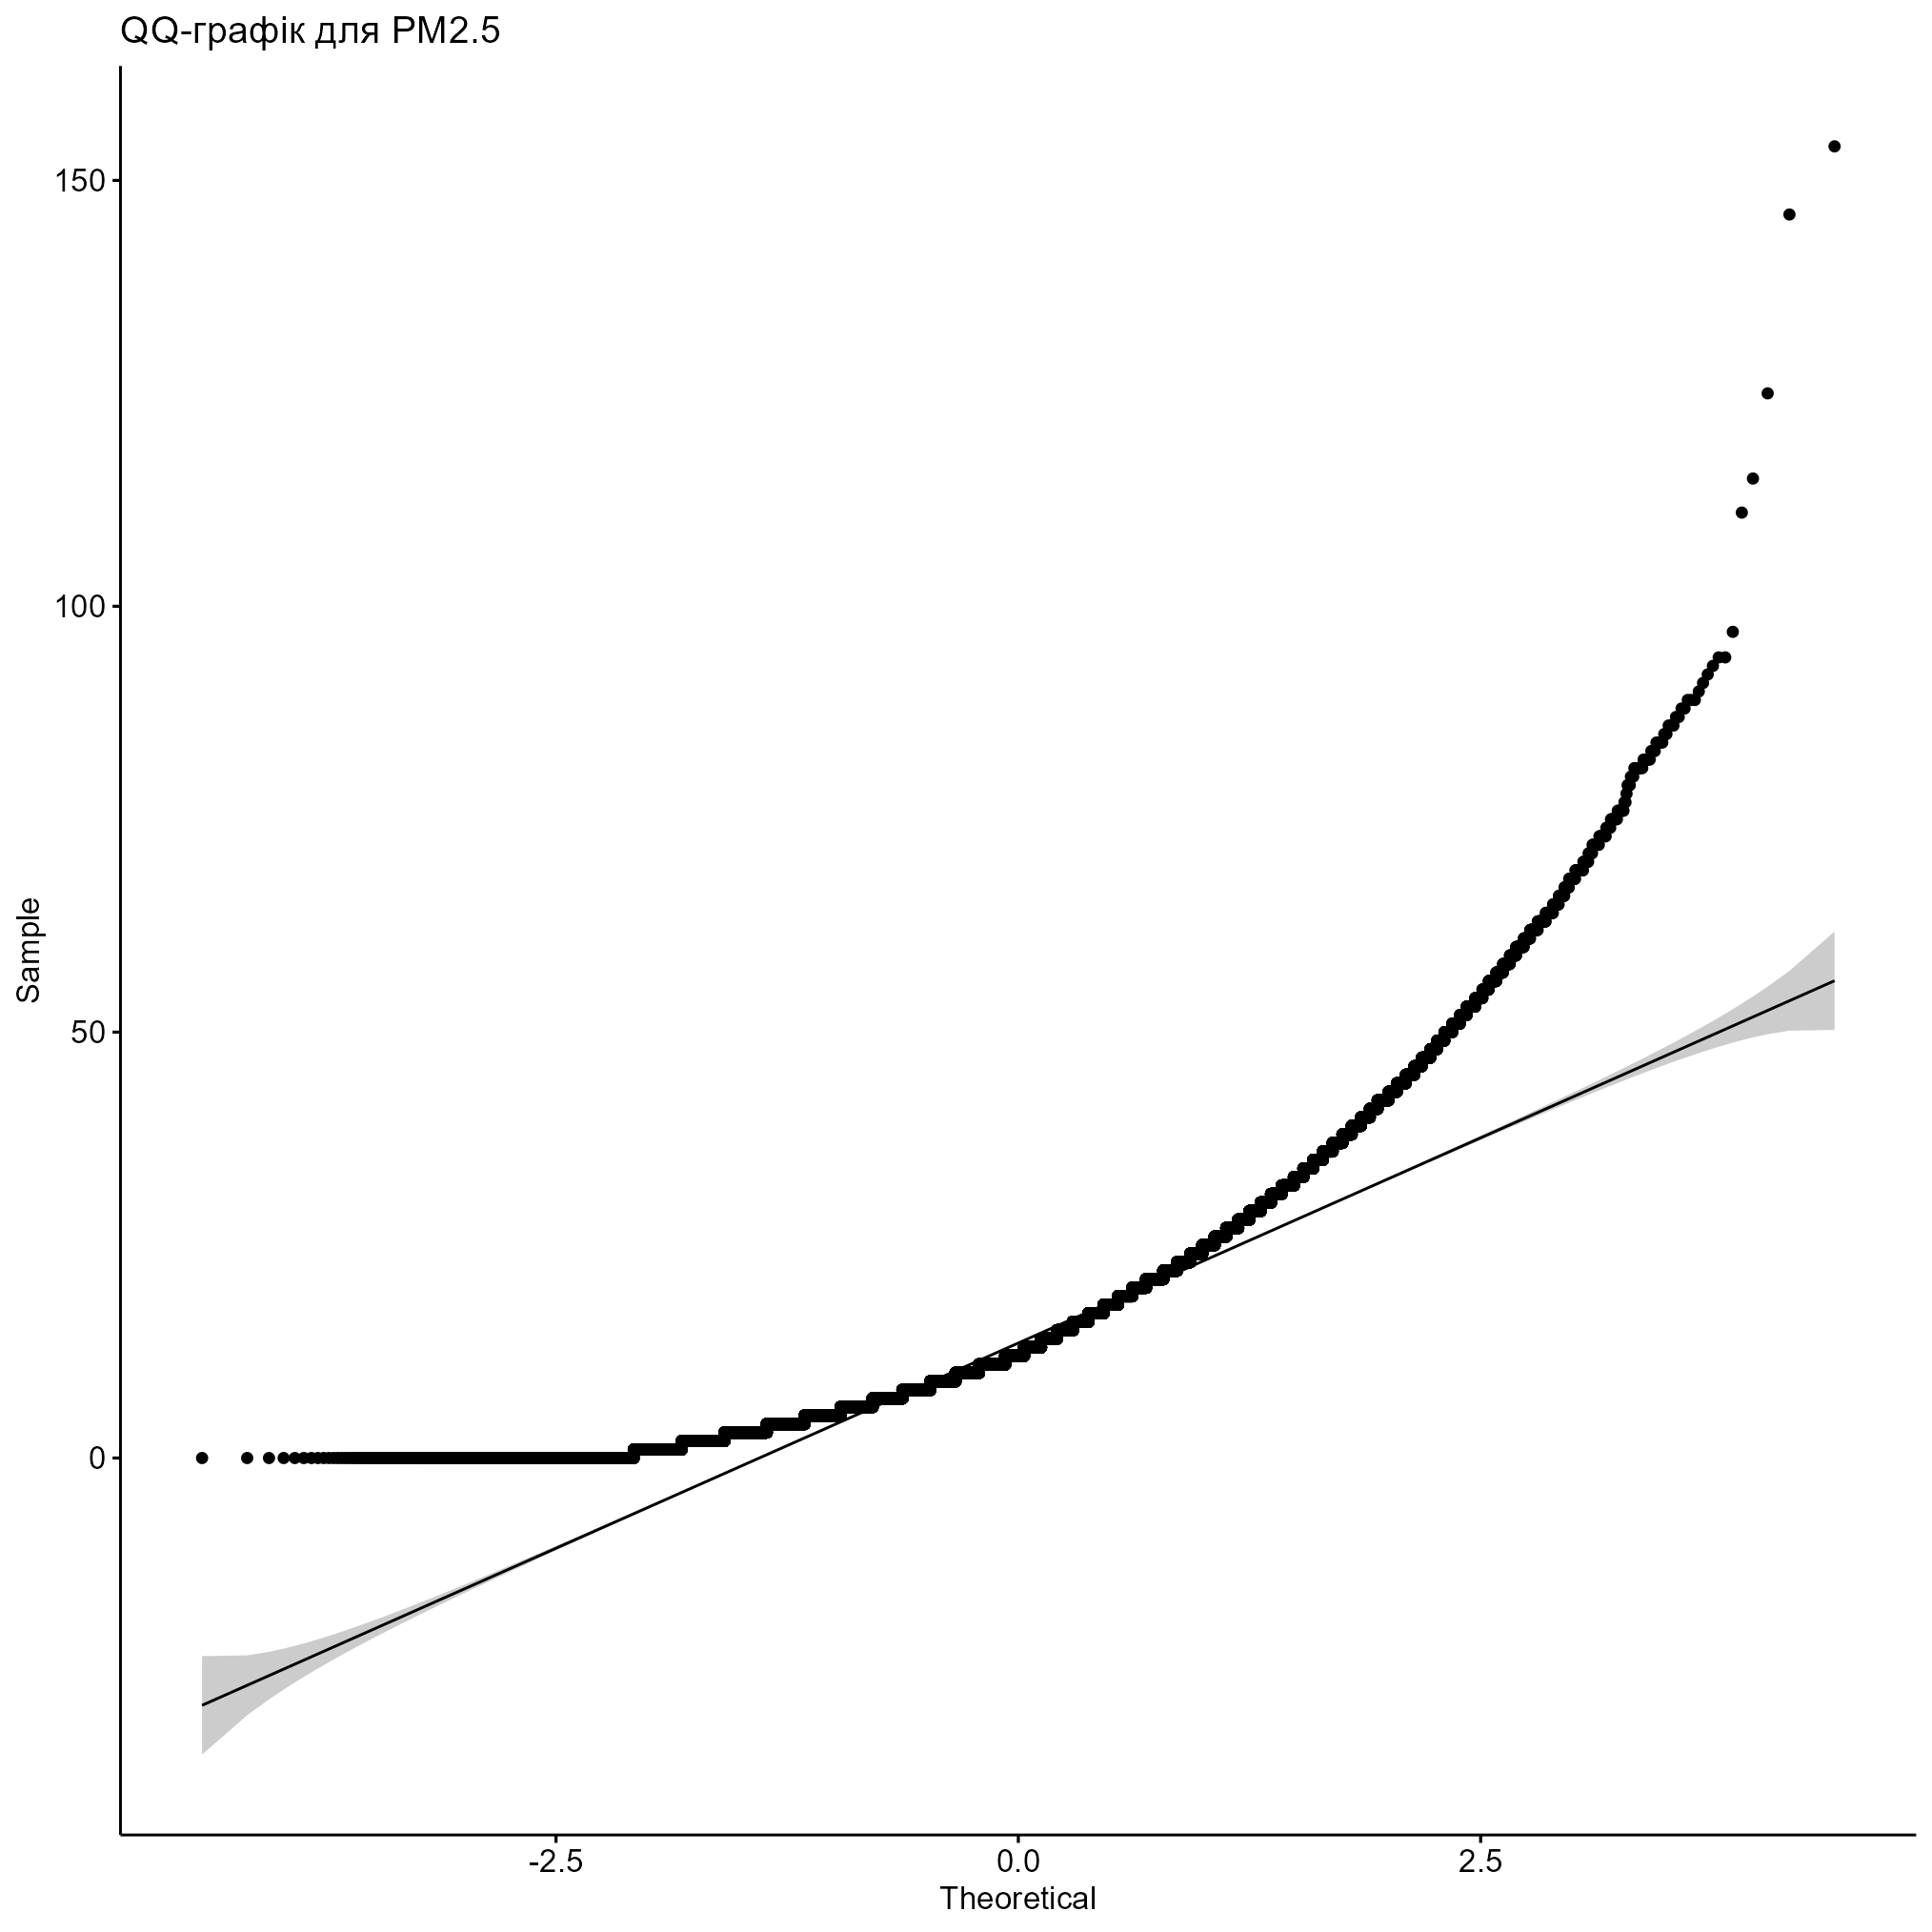
\includegraphics[width=\linewidth]{plots/question1/qq_pm2_5.png}

  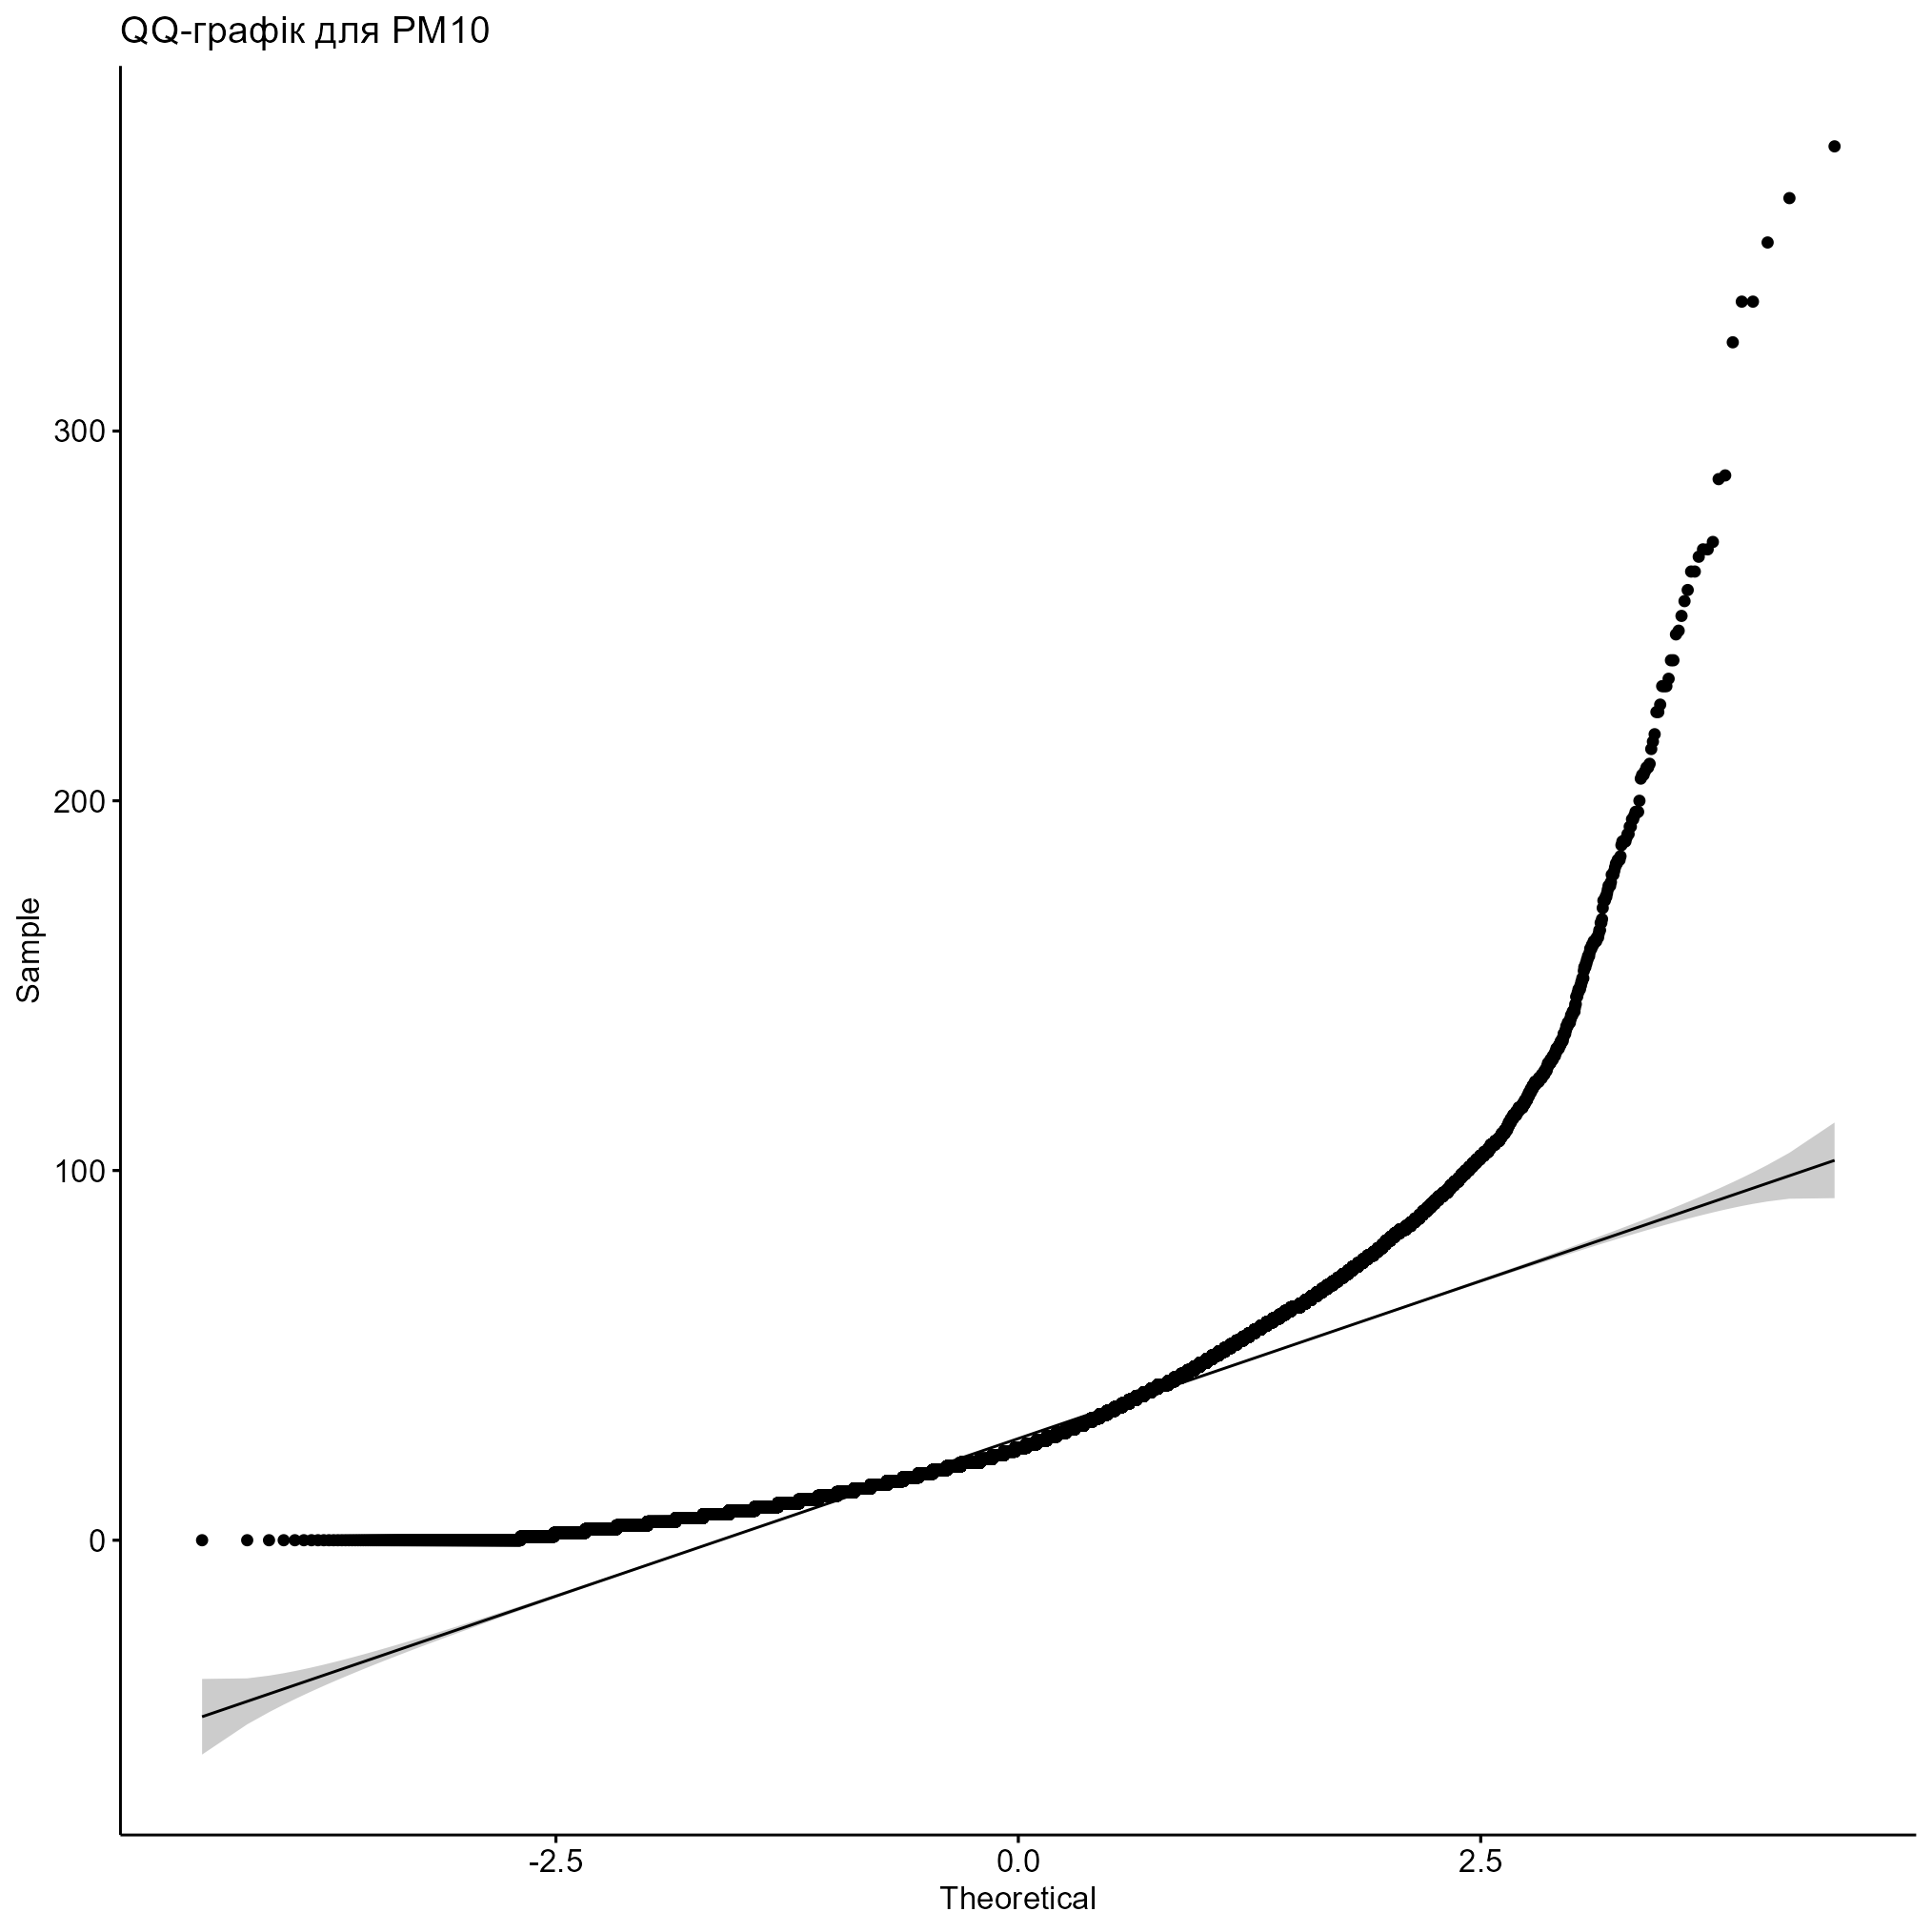
\includegraphics[width=\linewidth]{plots/question1/qq_pm10.png}

  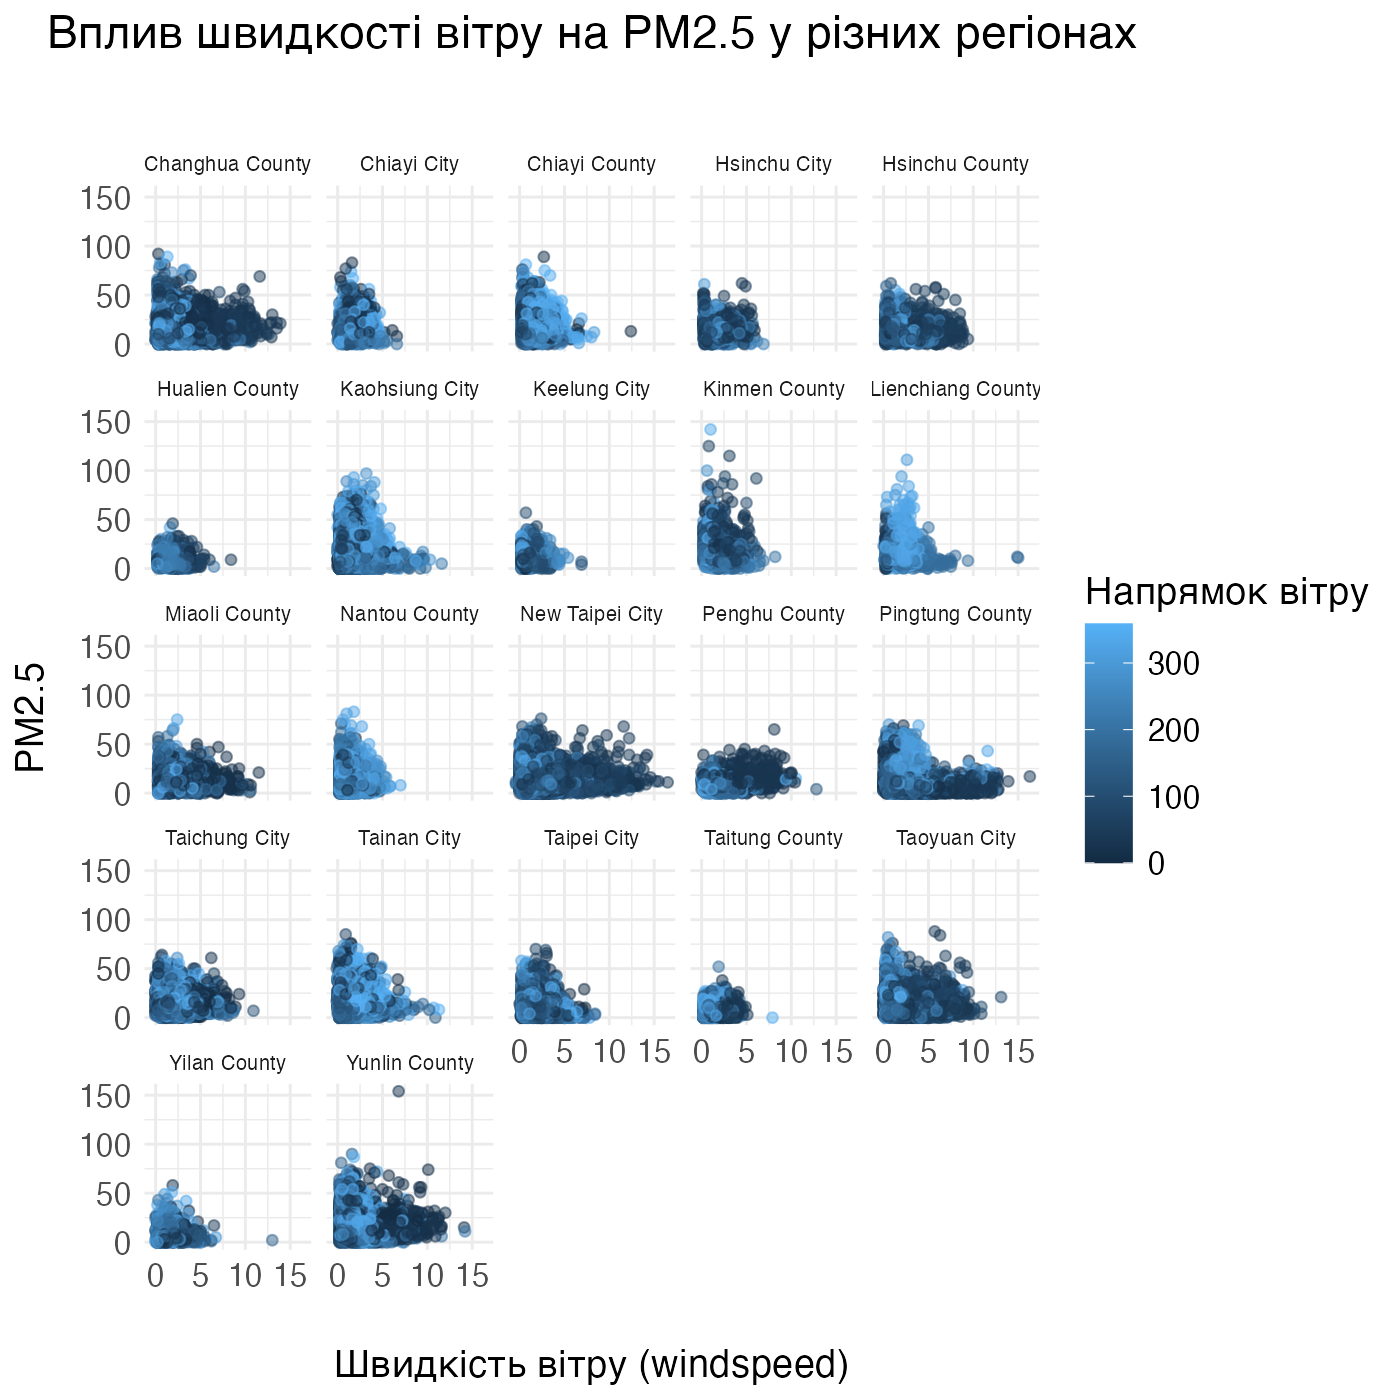
\includegraphics[width=\linewidth]{plots/question1/scatter_pm2_5_region.png}

  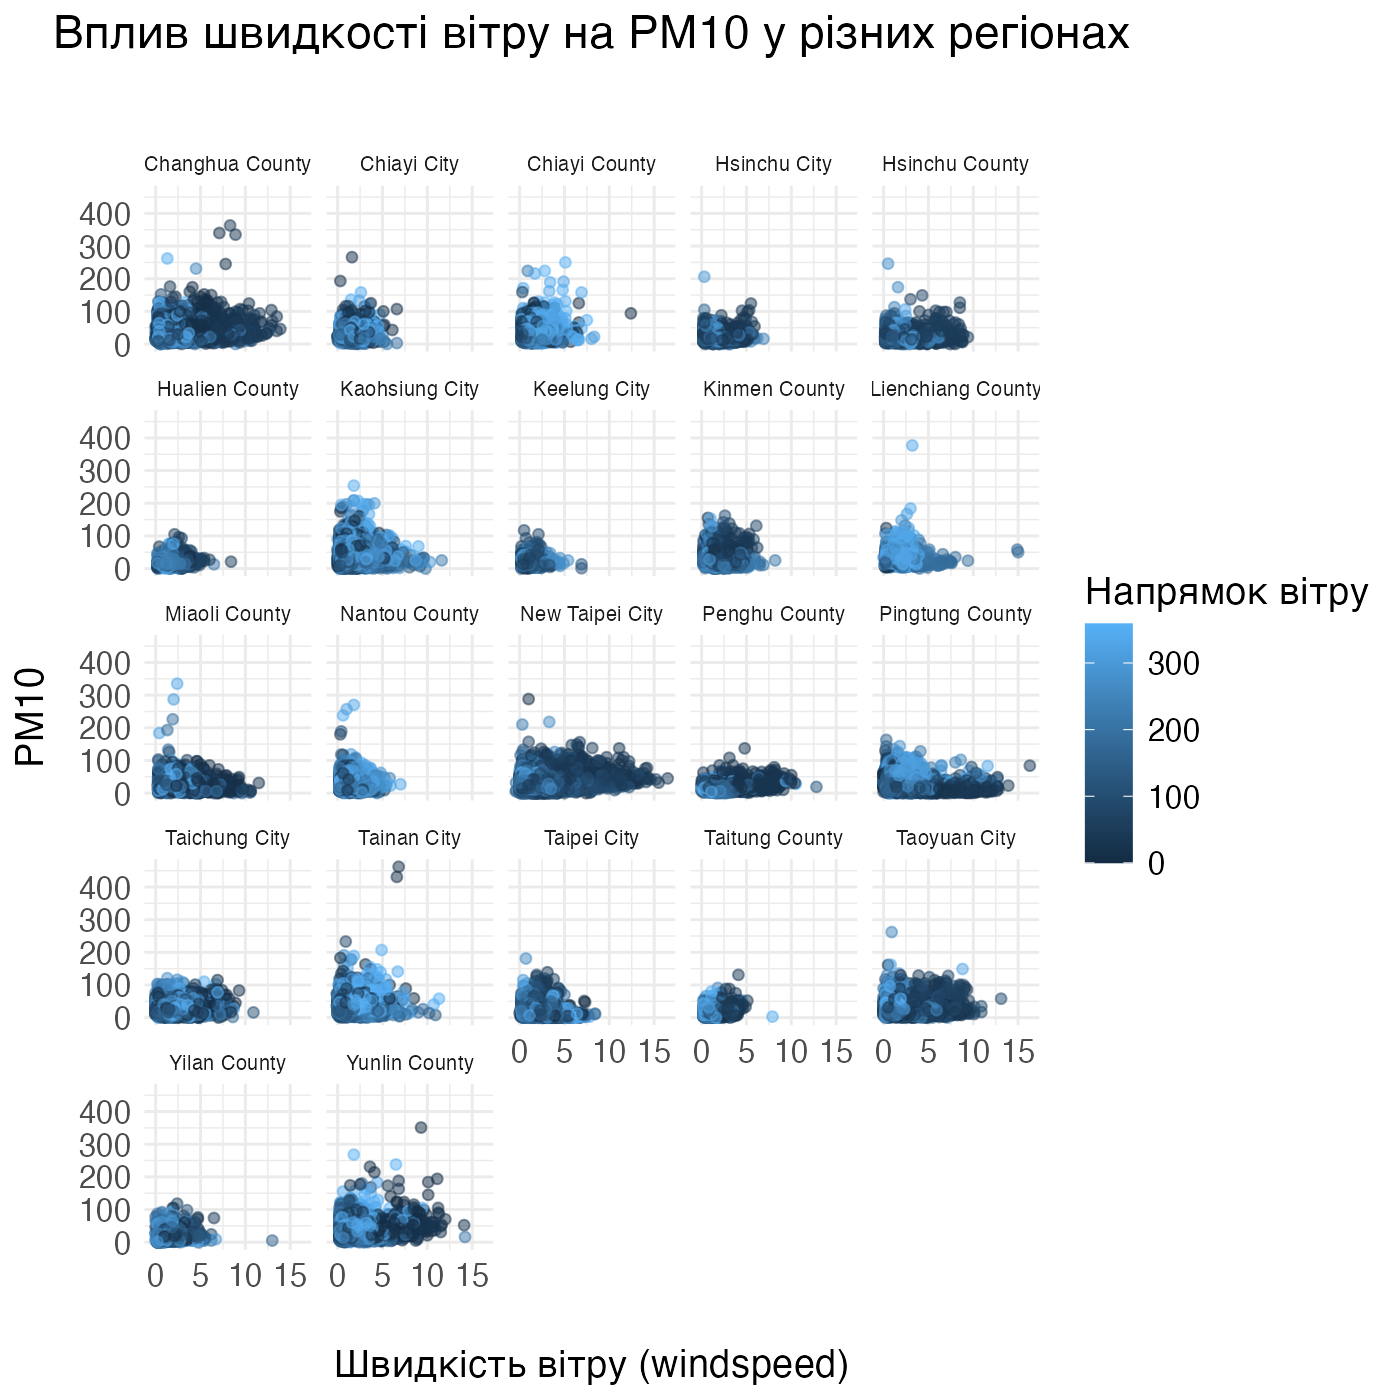
\includegraphics[width=\linewidth]{plots/question1/scatter_pm10_region.png}

  \pagebreak

  \item Як зміни в концентрації ($O_3$) та $SO_2$ впливають на загальний рівень забруднення повітря (AQI)?

  \quad \textit{Був використаний trimmed набір даних}

  Для початку дамо відповідь на питання:
  Чи є зв’язок між концентраціями різних забруднювачів? (кореляційна матриця)

  Аналіз викидів та розподілу всіх показників забруднення:

  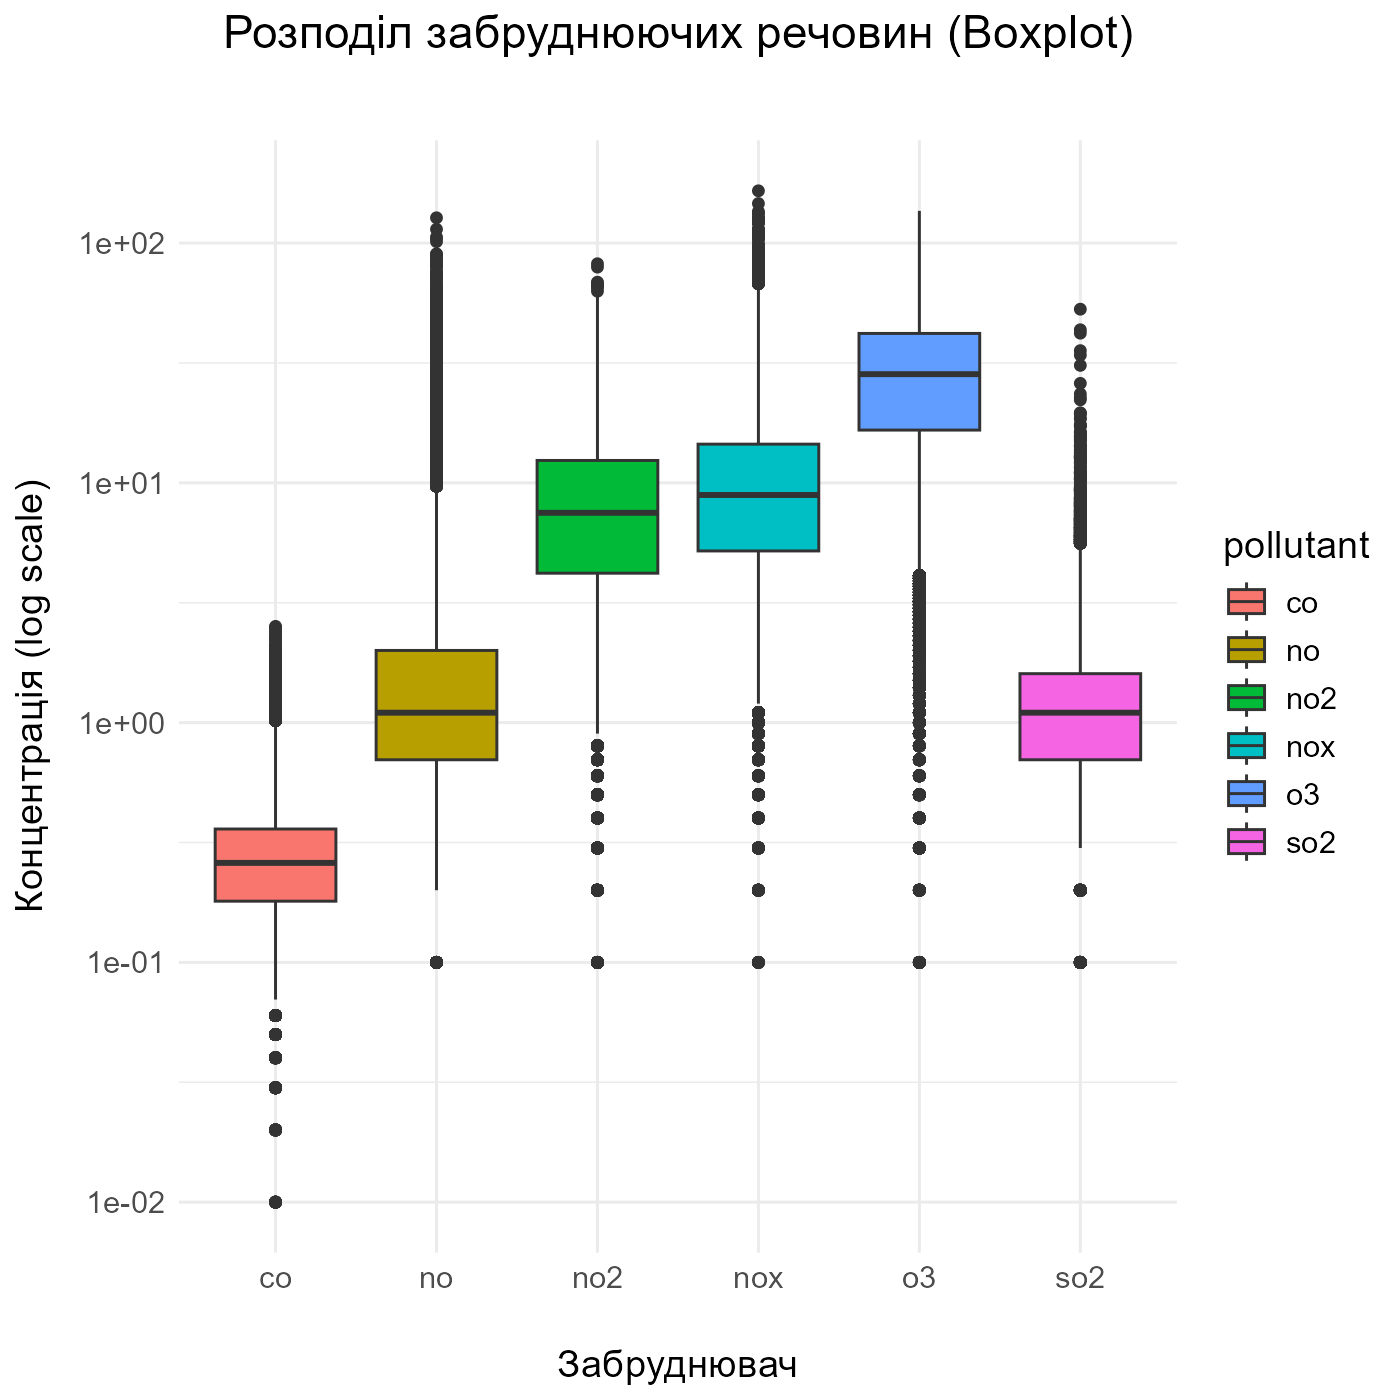
\includegraphics[width=\linewidth]{plots/question2/boxplot_pollutants.png}

  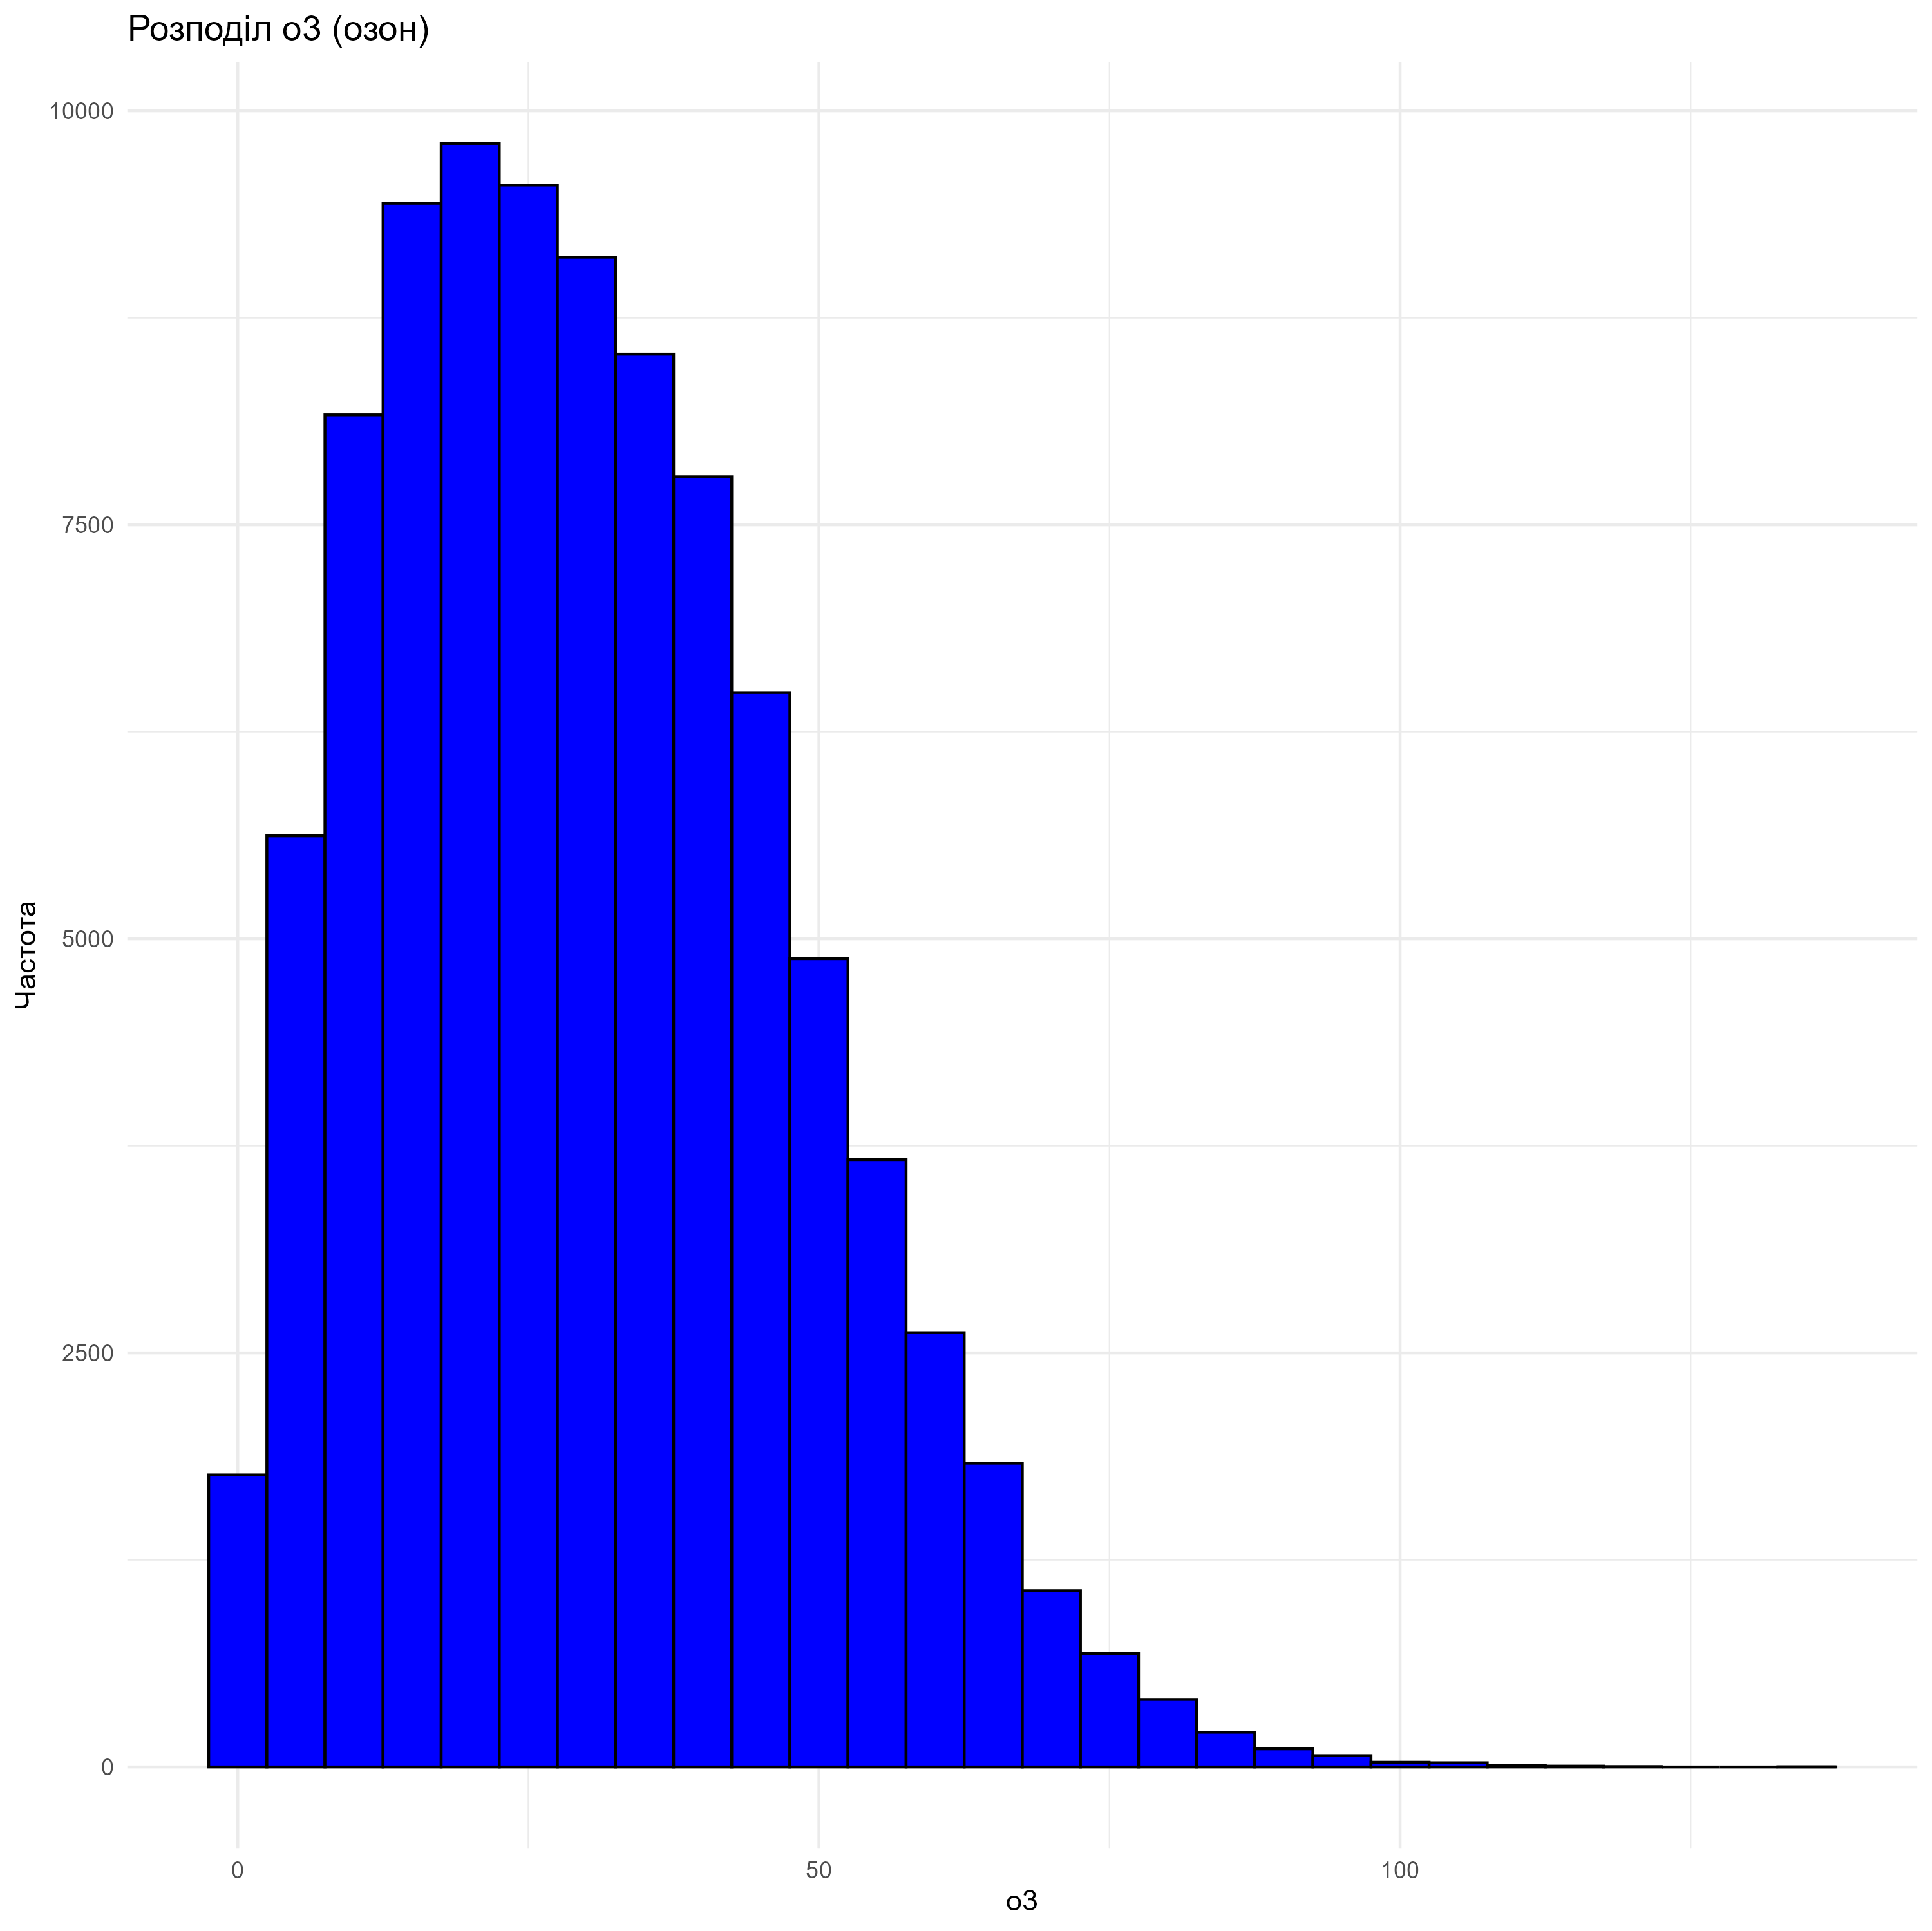
\includegraphics[width=\linewidth]{plots/question2/o3_plot.png}

  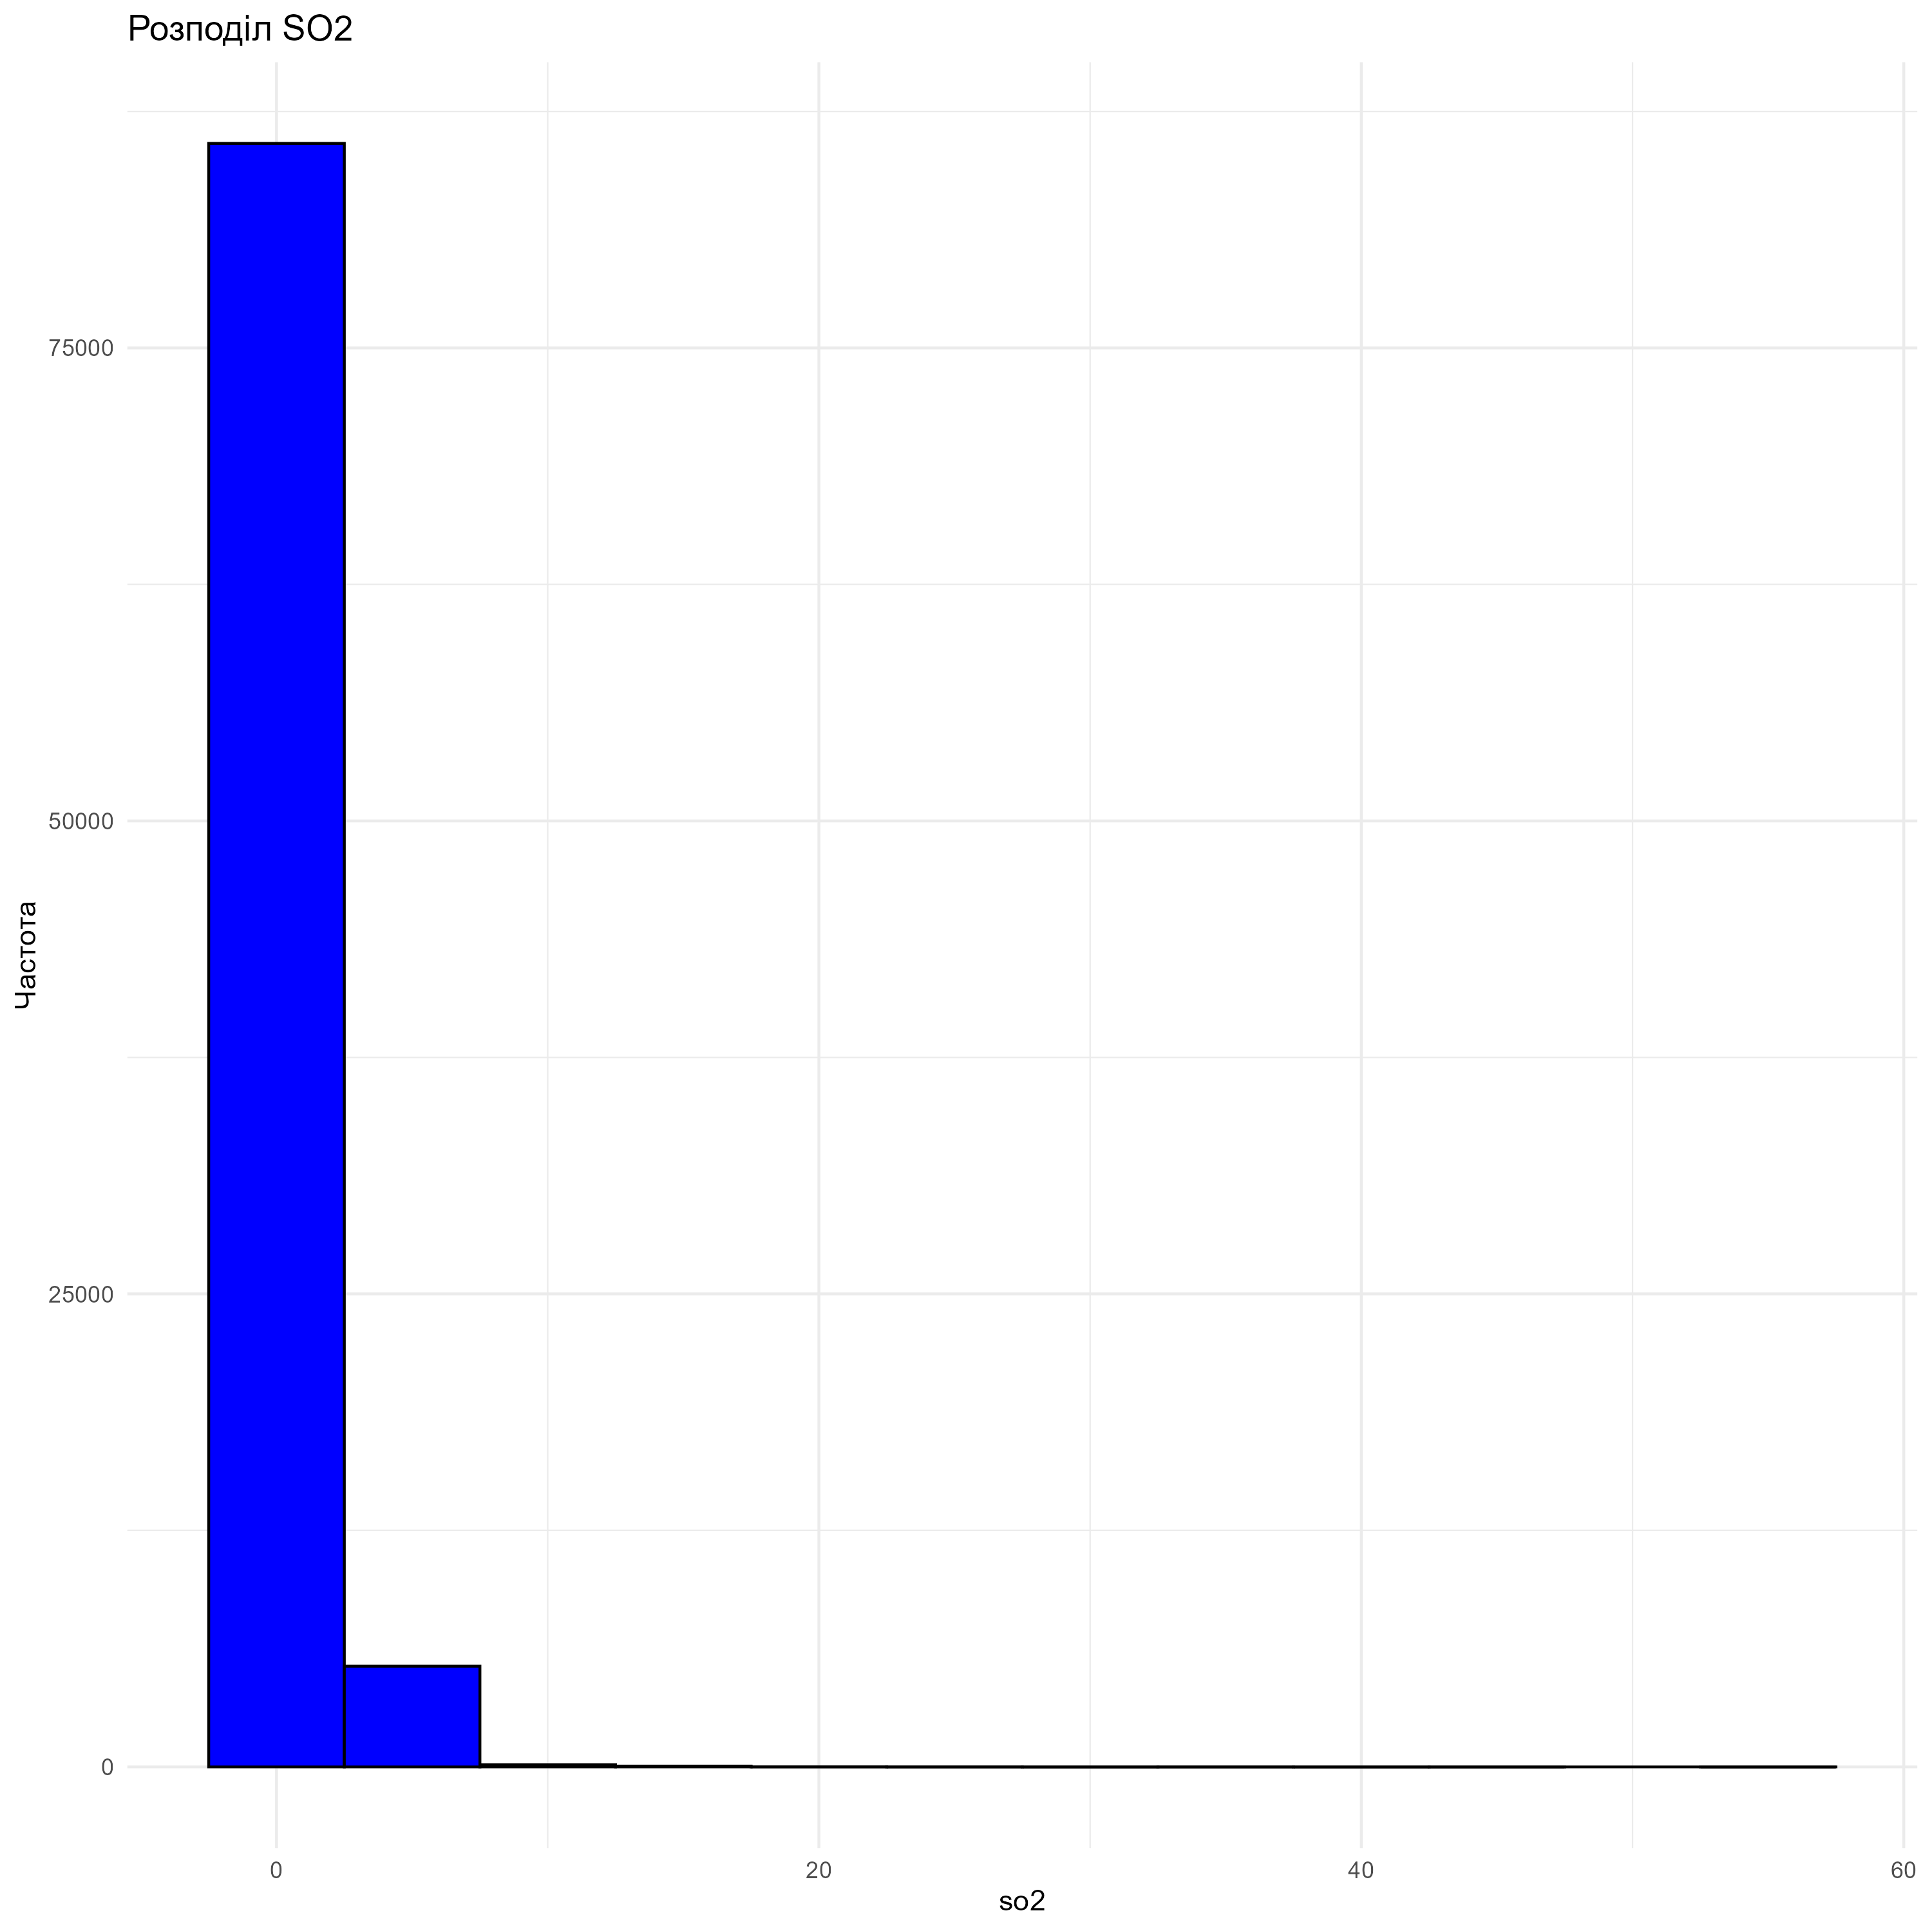
\includegraphics[width=\linewidth]{plots/question2/so2_plot.png}

  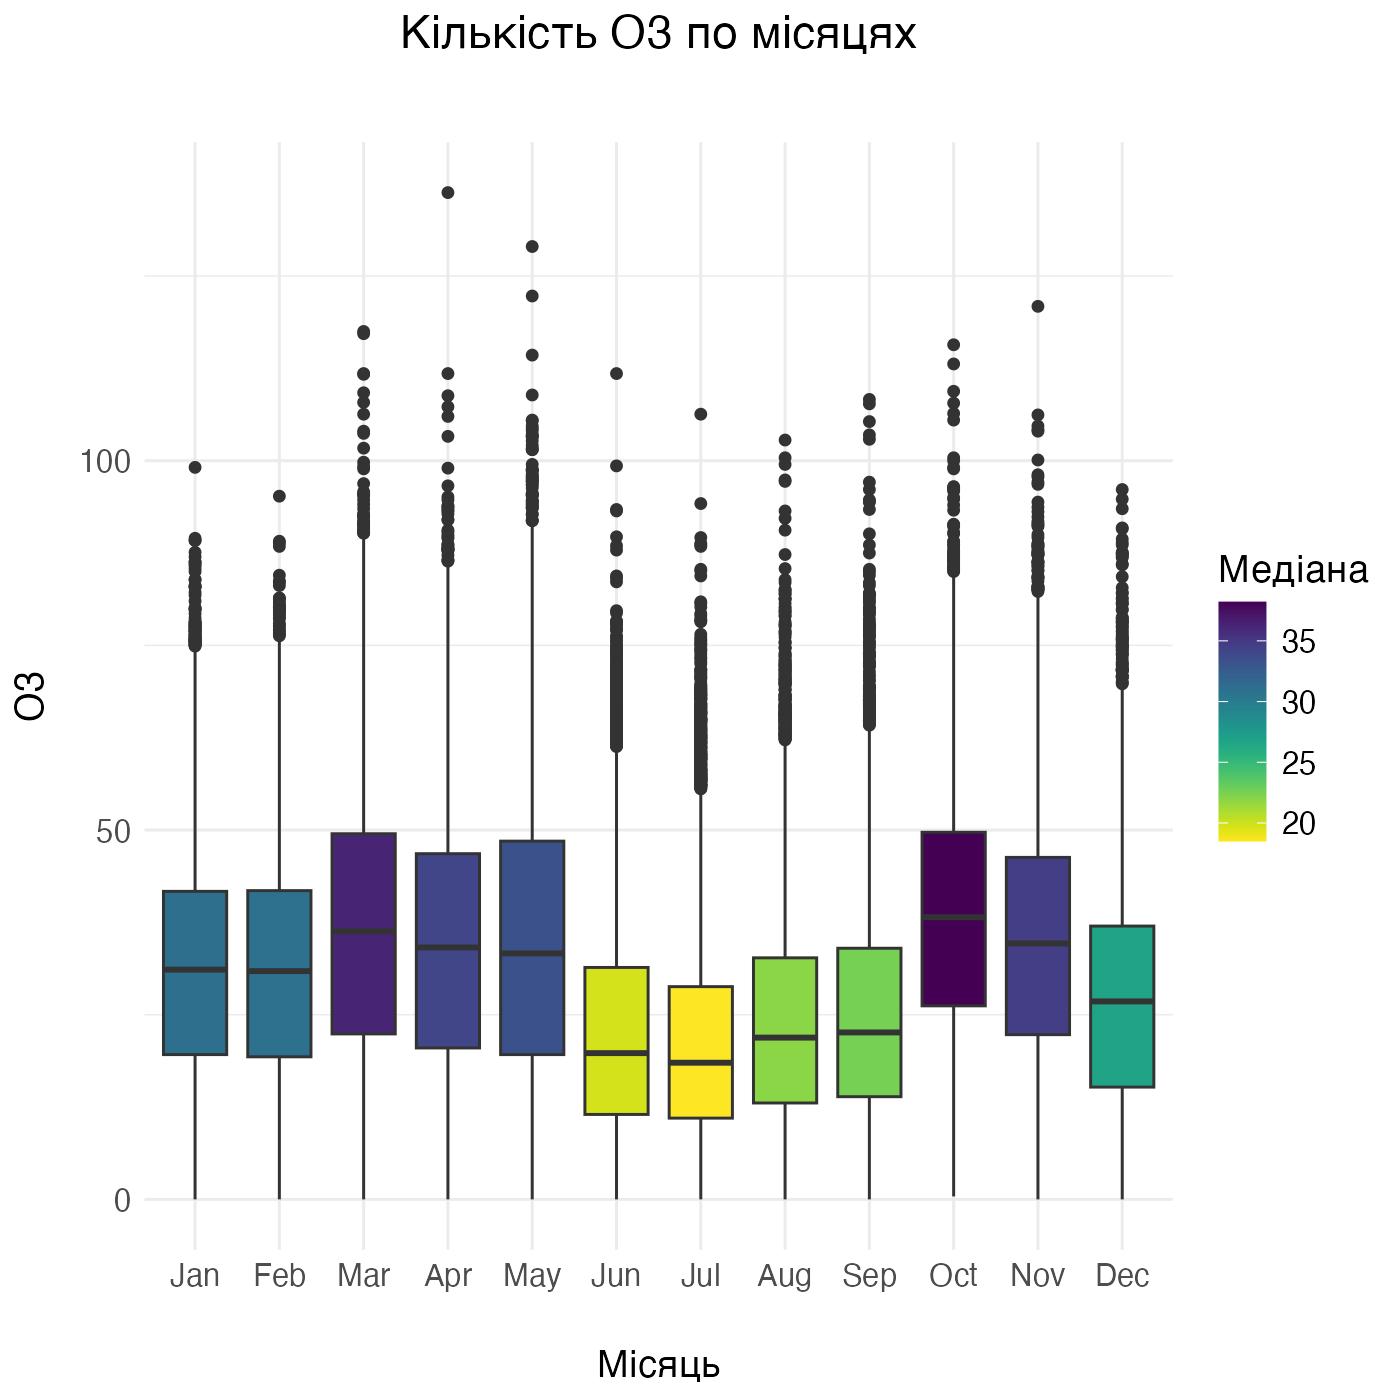
\includegraphics[width=\linewidth]{plots/question2/seasonal_o3.png}

  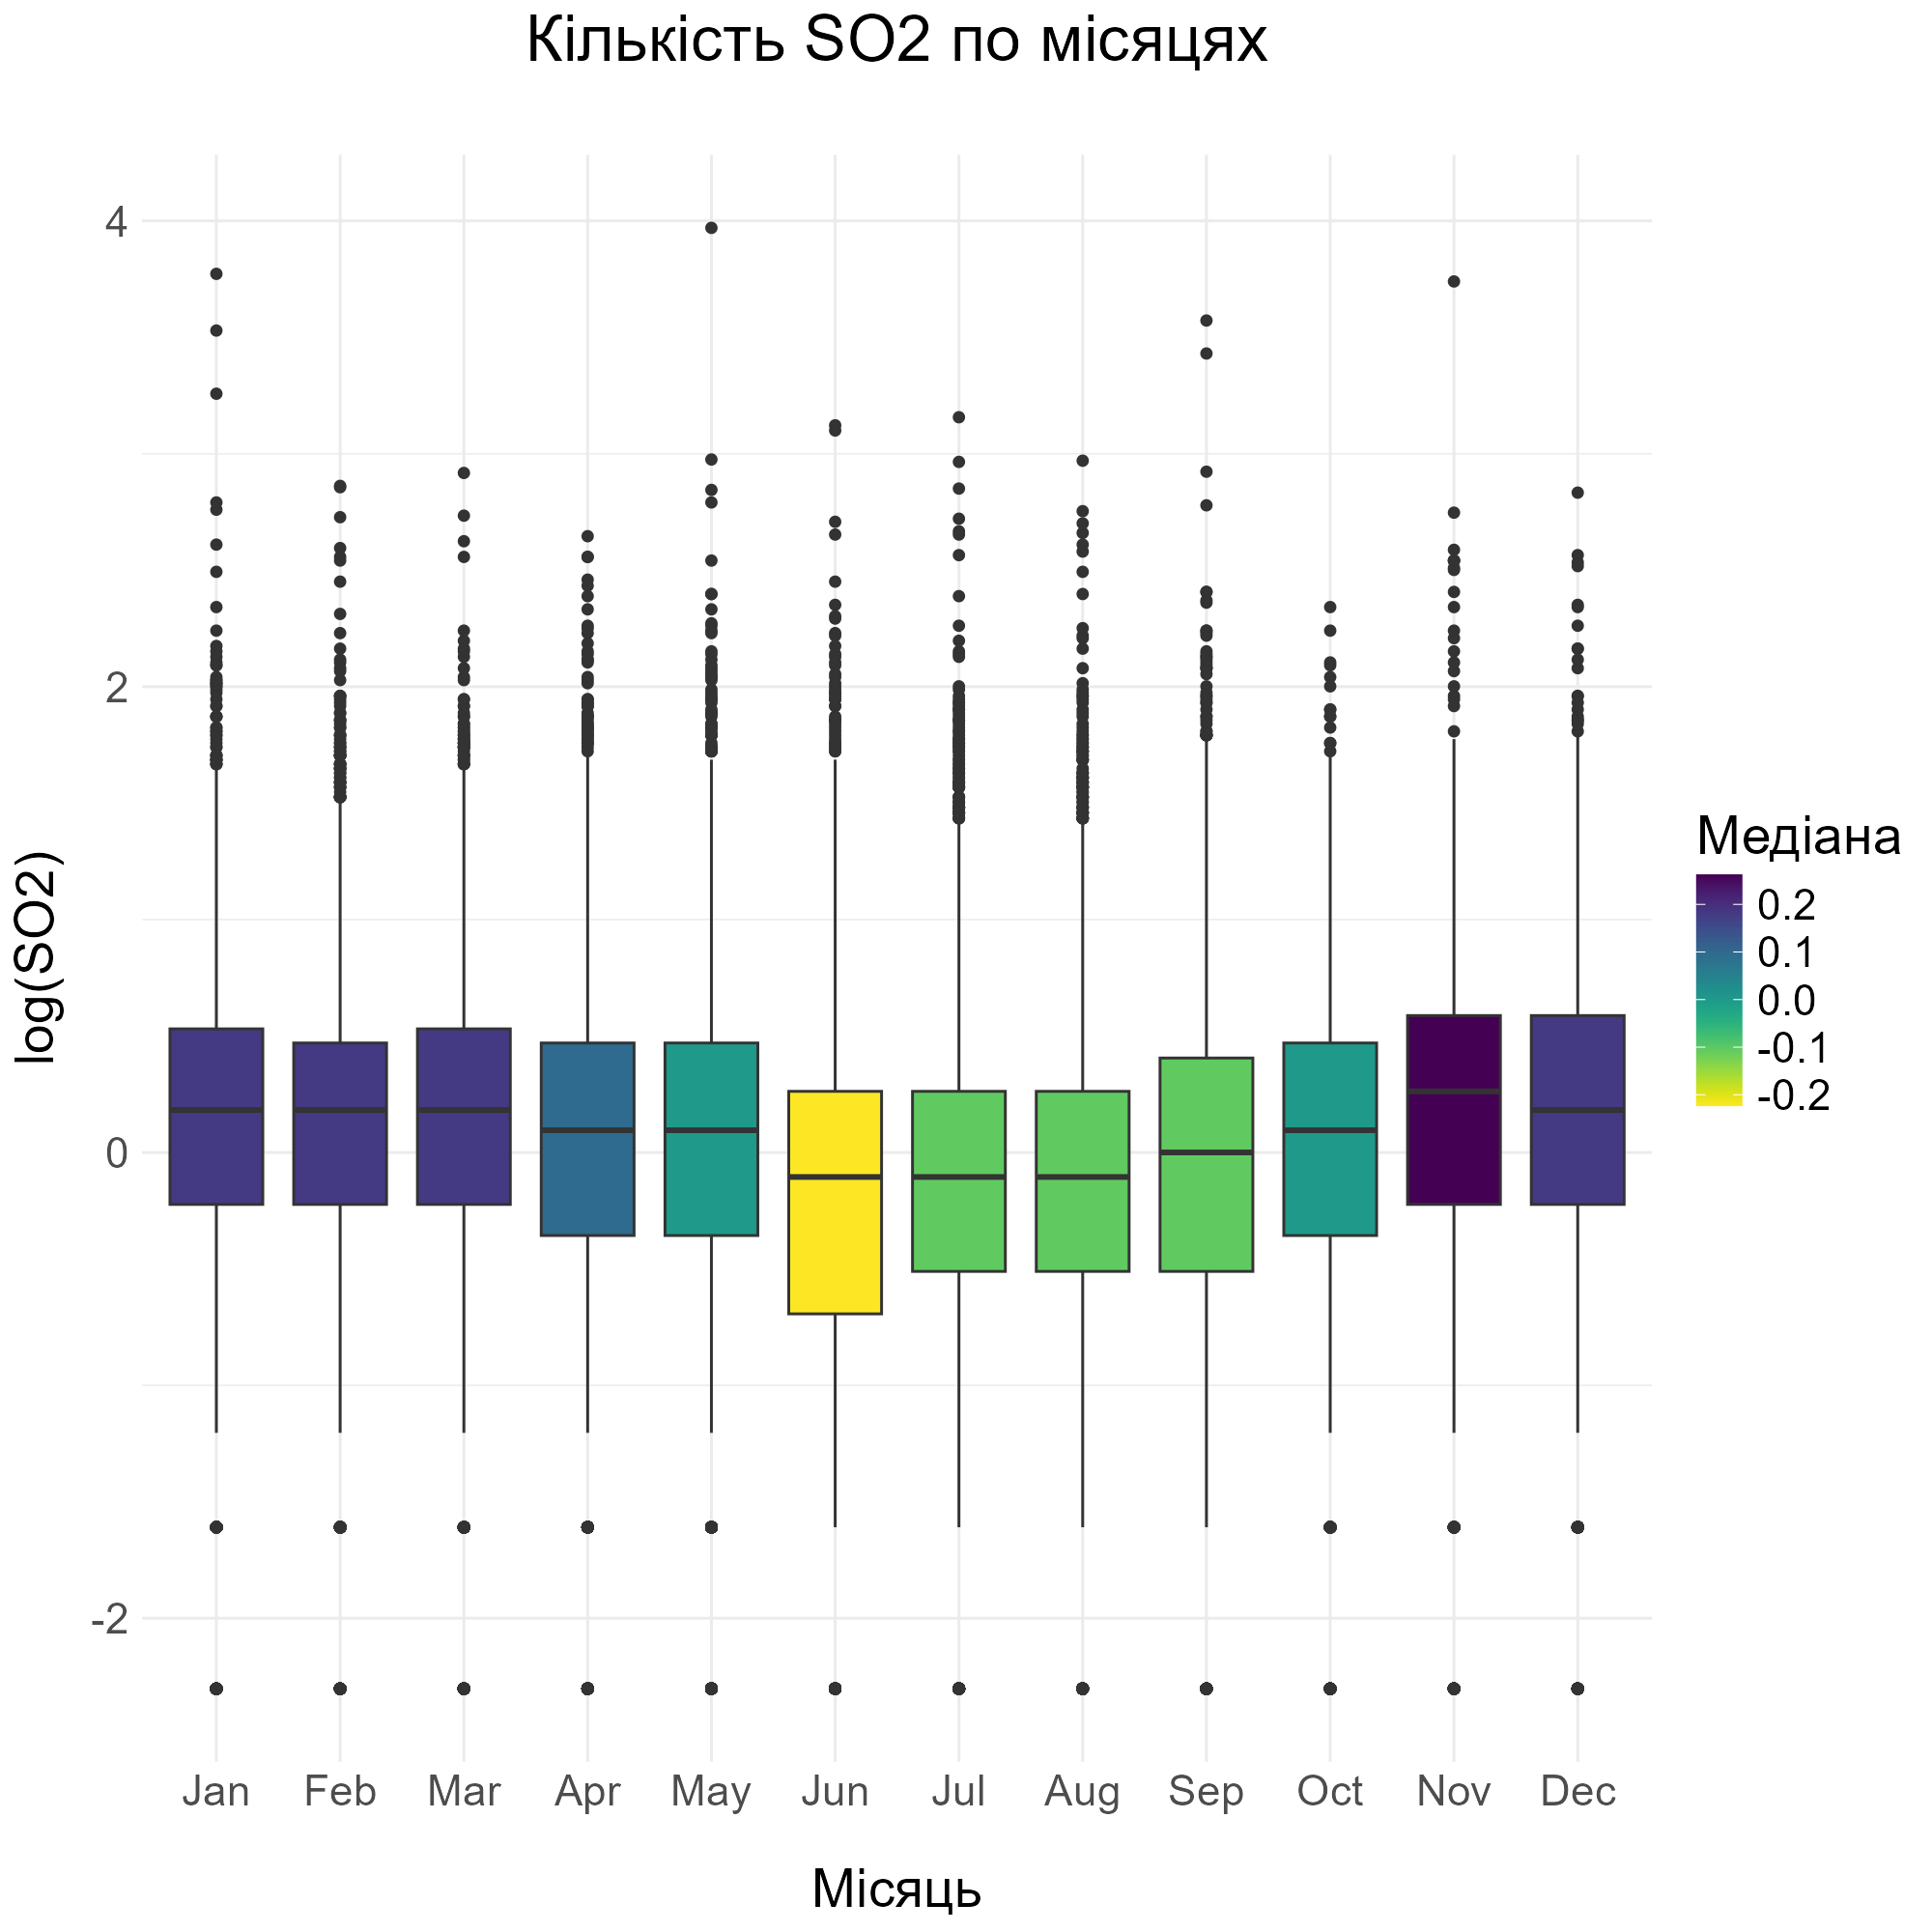
\includegraphics[width=\linewidth]{plots/question2/seasonal_so2.png}

  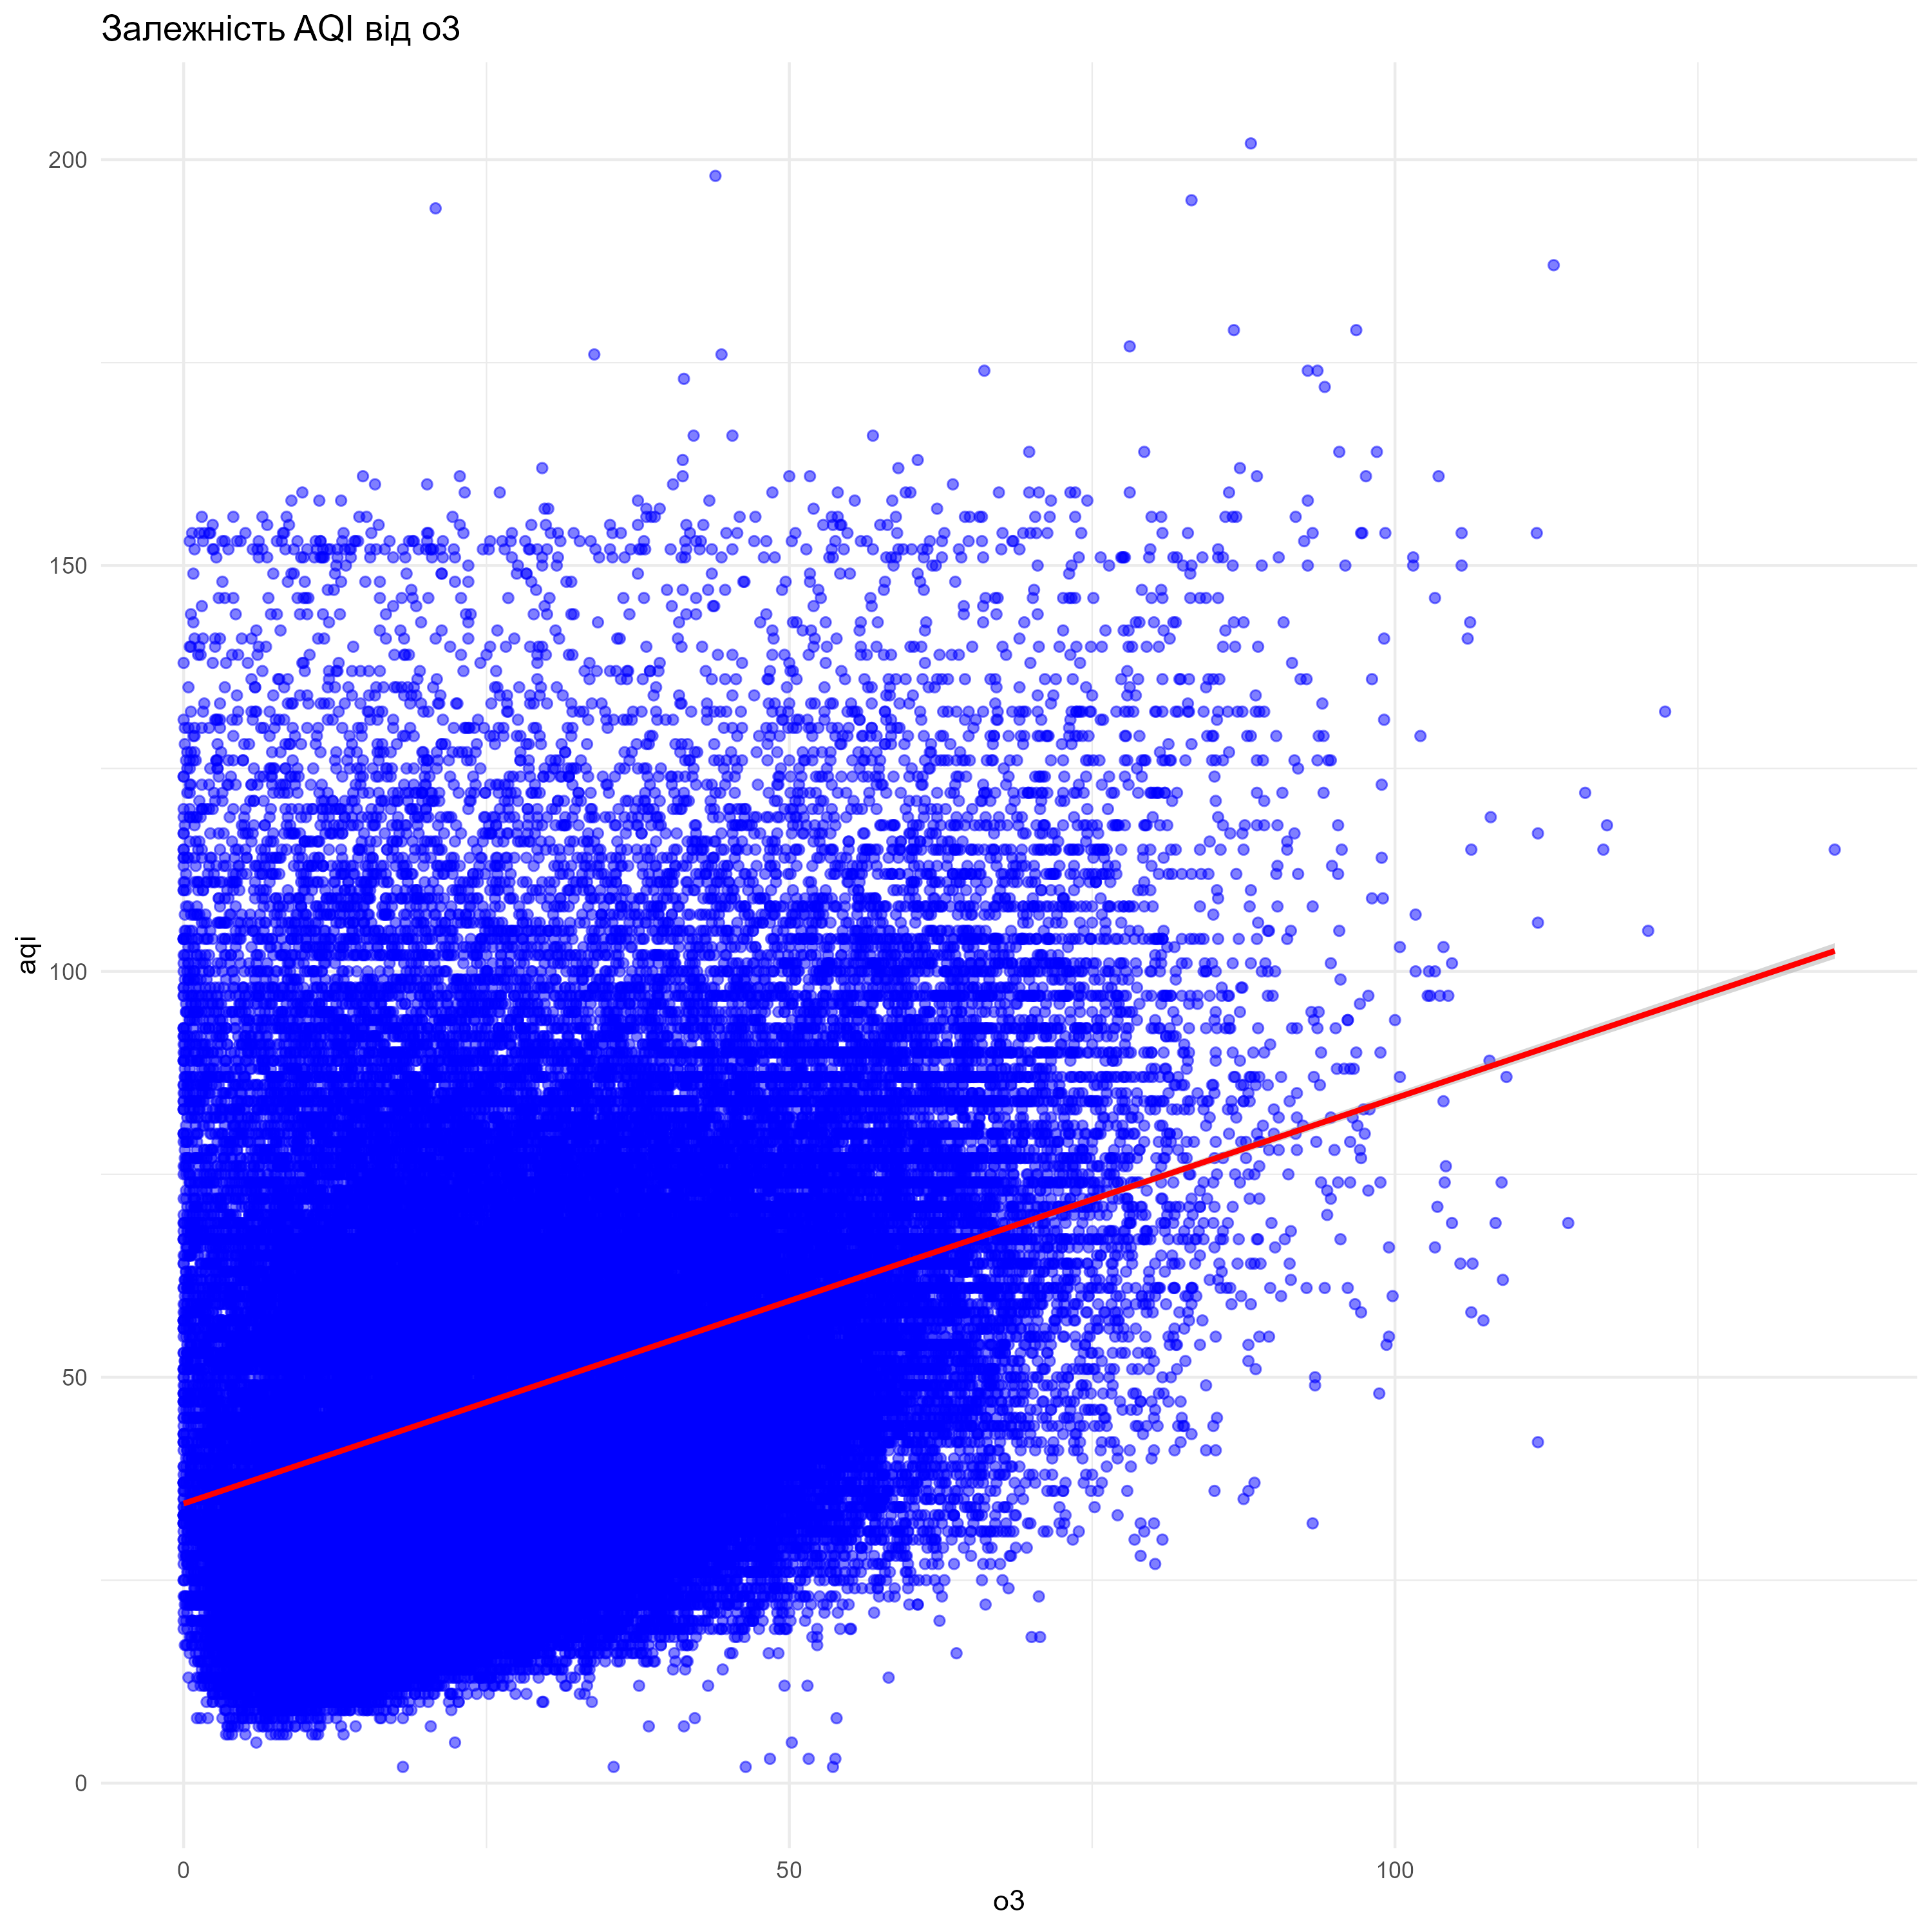
\includegraphics[width=\linewidth]{plots/question2/scatter_plot.png}

  \pagebreak

  \item Як змінюється якість повітря (status) протягом доби в різних районах?

  \quad \textit{Був використаний tidy набір даних}

  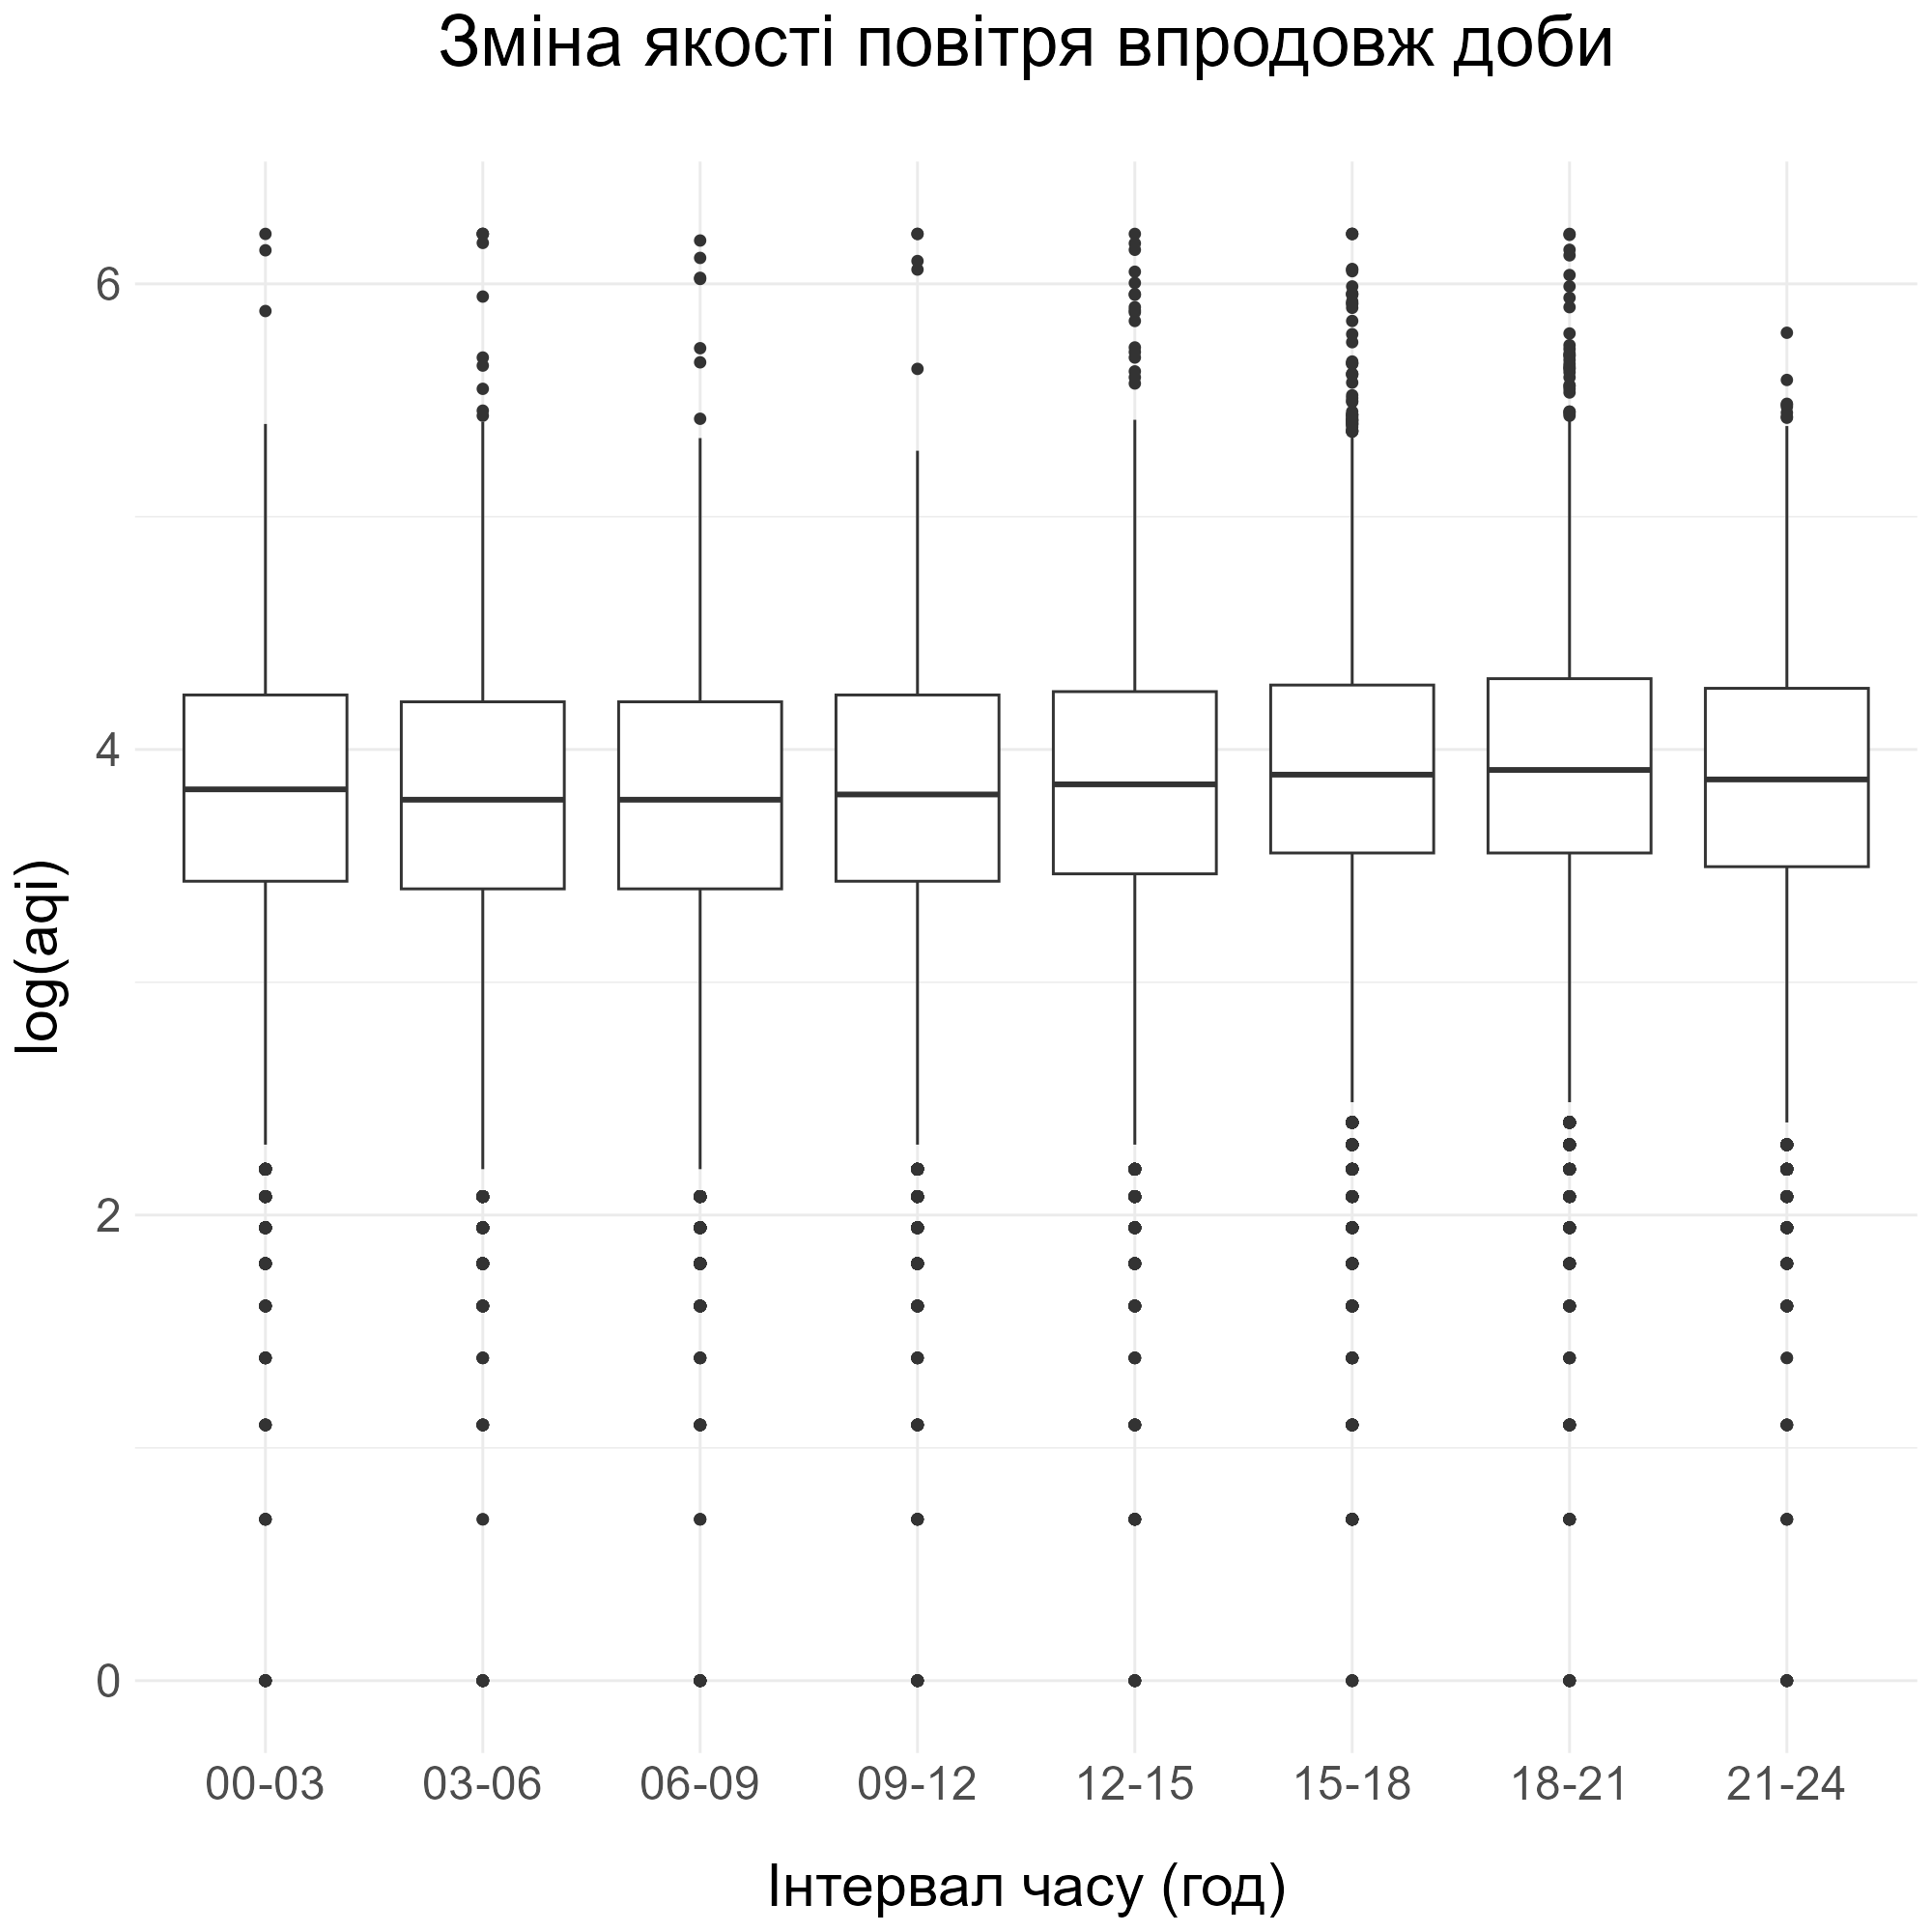
\includegraphics[width=\linewidth]{plots/question3/box.png}

  Аналізуючи даний графік, можна стведжувати, що якість повітря трохи
  покращується у другій половині дня.

  \pagebreak

  Також можемо розглянути детальніше регіони та зміни якости повітря.

  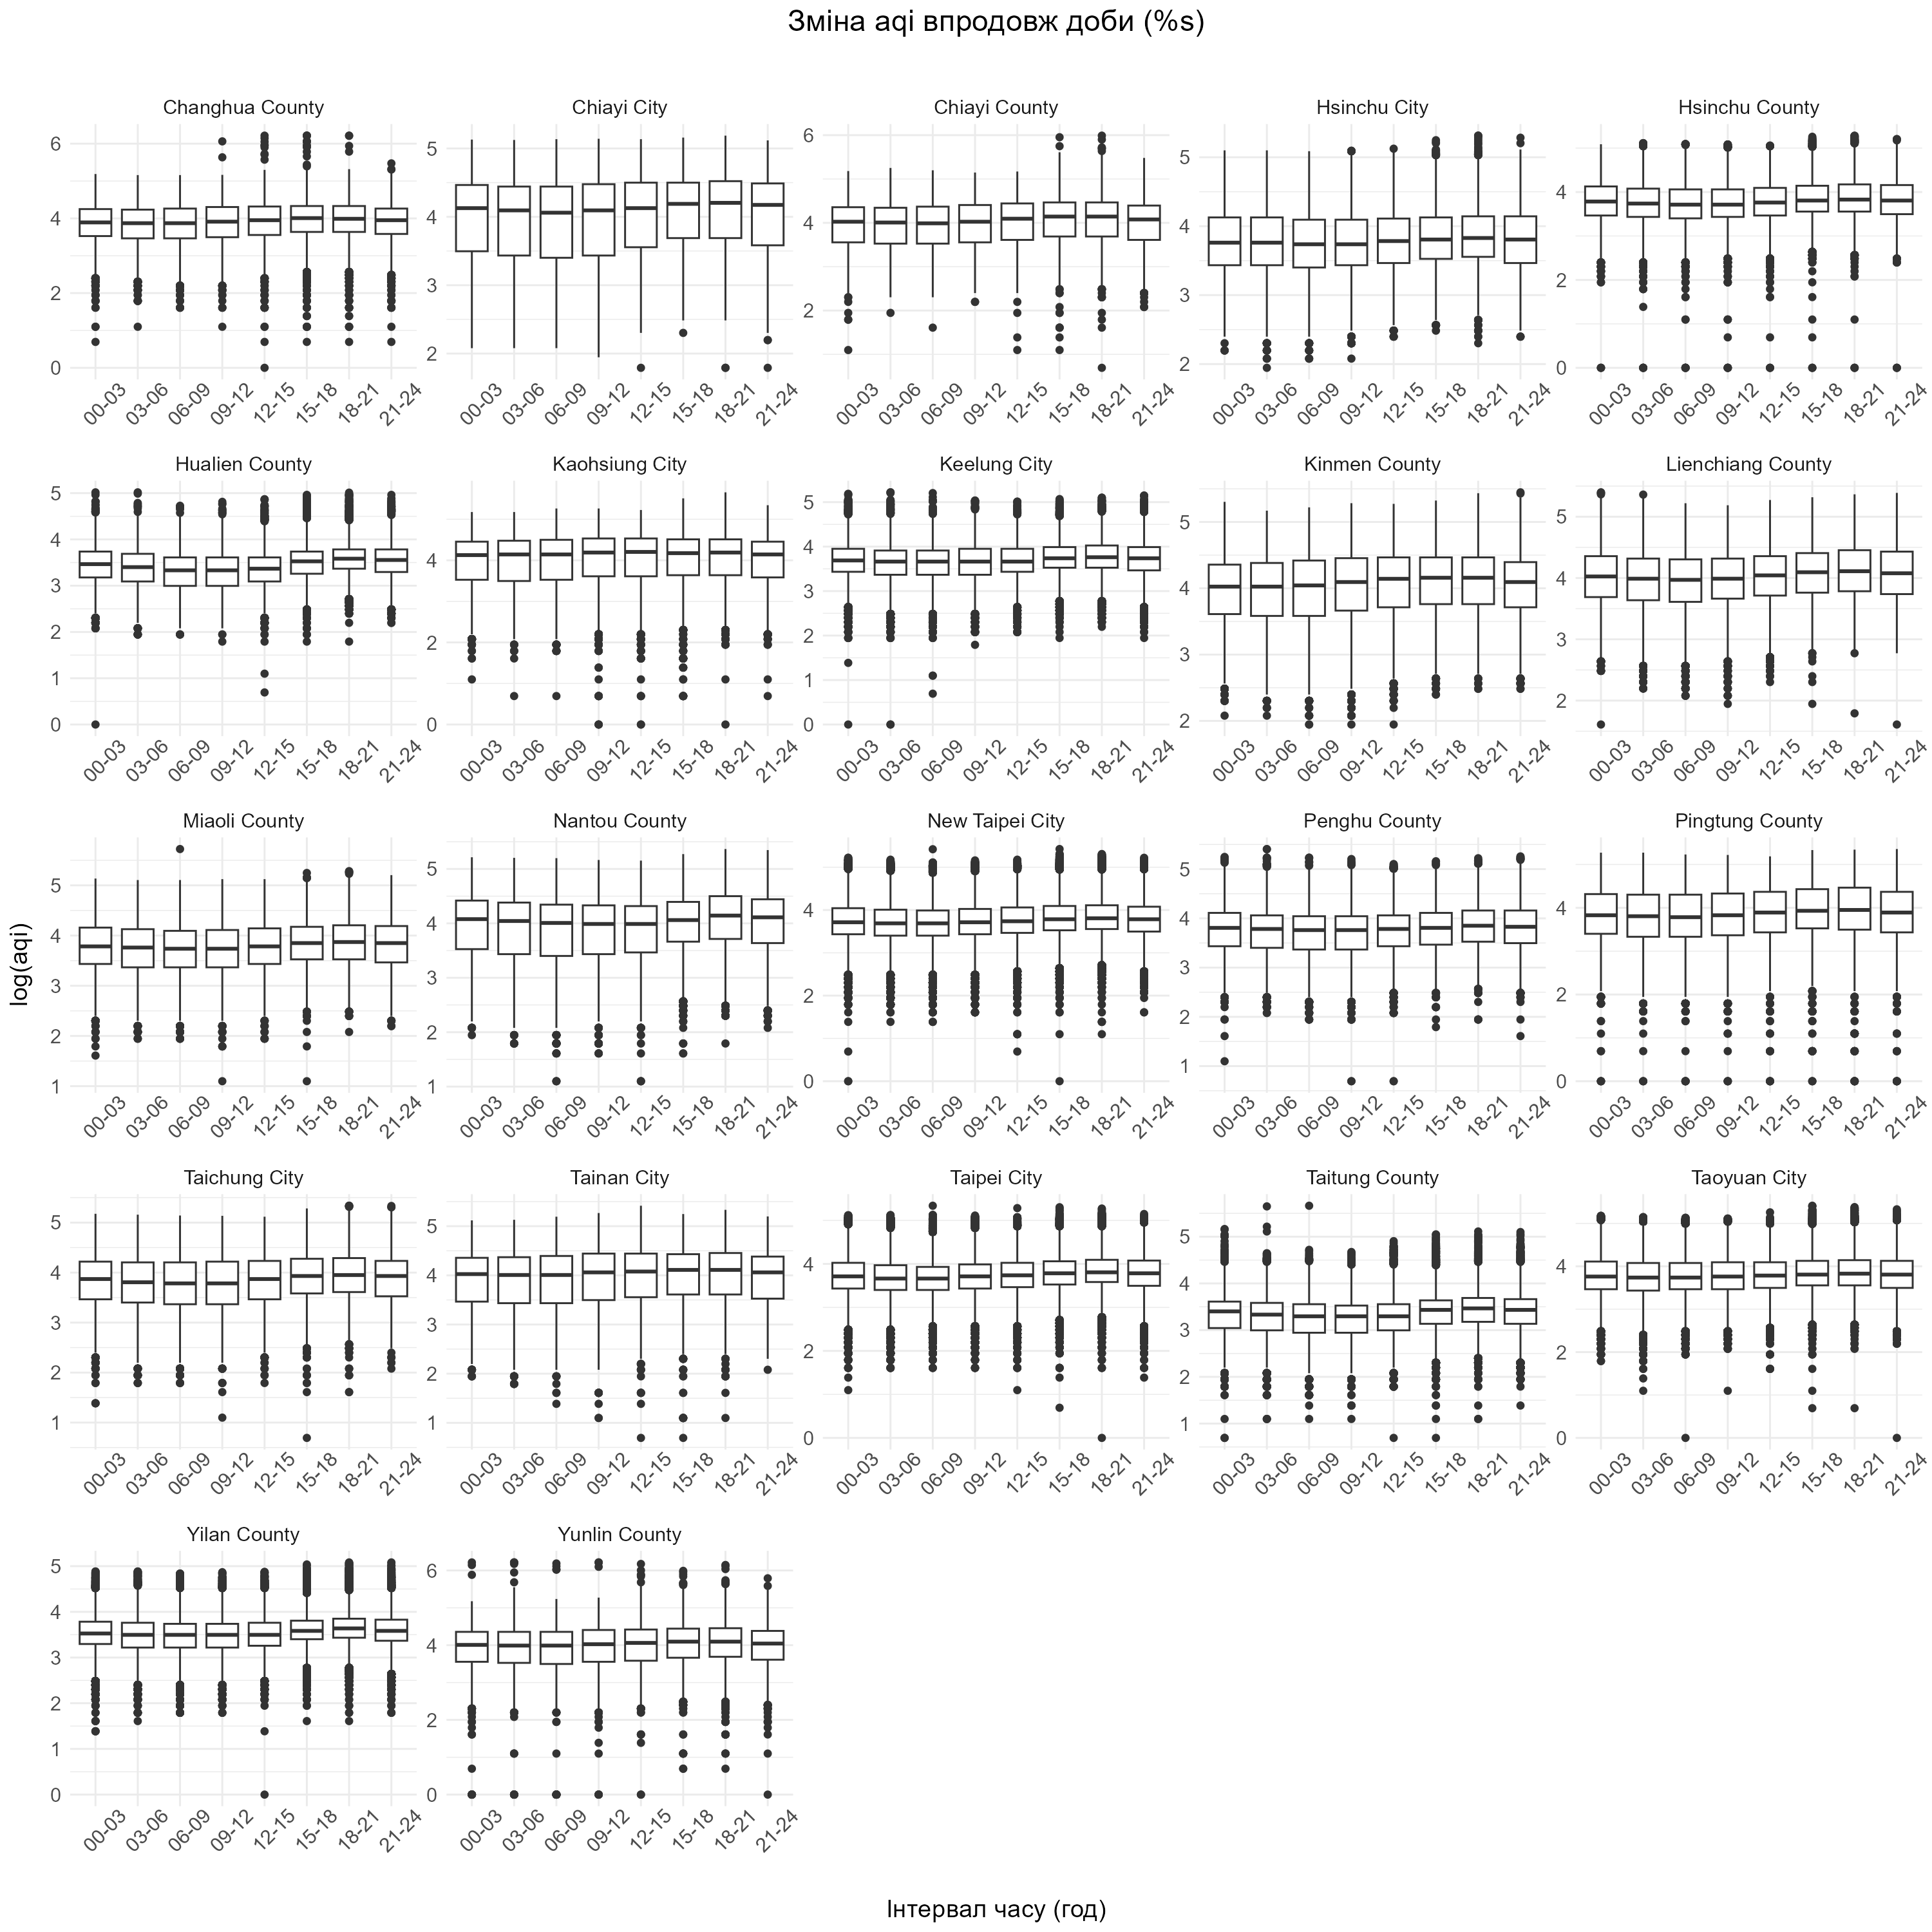
\includegraphics[width=\linewidth]{plots/question3/county-box.png}

  Бачимо, що зміна якости повітря в кожному регіоні не є суттєвою.

  \pagebreak

  \item Які регіони (county) мають найвищий середній рівень забруднення повітря (AQI) протягом року?

  \quad \textit{Був використаний trimmed набір даних}

  Всі наступні графіки, будуть будуватися на основі даних за 2016, 2017, 2023 та 2024 роки.

  Для розуміння числових даних, розглянемо 10 регіонів з найвищим рівнем AQI за відповідні роки.

  \begin{tabular}{ccc}
    \textbf{Year} & \textbf{Сounty} & \textbf{Average AQI} \\
    2016 & Chiayi City     & 120.31 \\
    2016 & Kaohsiung City  & 112.10 \\
    2016 & Tainan City     & 99.60  \\
    2016 & Pingtung County & 97.15  \\
    2016 & Yunlin County   & 91.23  \\
    2016 & Chiayi County   & 88.83  \\
    2016 & Nantou County   & 83.34  \\
    2016 & Changhua County & 81.68  \\
    2016 & Kinmen County   & 81.60  \\
    2016 & Taichung City   & 77.96  \\
  \end{tabular}

  Візуалізуючи отримуємо наступне:

  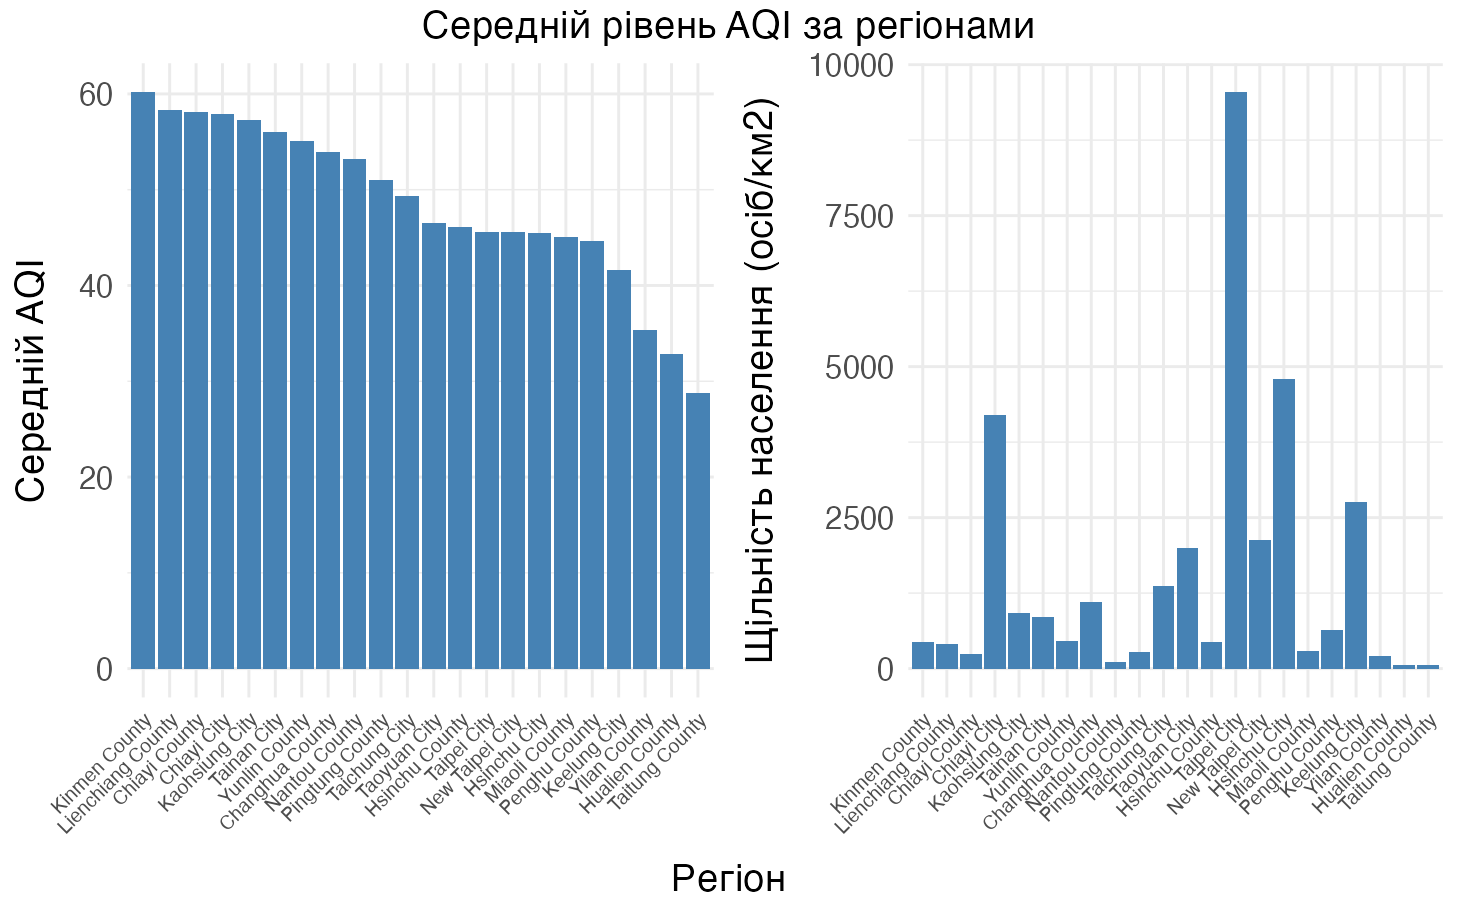
\includegraphics[width=\linewidth]{plots/question4/avg_aqi_by_county_w_dens.png}

  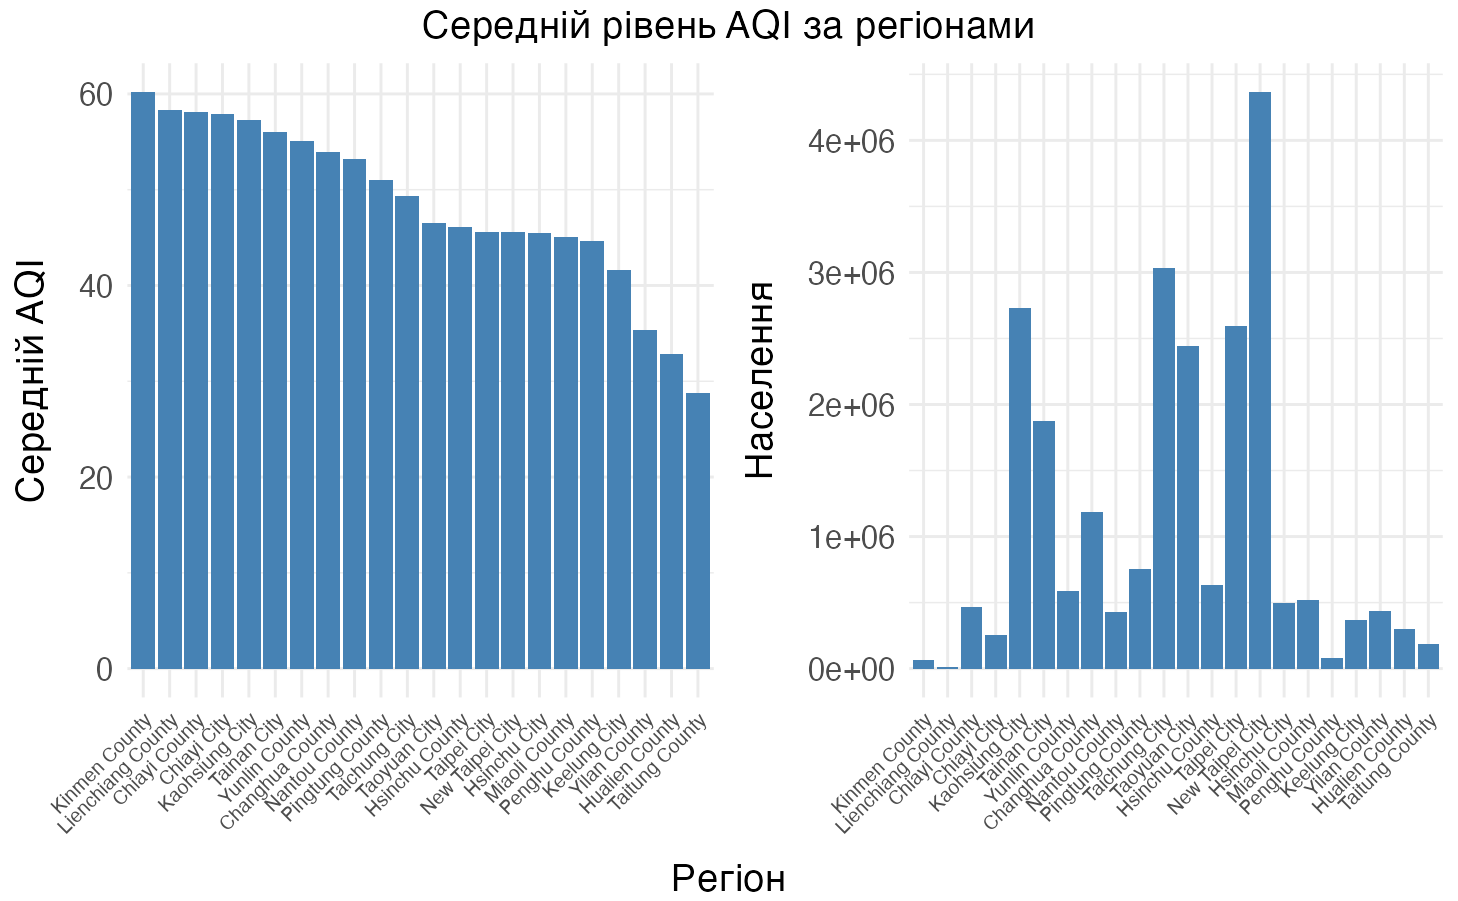
\includegraphics[width=\linewidth]{plots/question4/avg_aqi_by_county_w_pop.png}

  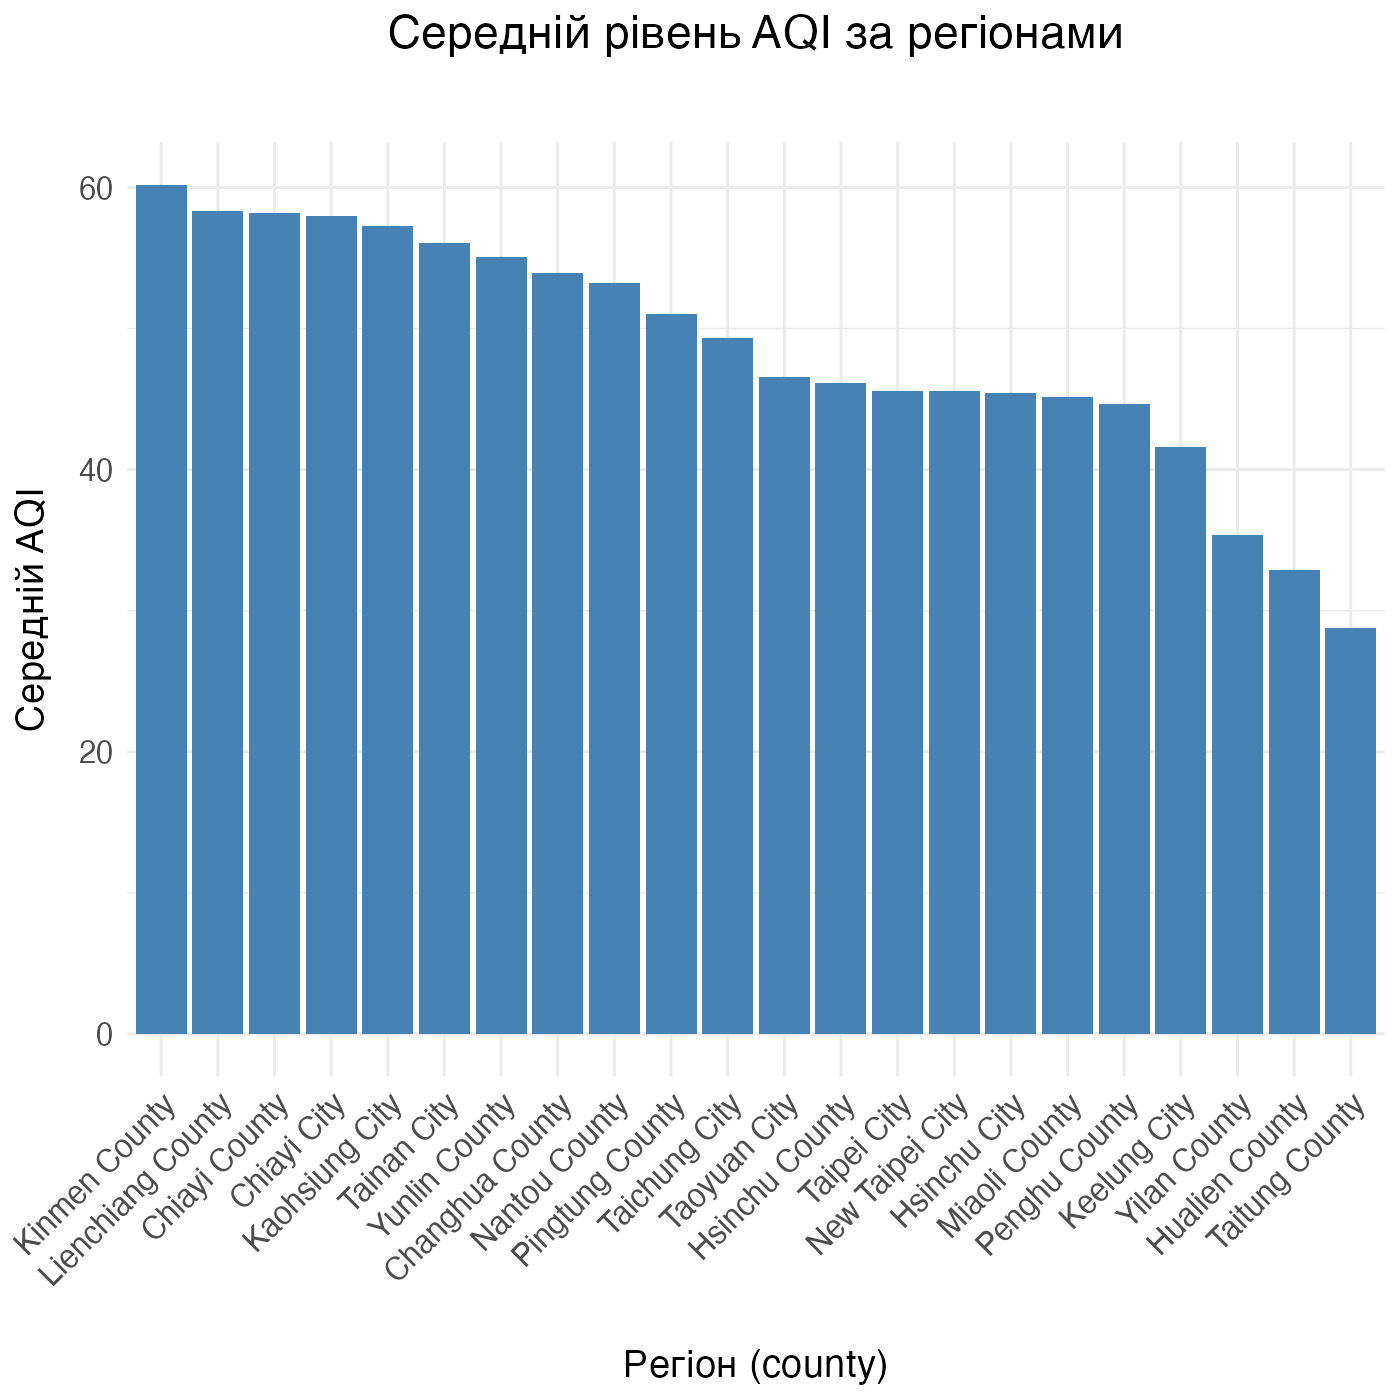
\includegraphics[width=\linewidth]{plots/question4/avg_aqi_by_county.png}

  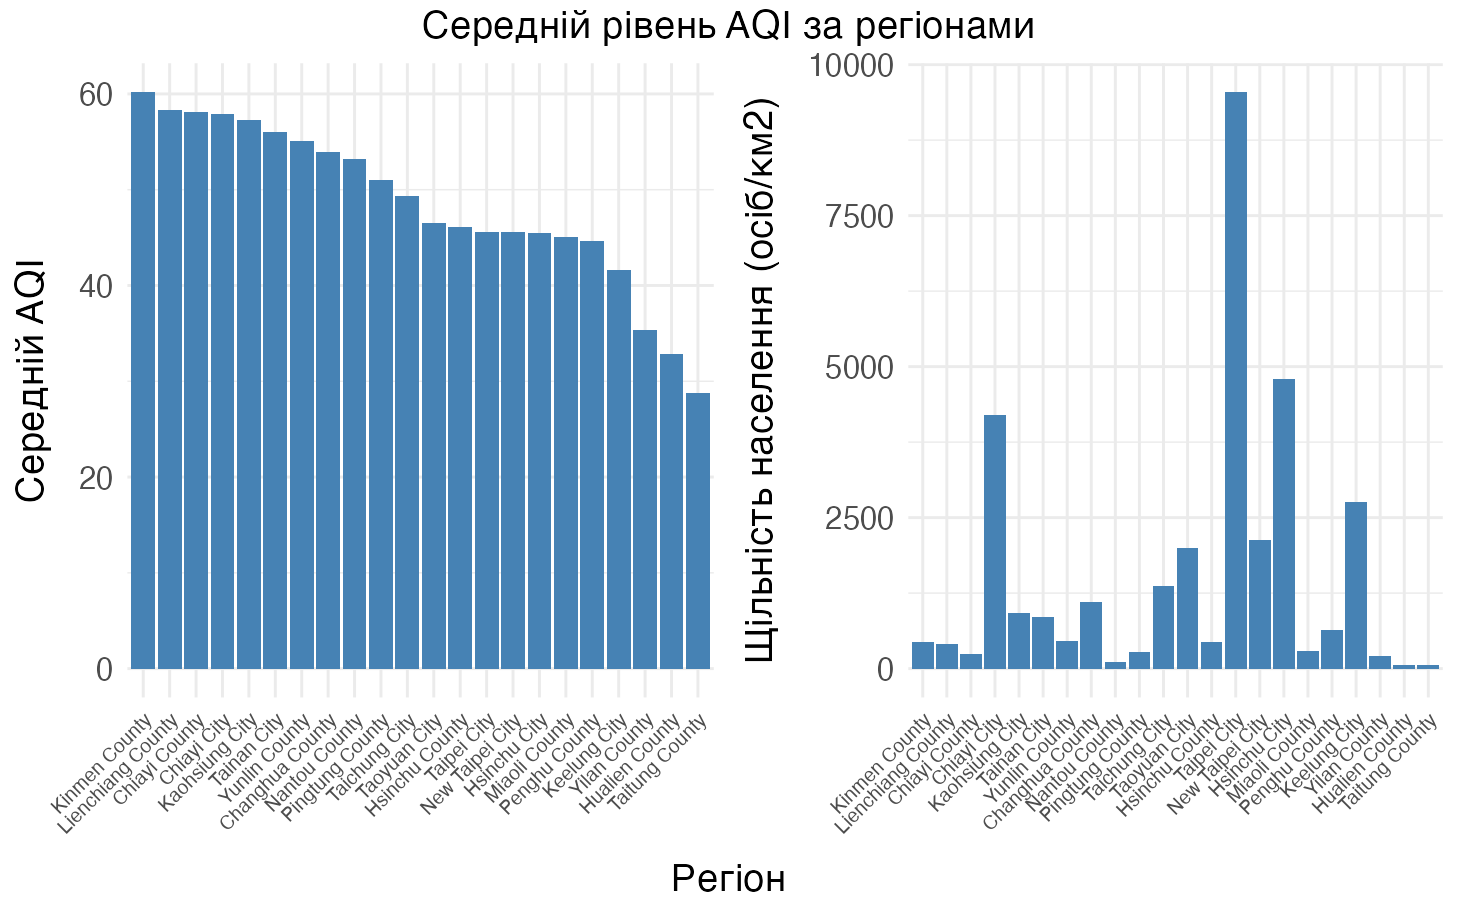
\includegraphics[width=\linewidth]{plots/question4/avg_aqi_by_county_w_dens.png}

  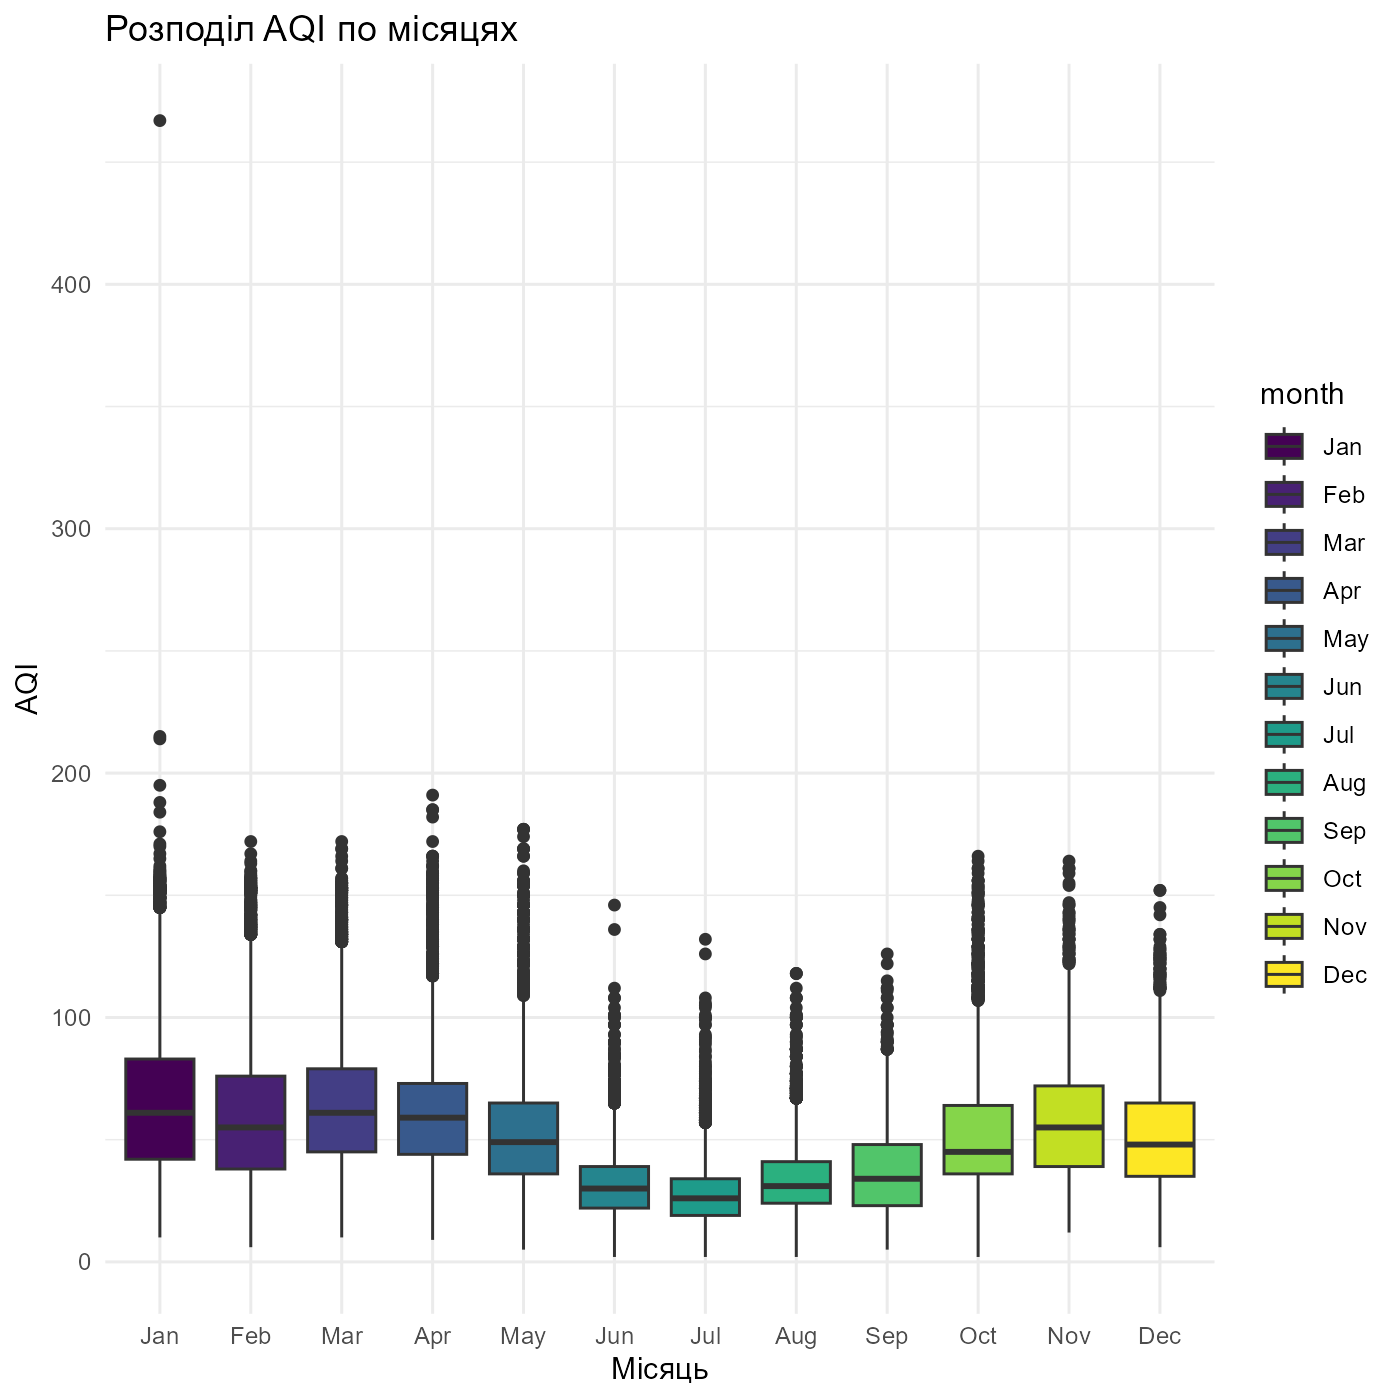
\includegraphics[width=\linewidth]{plots/question4/seasonal_change.png}

  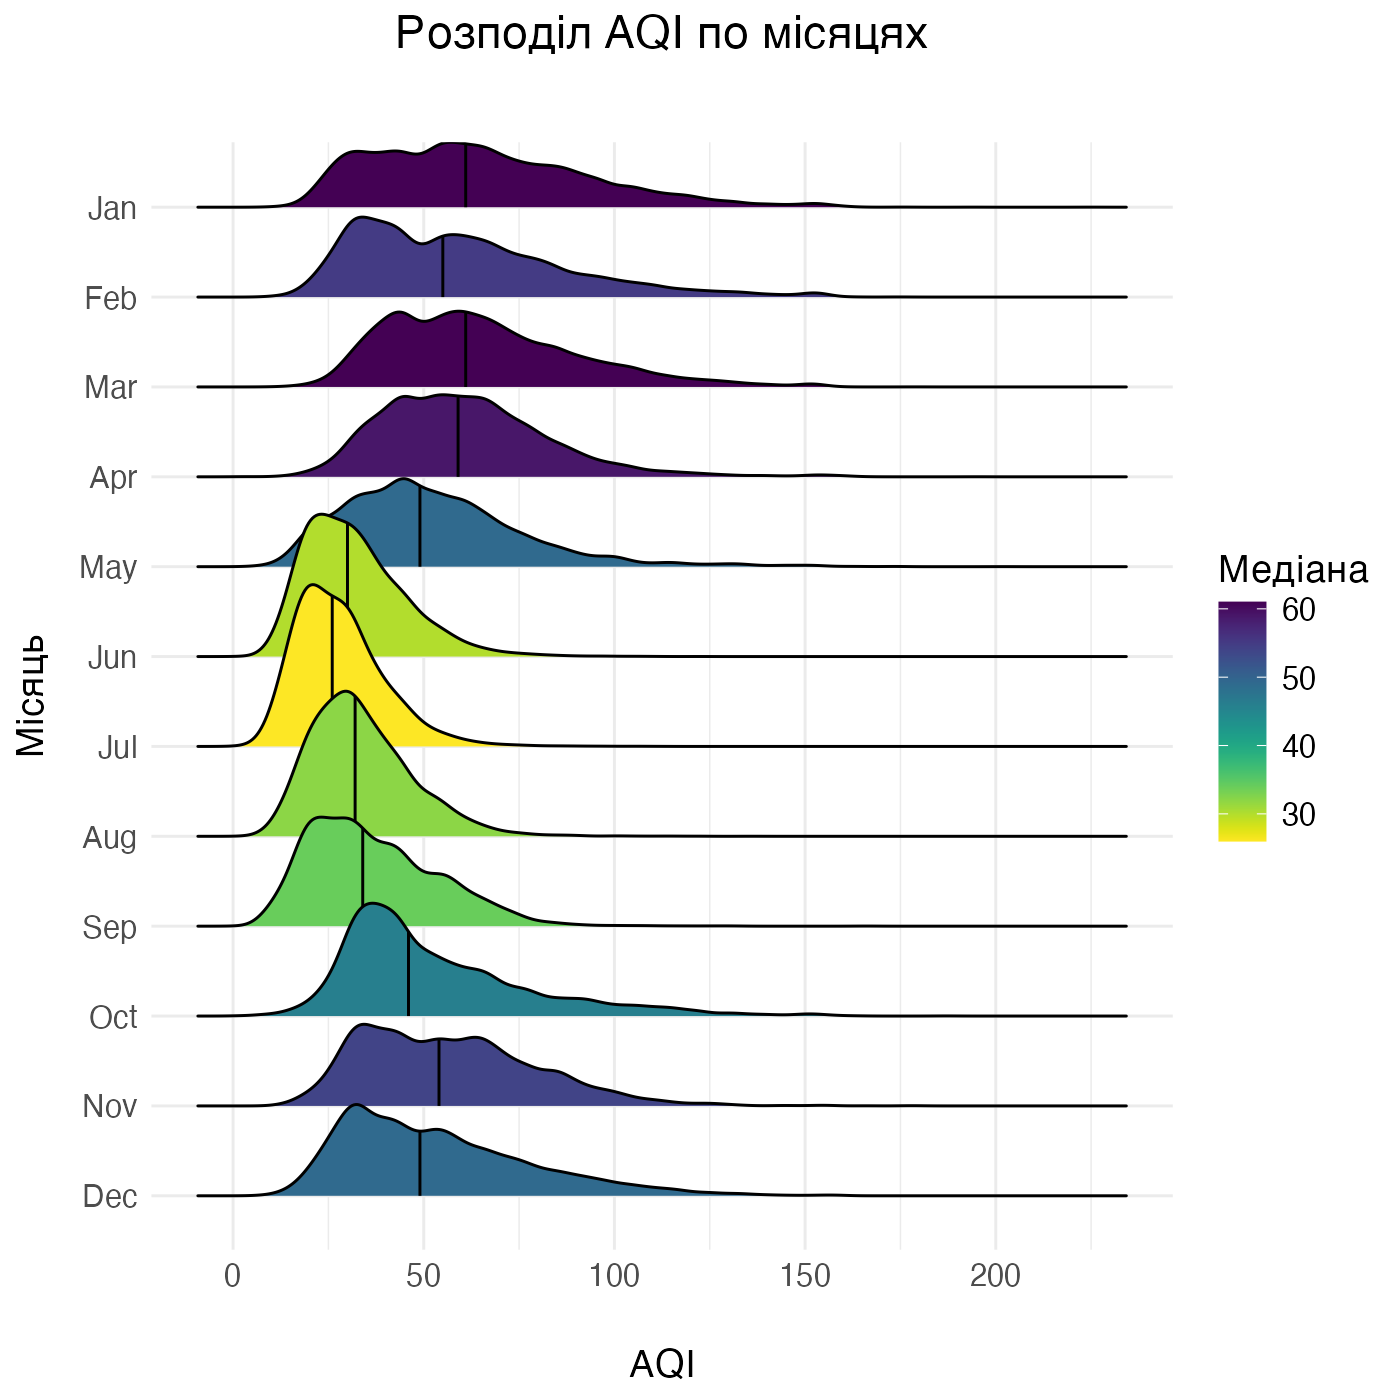
\includegraphics[width=\linewidth]{plots/question4/seasonal_change_ridgeline.png}

  \pagebreak

  \item Як змінився загальний рівень забруднення по регіонам після початку реформи?

  \quad \textit{Був використаний tidy набір даних}

  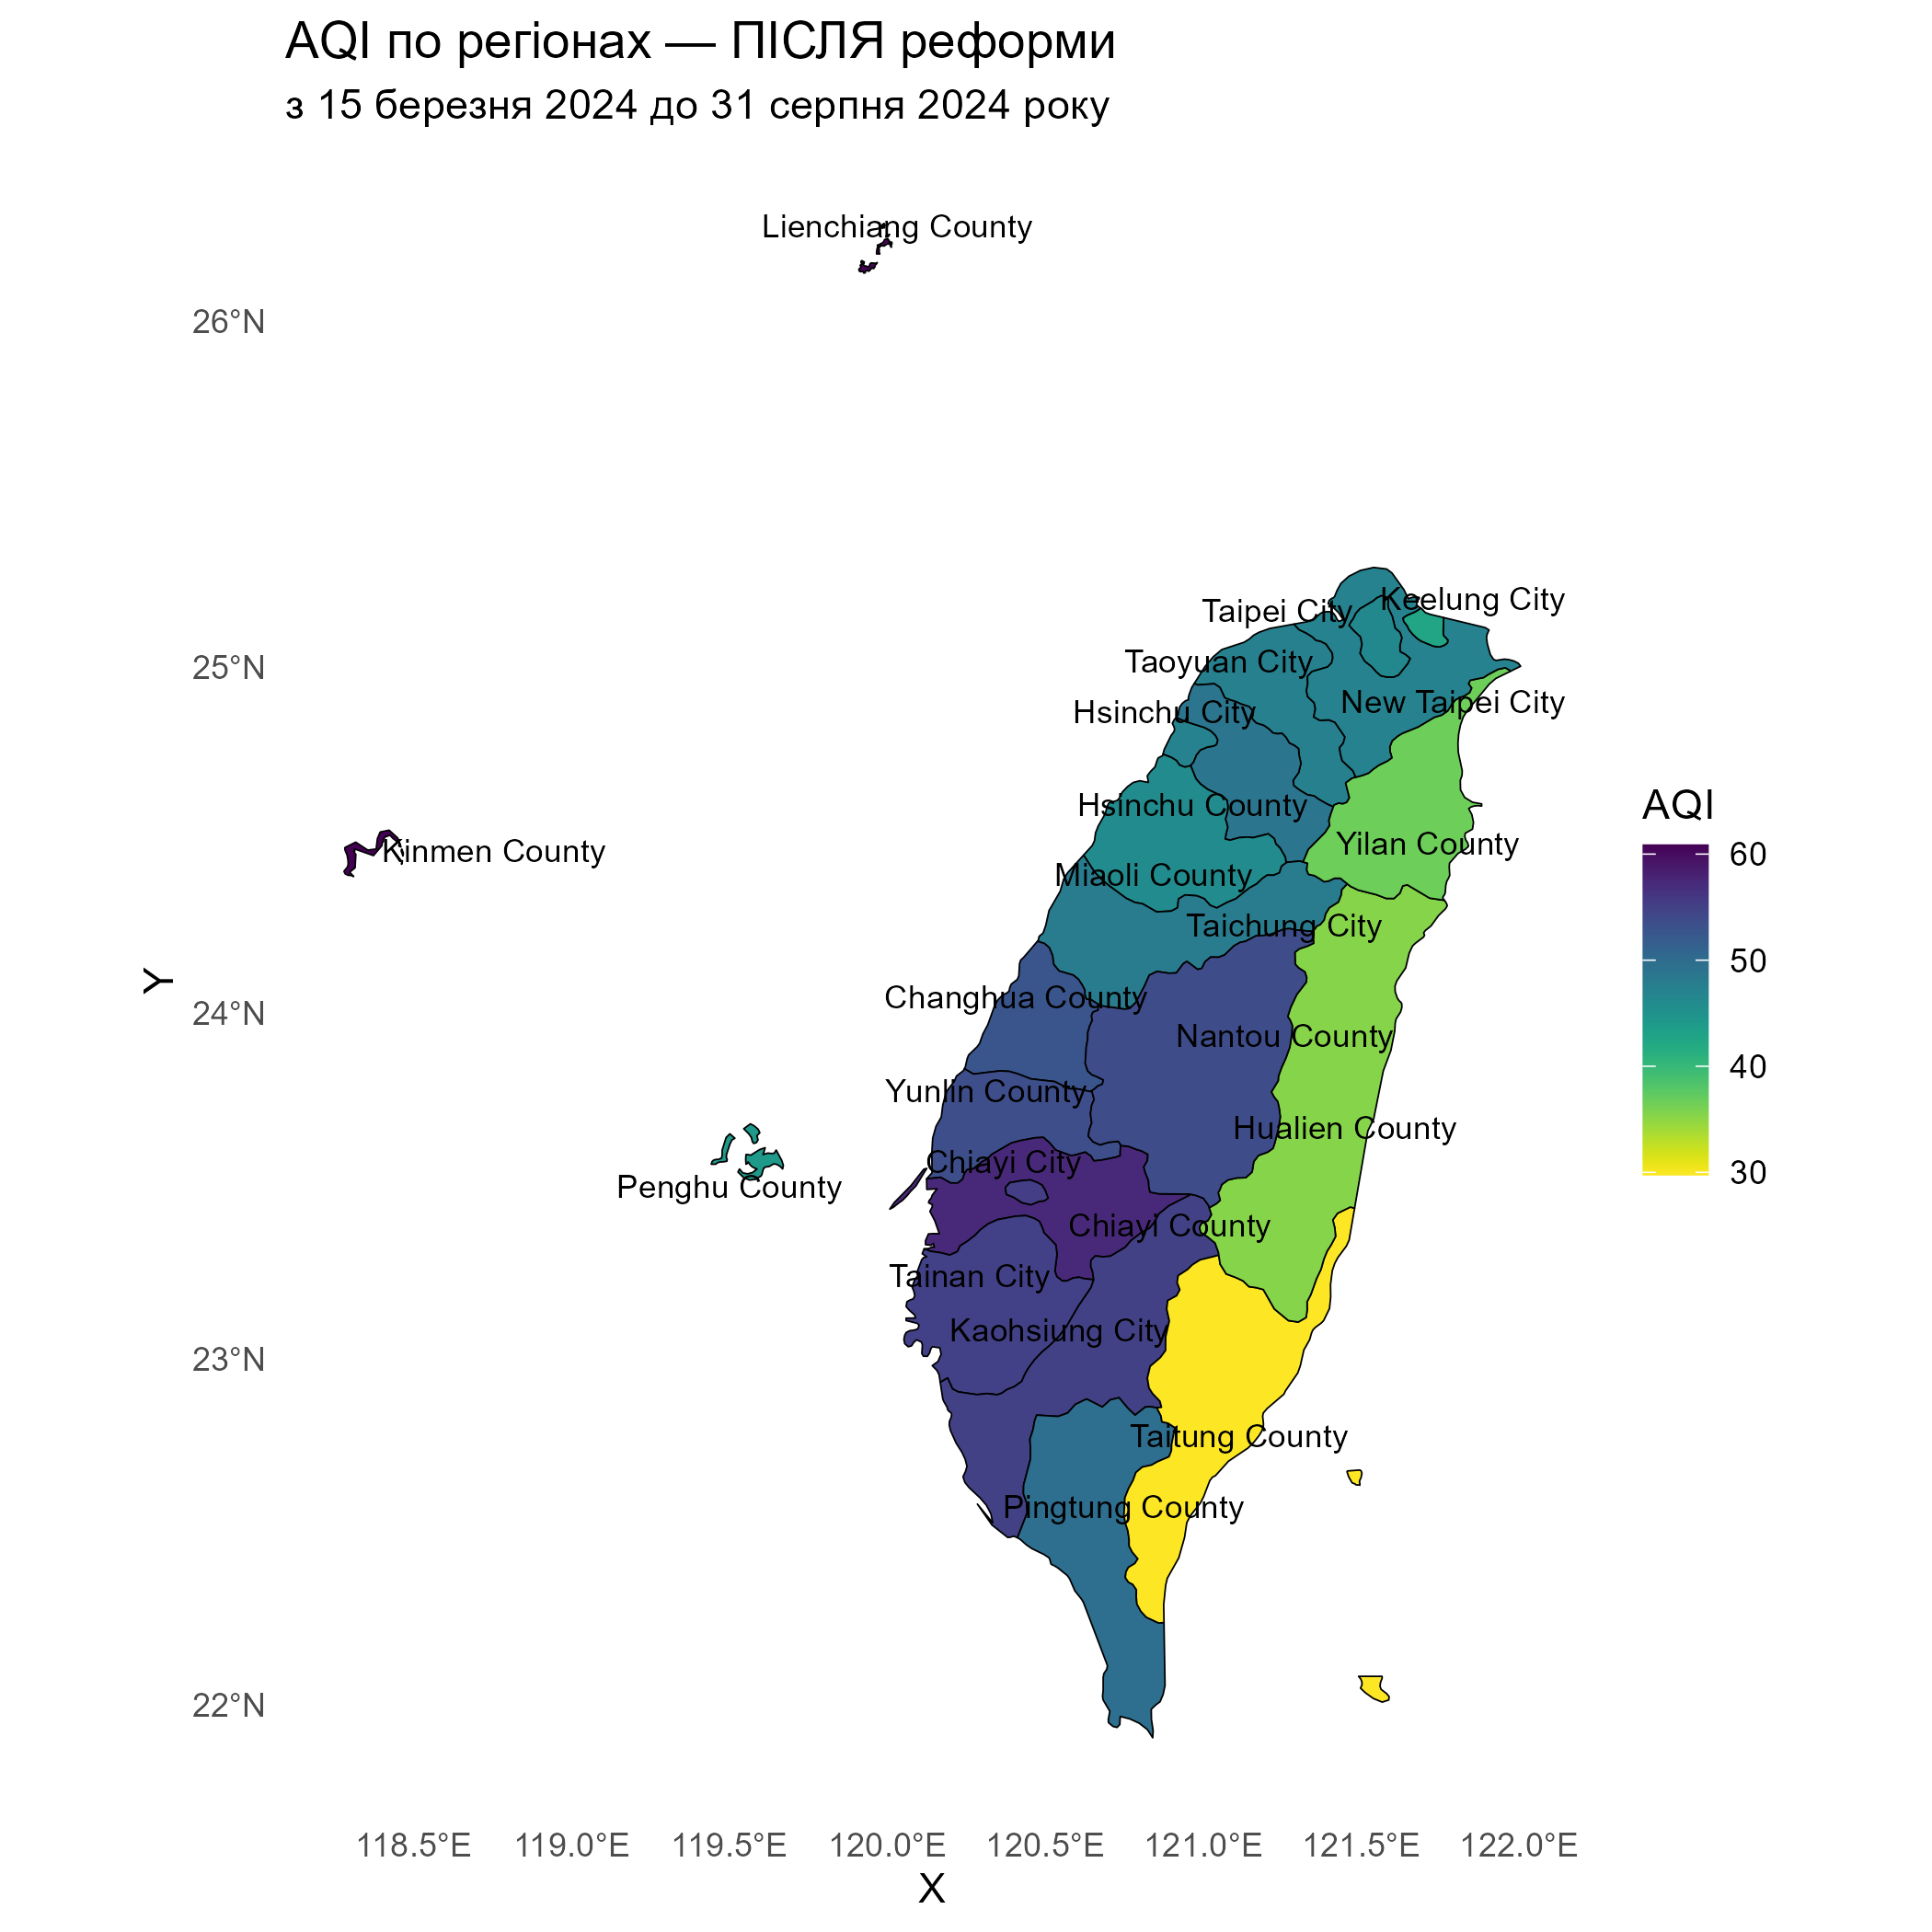
\includegraphics[width=\linewidth]{plots/question5/map_after_reform.png}
  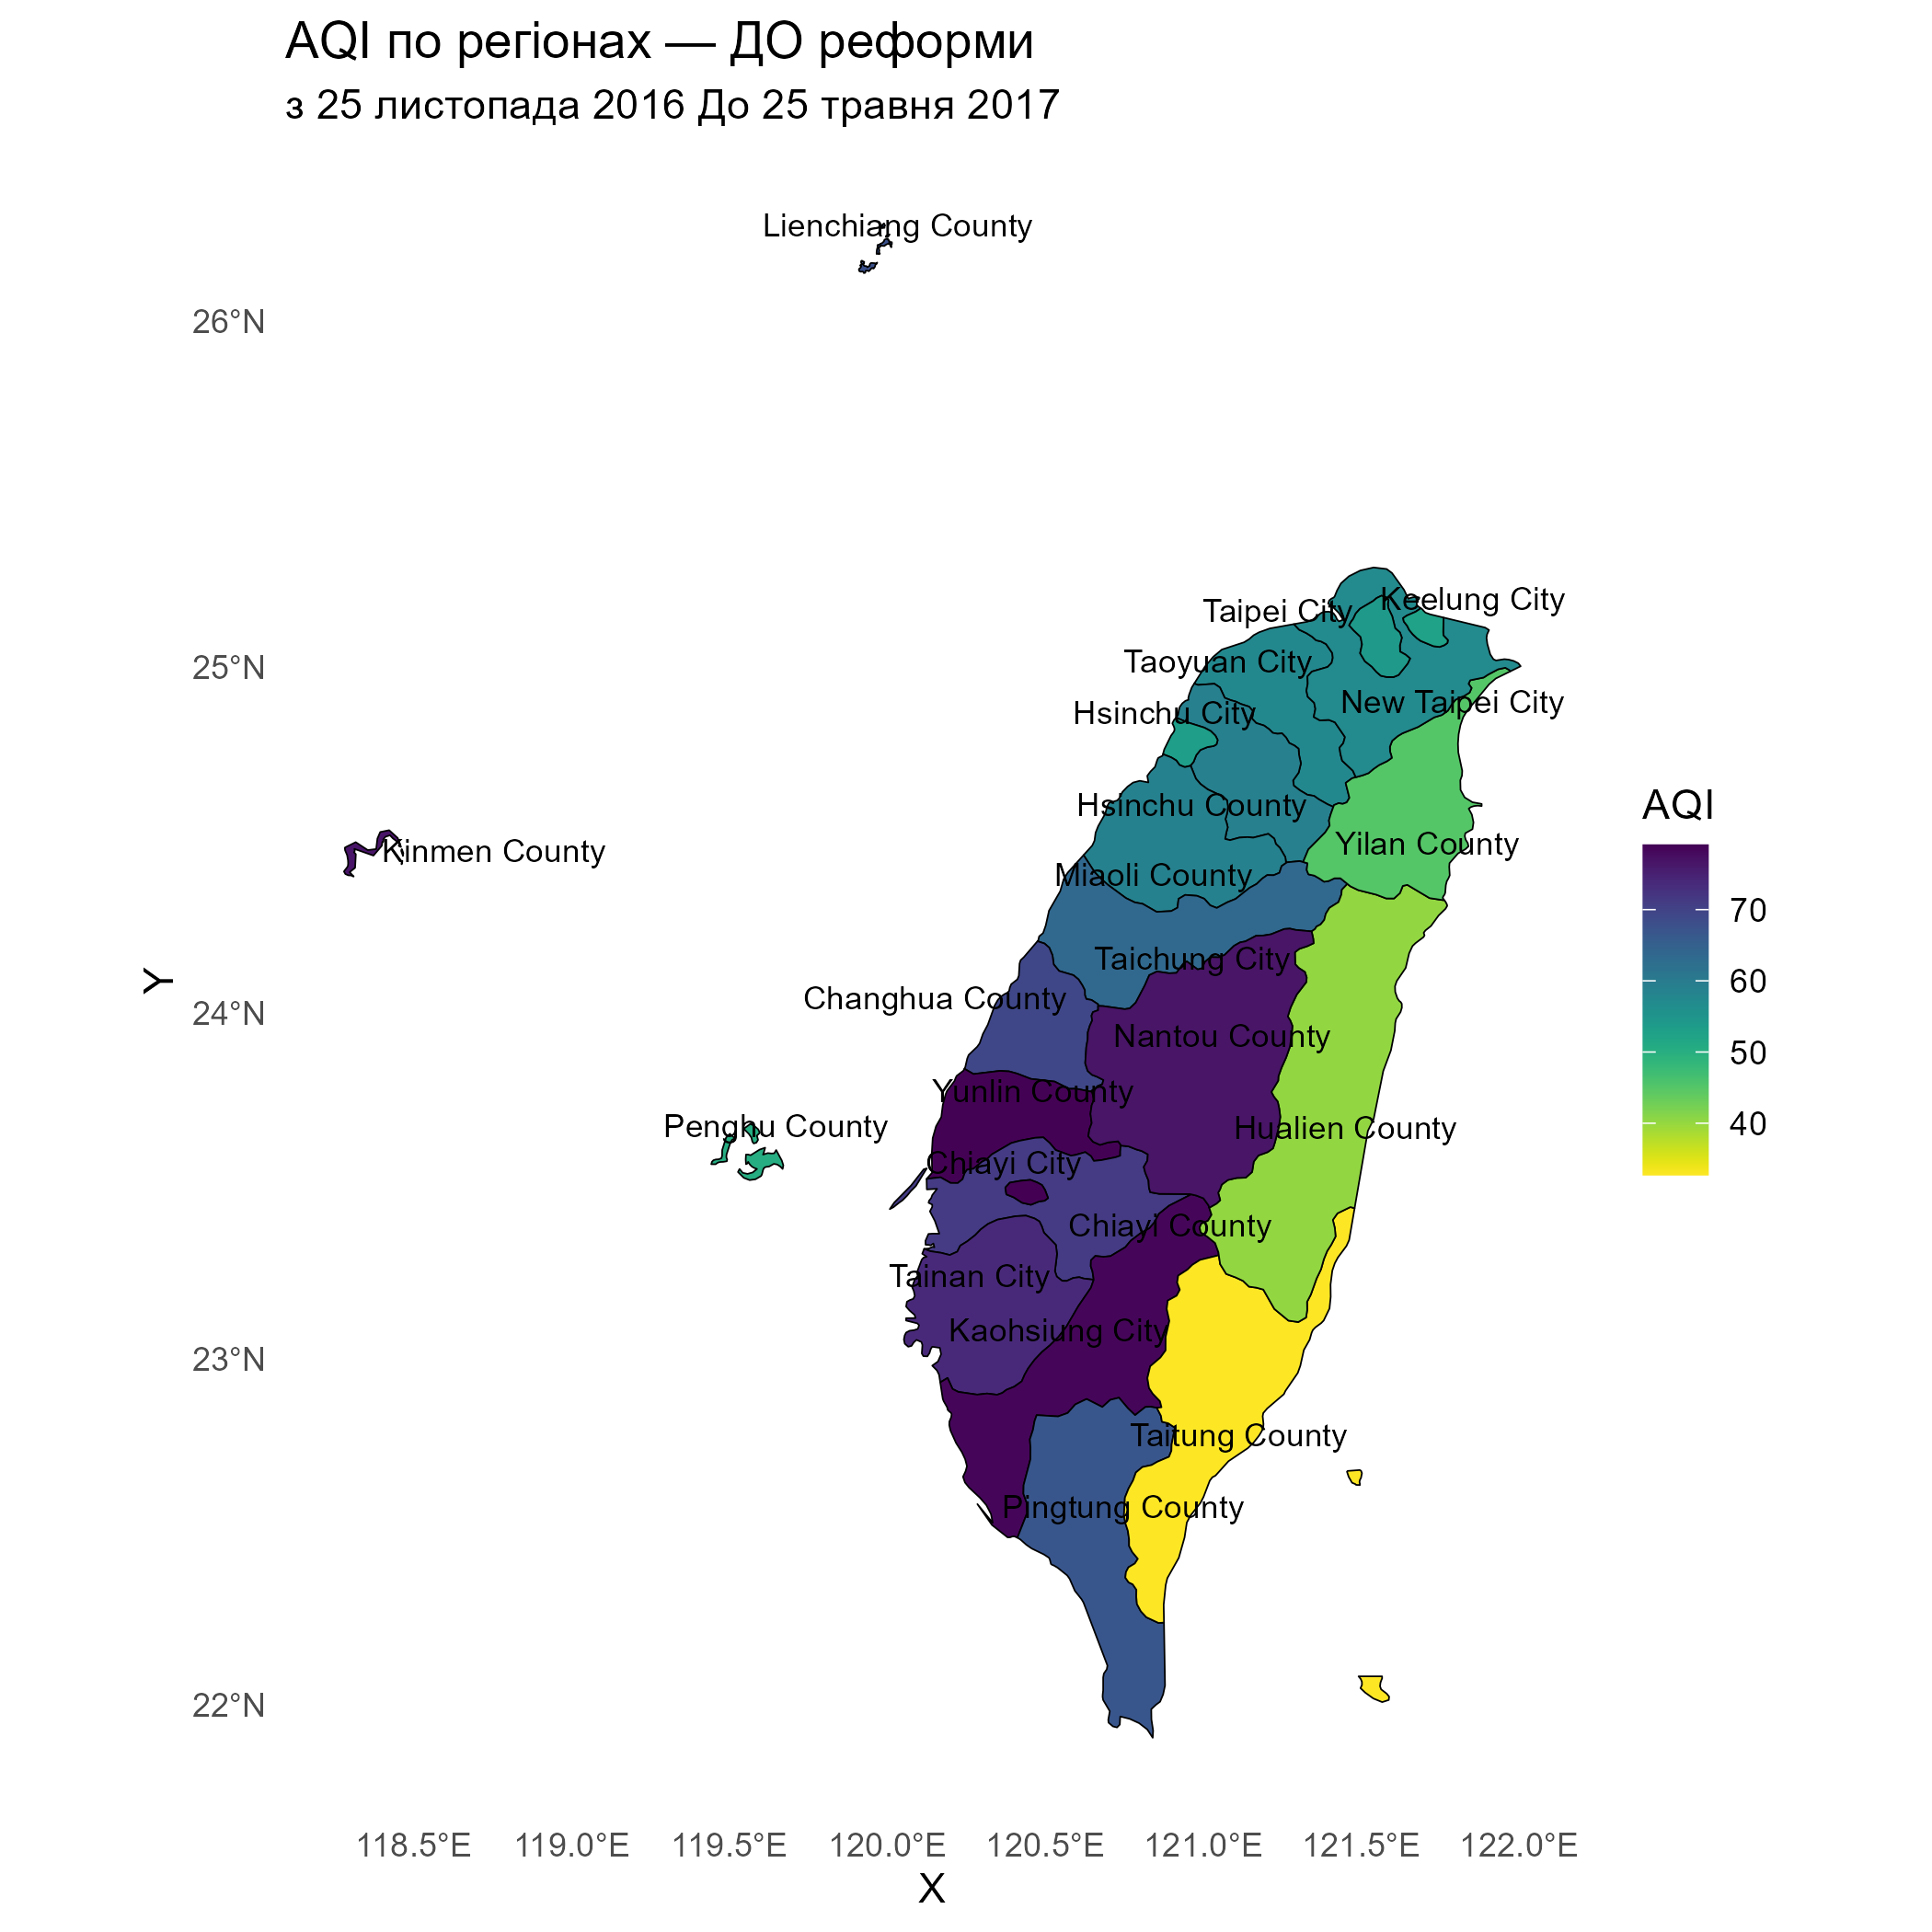
\includegraphics[width=\linewidth]{plots/question5/map_before_reform.png}
  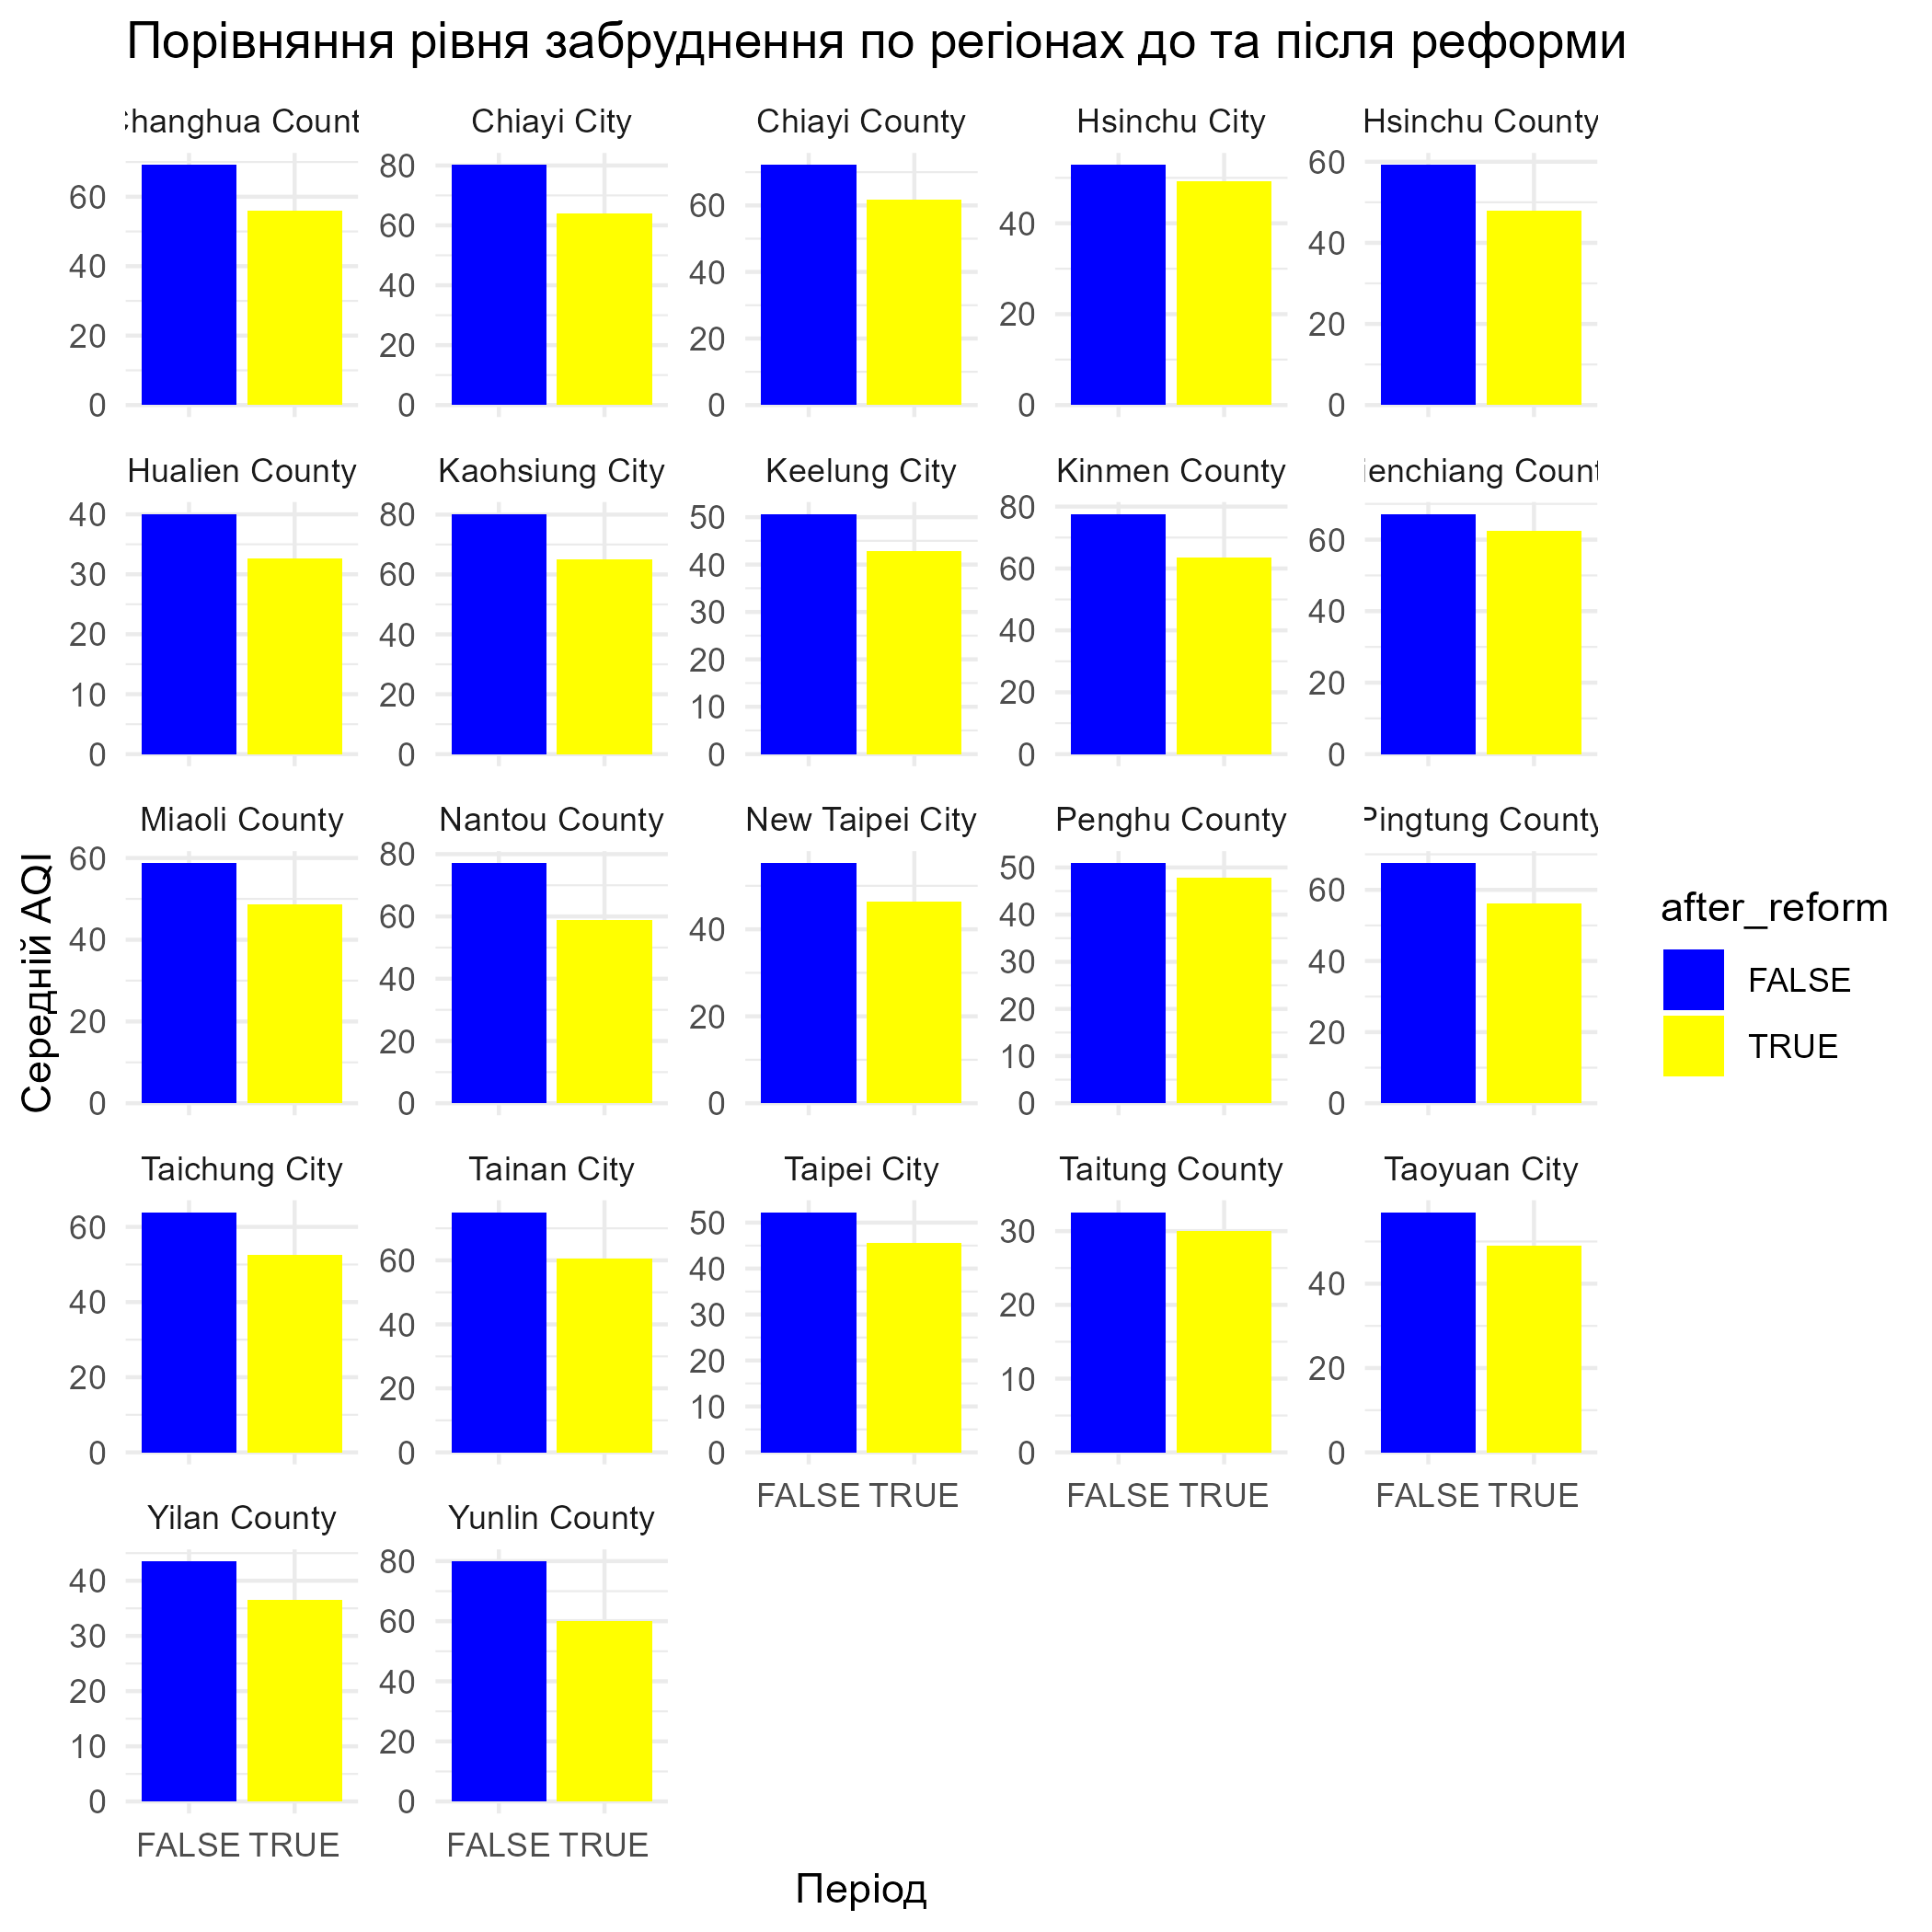
\includegraphics[width=\linewidth]{plots/question5/region_comparison_aqi.png}

  \pagebreak

  \item Чи існує залежність між початком реформ та показниками забруднення?

  \quad \textit{Був використаний tidy набір даних}

  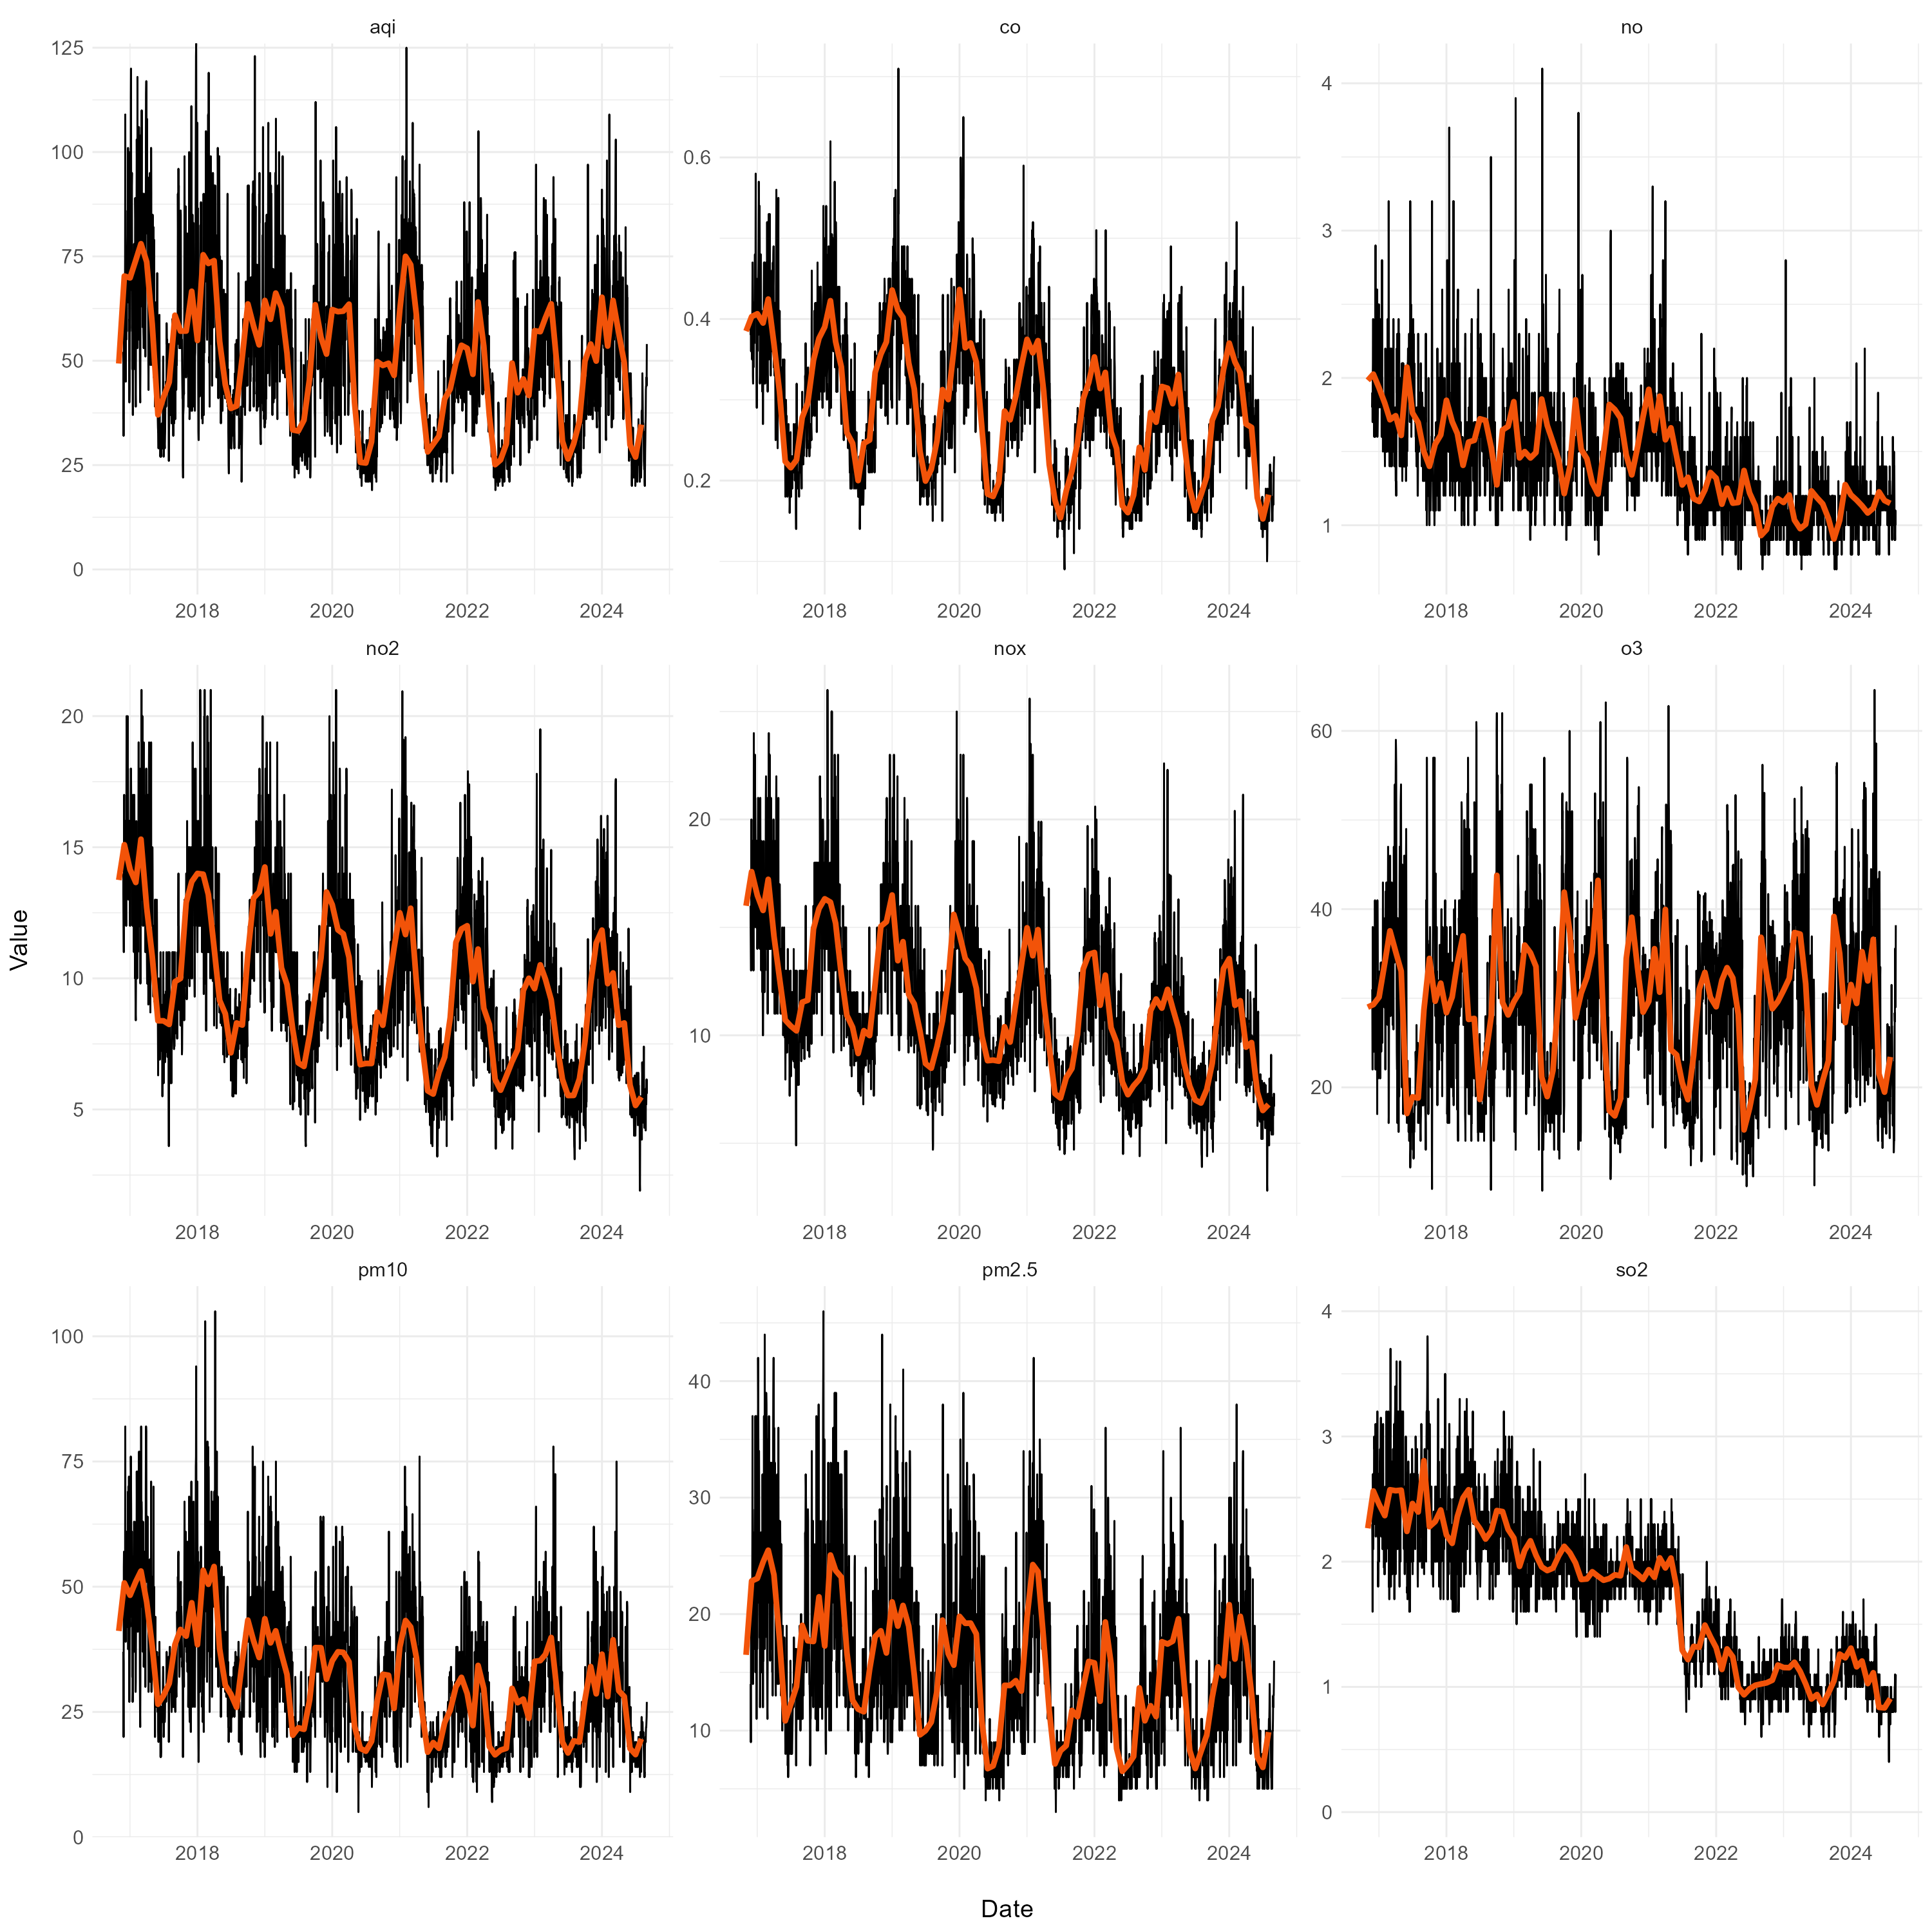
\includegraphics[width=\linewidth]{plots/question6/line.png}

  \pagebreak

  \item Як змінюється якість повітря залежно від станції виміру у містах?

  \quad \textit{Був використаний trimmed набір даних}

  Будемо розглядати зміни в показниках якості повітря в певній точці в часі (наприклад, 2023-06-28 11:00:00) в
  конкретному регіоні (наприклад, Tainan). Таким чином, будемо розглядати датасет
  згрупований за парою \verb|(date; county)|, так як тілкьи $sitename$ різний в групі:
  єдиним, що є різним у групі є.

  Порахуємо узагальнену статистику по кількості рядків в кожній групі:

  \begin{tabular}{cccccc}
    \textbf{Min.} & \textbf{1st Qu.}  & \textbf{Median} & \textbf{Mean} & \textbf {3rd Qu.} & \textbf{Max.} \\
    1 &  1  & 3 & 3.864 & 5 & 26 \\
  \end{tabular}

  Середня величина групи в кожному регіоні:

  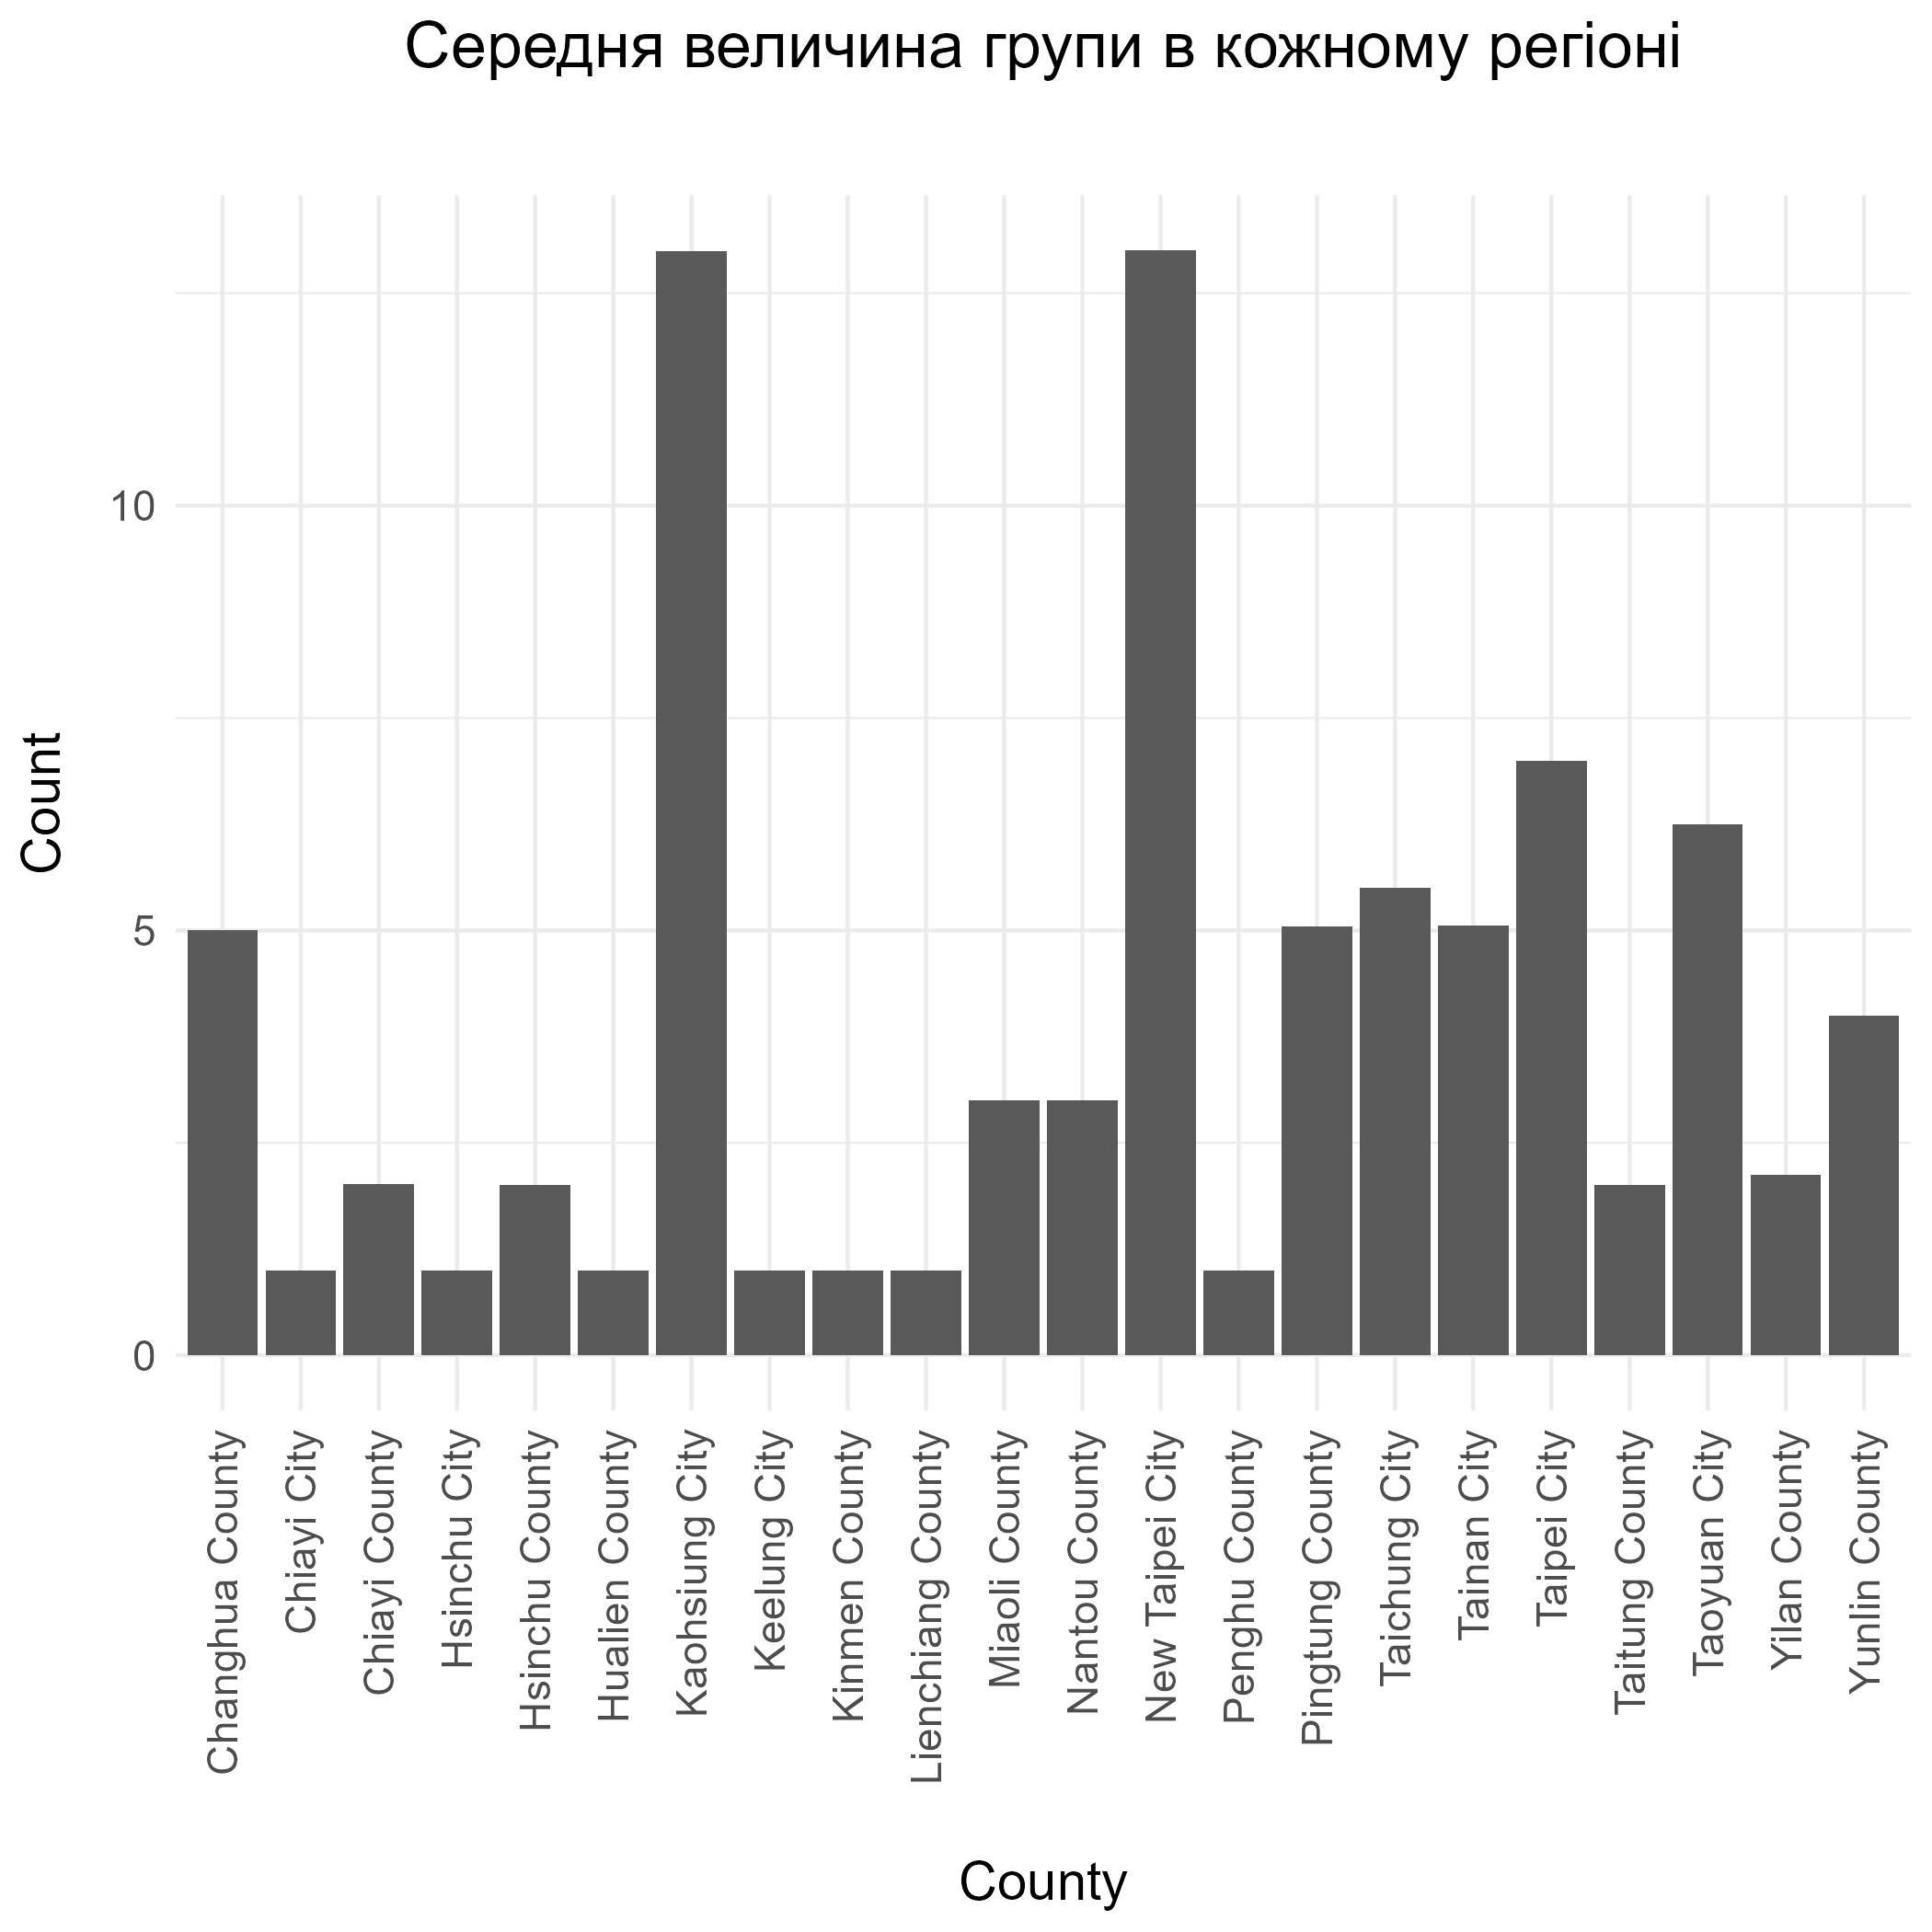
\includegraphics[width=\linewidth]{plots/question7/bar-count.png}

  Для аналізу змін в групі, будемо використовувати \textit{Median absolute difference}.

  \pagebreak

  Дескрептивні статистики:

  \begin{tabular}{lcccccc}
    \hline
    \textbf{Variable} & \textbf{Min.} & \textbf{1st Qu.}  & \textbf{Median} & \textbf{Mean} & \textbf{3rd Qu.} & \textbf{Max.} \\
    \hline
    \textbf{aqi}      & 0 & 0 & 2.965  & 4.597  & 6.672  & 109.712 \\
    \textbf{so2}      & 0 & 0 & 0.2224 & 0.2989 & 0.4448 & 58.8592 \\
    \textbf{co}       & 0 & 0 & 0.0222 & 0.0405 & 0.0593 & 4.0846  \\
    \textbf{o3}       & 0 & 0 & 2.076  & 3.268  & 5.041  & 56.191  \\
    \textbf{pm10}     & 0 & 0 & 2.965  & 4.265  & 5.930  & 254.266 \\
    \textbf{pm2.5}    & 0 & 0 & 1.483  & 2.424  & 3.707  & 137.141 \\
    \textbf{no2}      & 0 & 0 & 1.038  & 2.026  & 2.965  & 36.472  \\
    \textbf{nox}      & 0 & 0 & 1.26   & 2.57   & 3.558  & 71.61   \\
    \textbf{no}       & 0 & 0 & 0.2965 & 0.6151 & 0.593  & 62.2692 \\
  \end{tabular}

  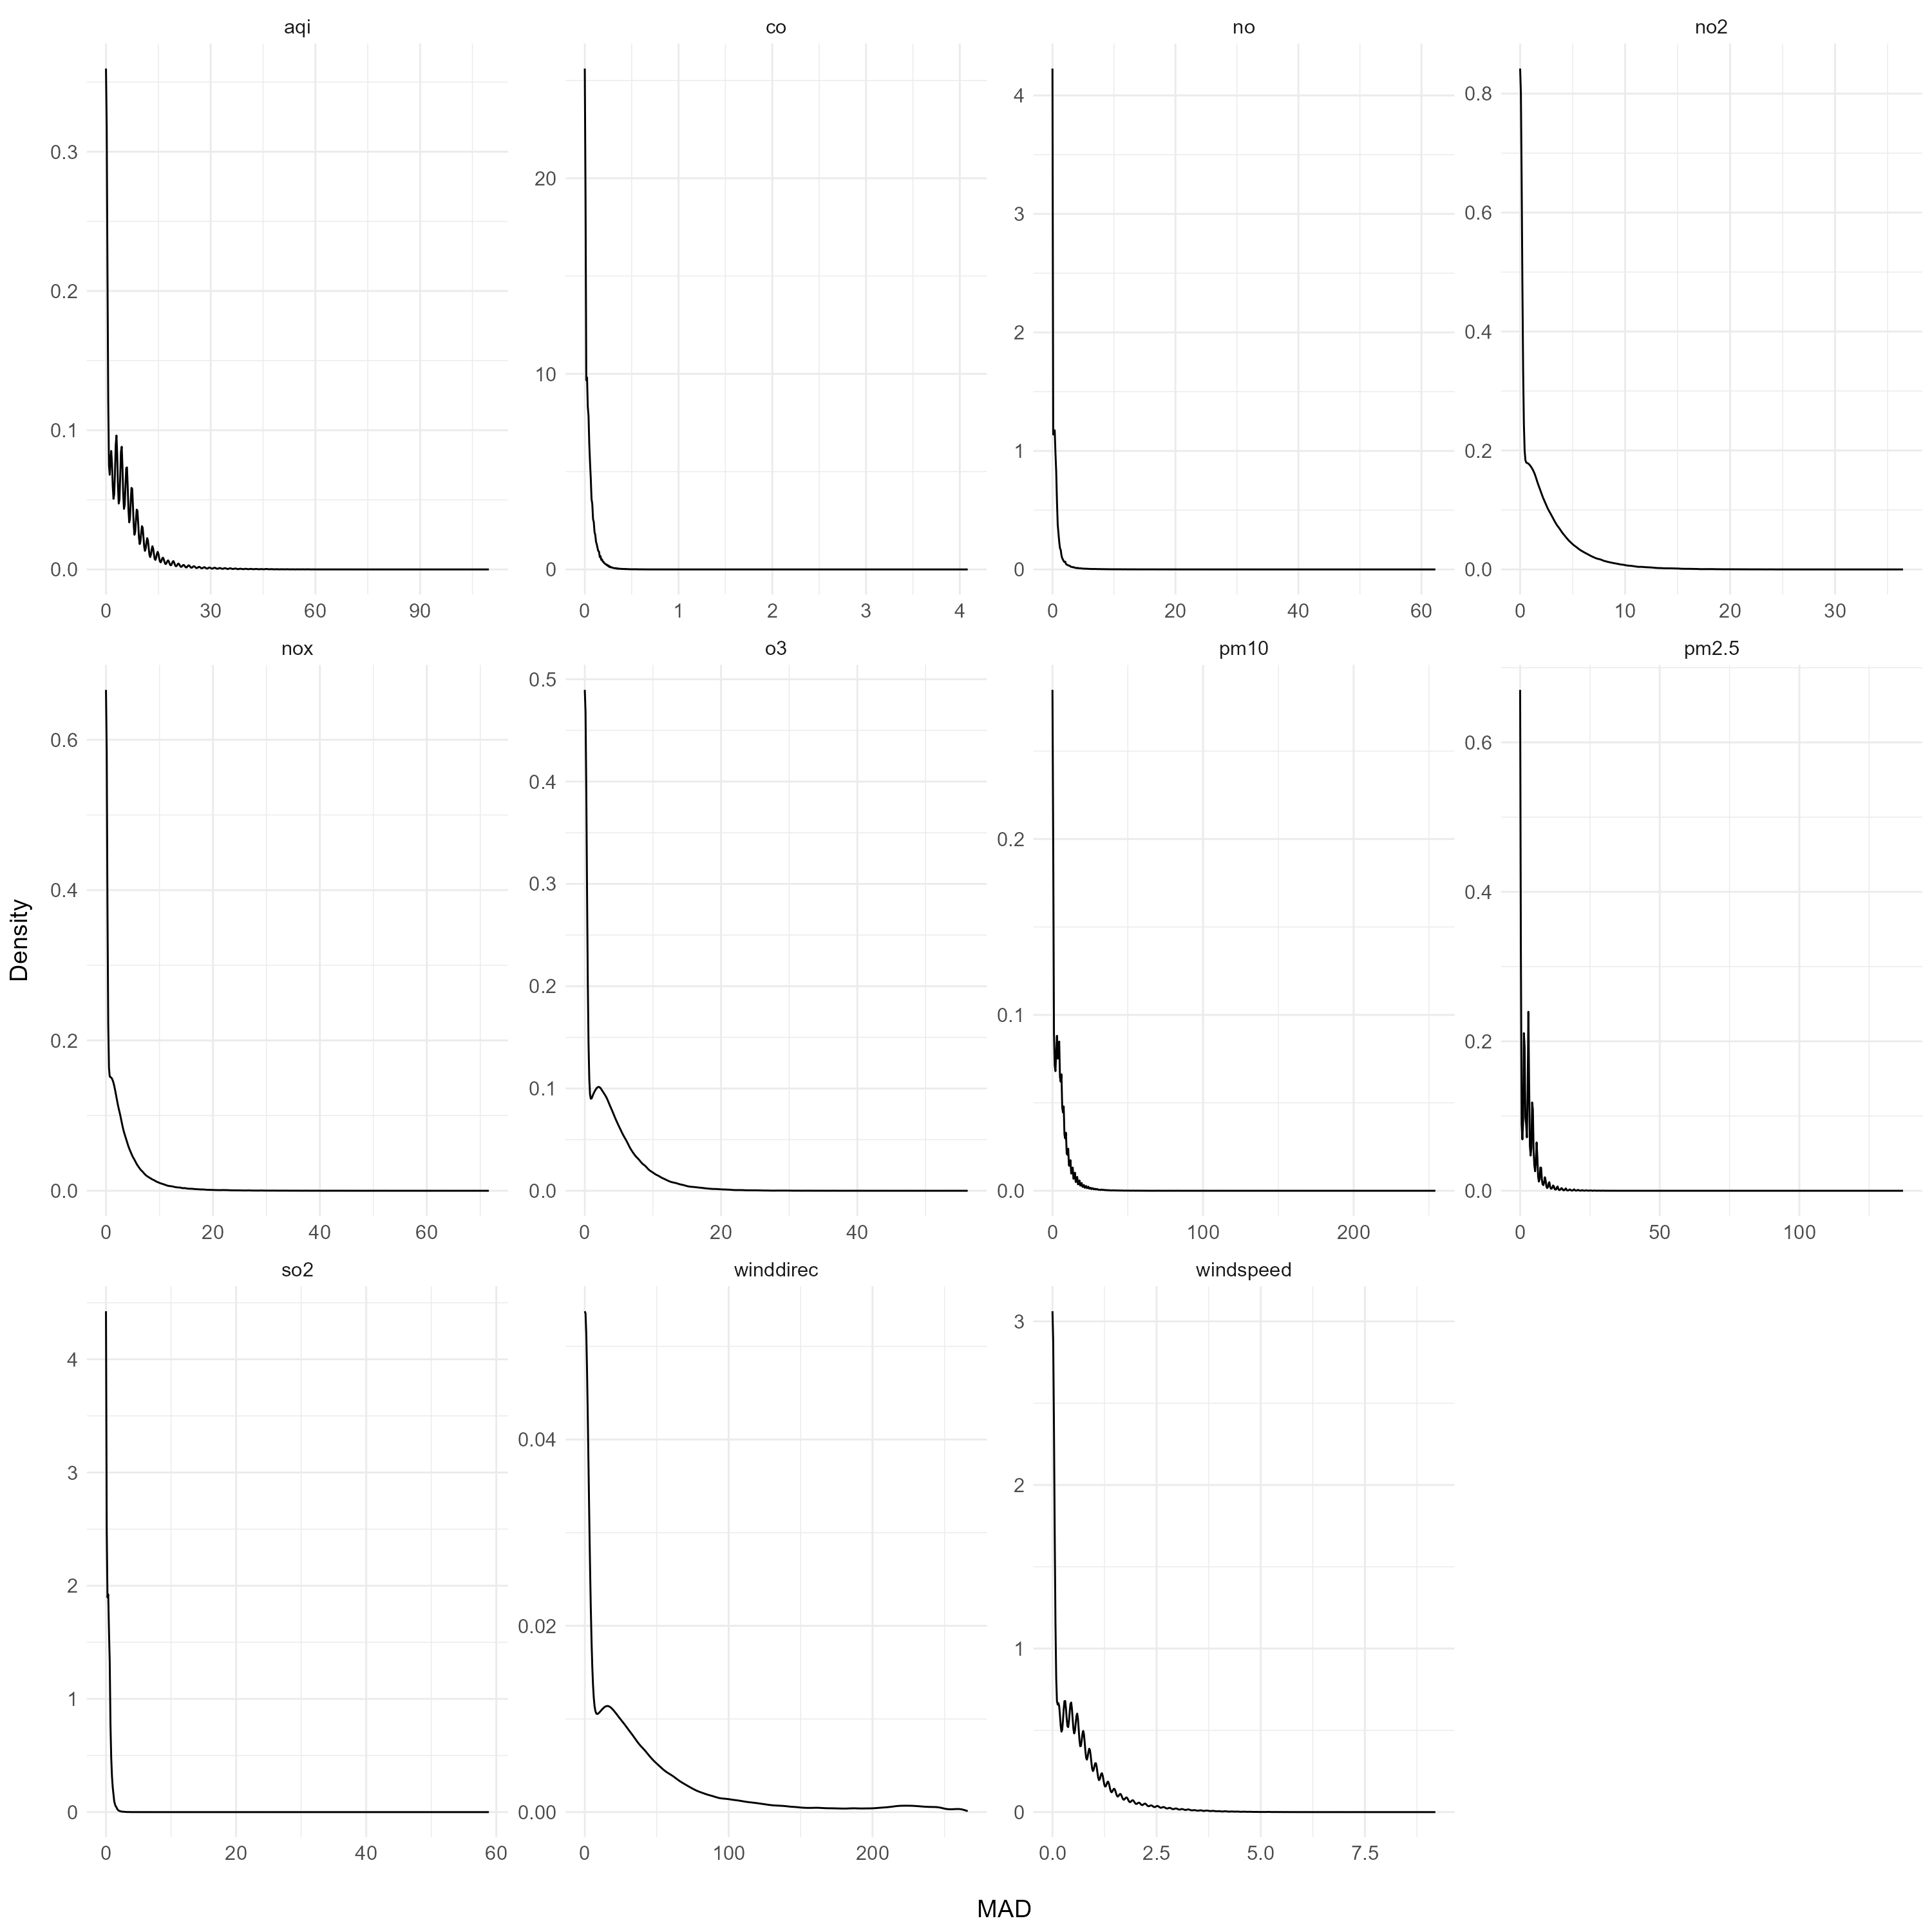
\includegraphics[width=\linewidth]{plots/question7/density.png}

  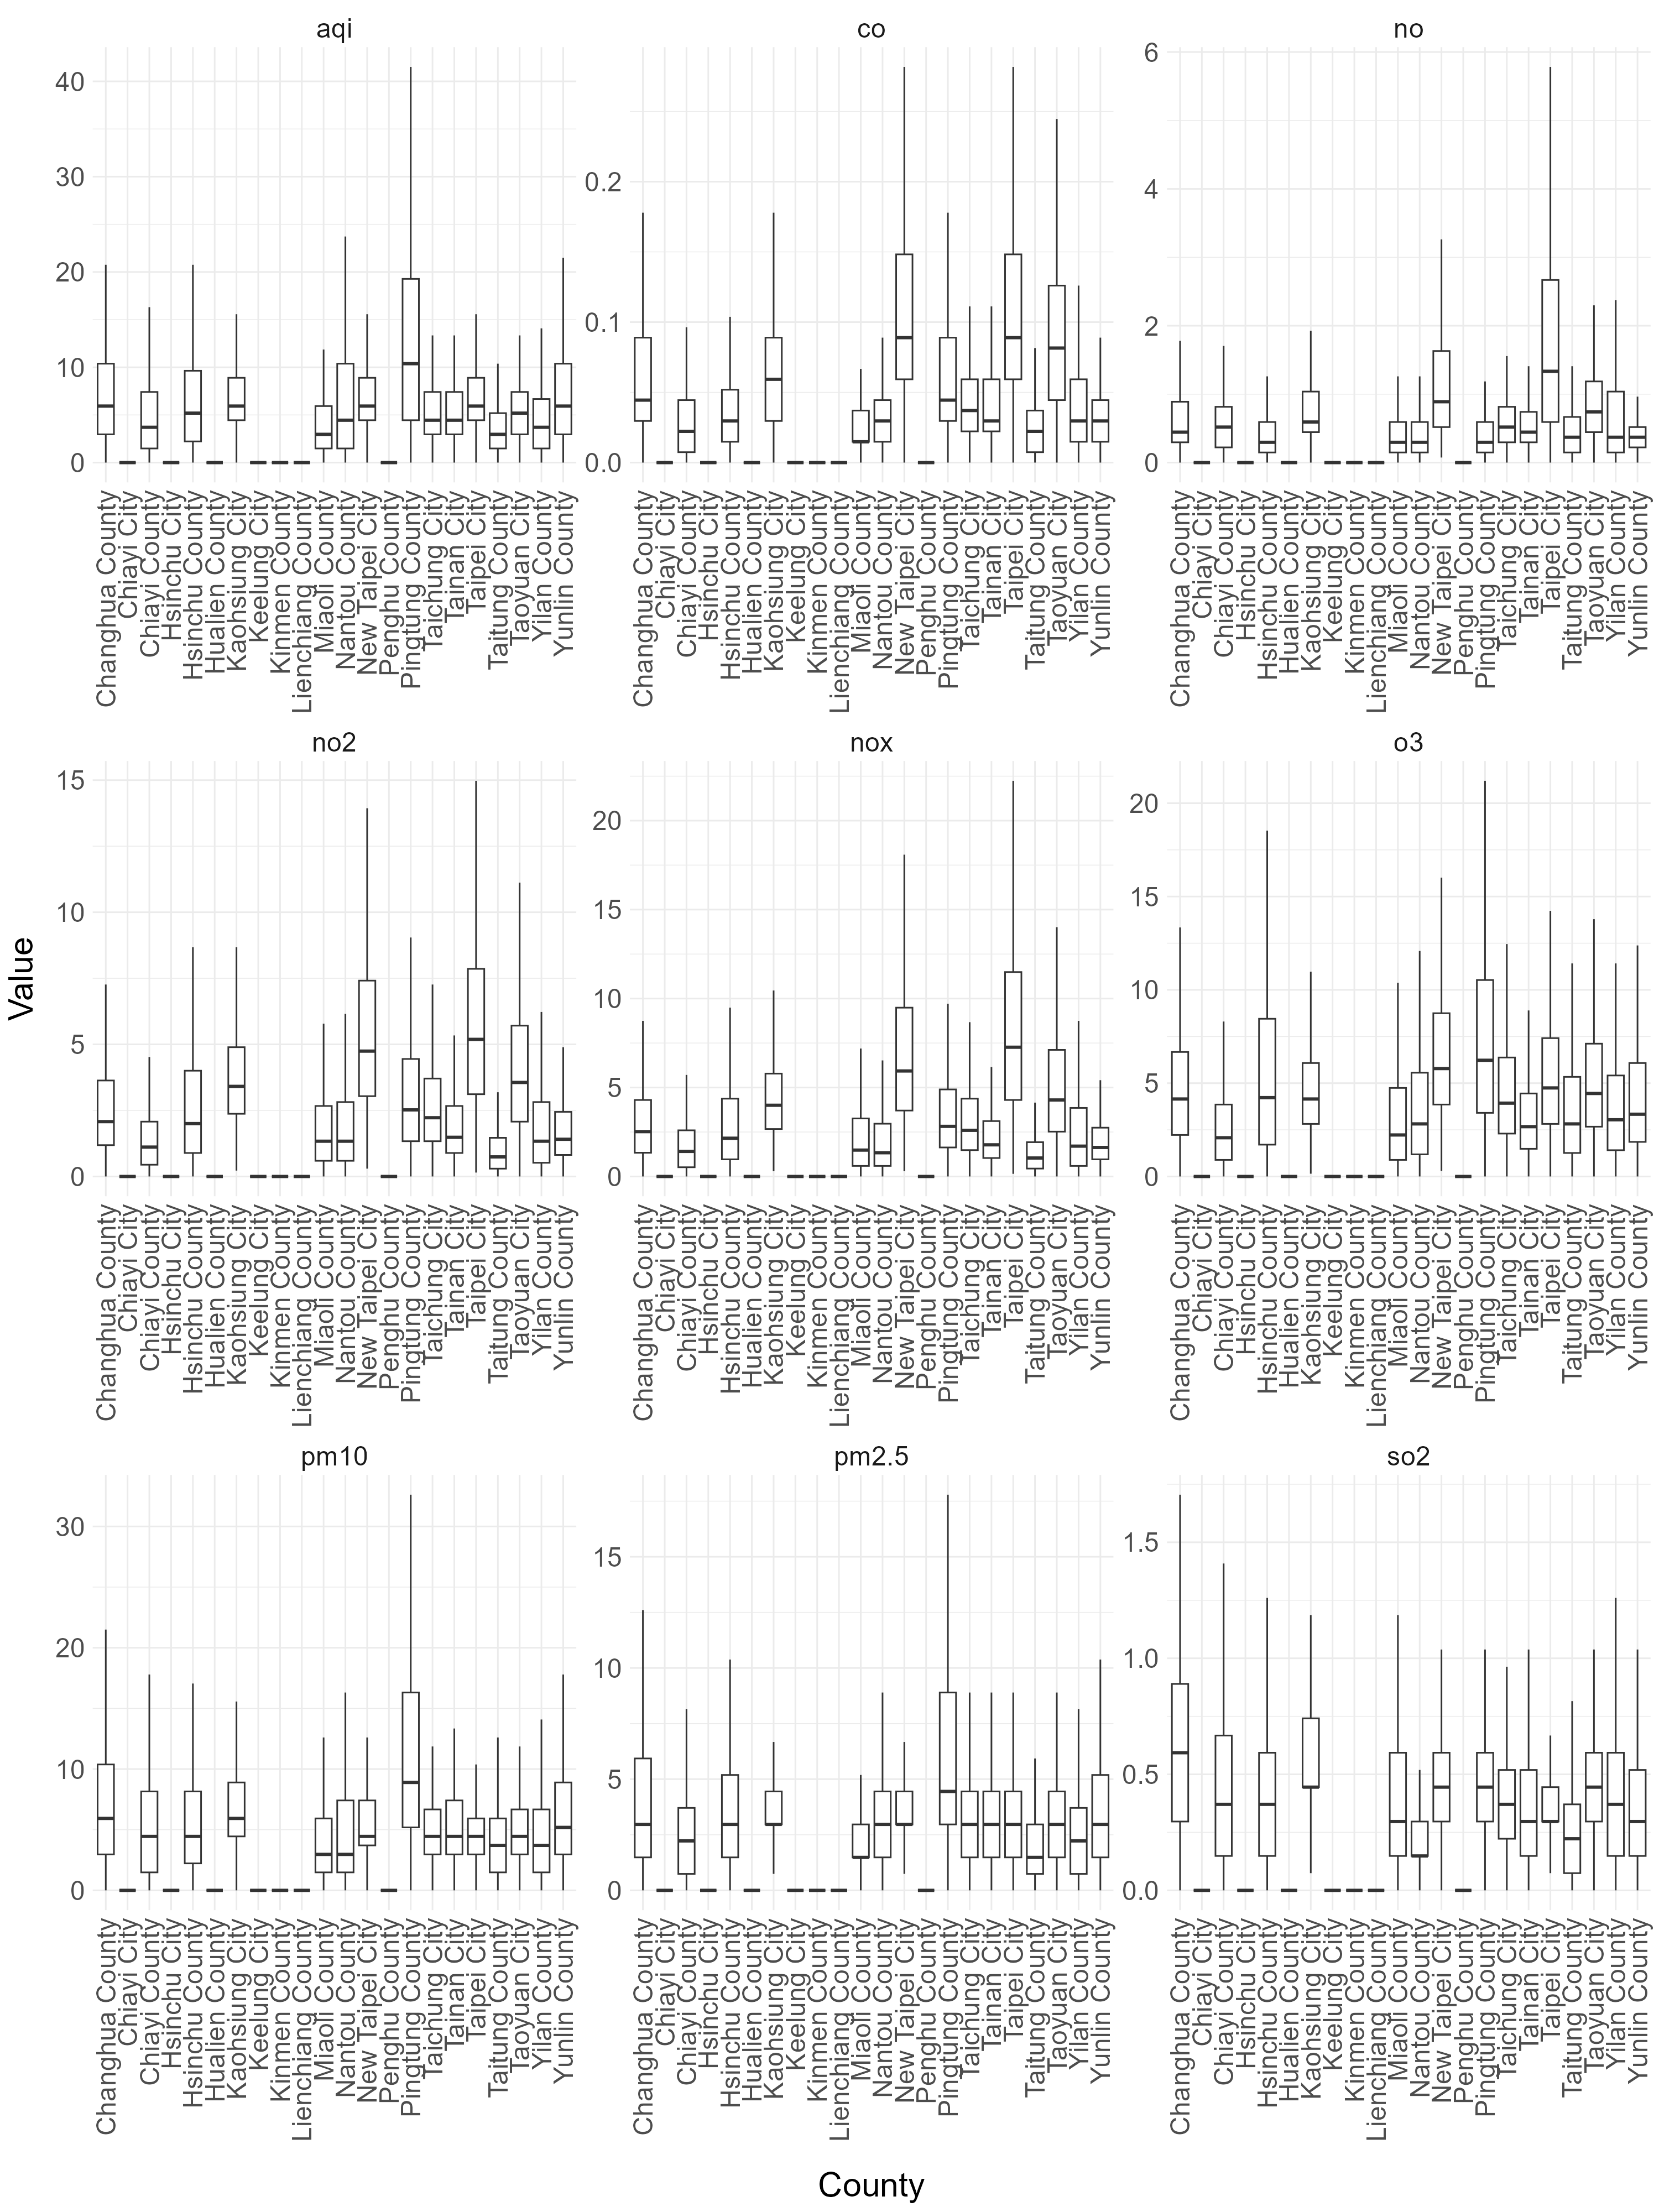
\includegraphics[width=\linewidth]{plots/question7/box-county.png}
\end{enumerate}

\end{document}